% \documentclass[conference]{IEEEtran}
% \IEEEoverridecommandlockouts
% % The preceding line is only needed to identify funding in the first footnote. If that is unneeded, please comment it out.
% \usepackage{cite}
% \usepackage{amsmath,amssymb,amsfonts}
% \usepackage{algorithmic}
% \usepackage{graphicx}
% \usepackage{textcomp}
% \usepackage{xtab}
% \usepackage{xcolor}
% \usepackage{caption}
% \usepackage[utf8]{inputenc}
% \usepackage{float} % [H] 옵션을 사용하기 위해 추가

% \usepackage{array}
% \usepackage{longtable} % 표가 길 경우 자동으로 다음 페이지로 넘기기 위해 사용
% \usepackage{geometry} % 페이지 여백 설정

% \geometry{a4paper, margin=1in}
% \pagestyle{plain}
% \pagenumbering{arabic}

% \def\BibTeX{{\rm B\kern-.05em{\sc i\kern-.025em b}\kern-.08em
%     T\kern-.1667em\lower.7ex\hbox{E}\kern-.125emX}}
    
% \begin{document}



% \documentclass[conference]{IEEEtran}
% \IEEEoverridecommandlockouts
% % 필요한 패키지 추가
% \usepackage{kotex} % 한글 지원
% \usepackage{longtable} % 긴 표를 여러 페이지에 걸쳐 표시
% \usepackage{geometry} % 여백 설정
% \usepackage{array} % 표 열 폭 설정
% \usepackage{caption} % 표 캡션 스타일링
% \geometry{a4paper, margin=1in}
% \usepackage{cite}
% \usepackage{amsmath,amssymb,amsfonts}
% \usepackage{algorithmic}
% \usepackage{graphicx}
% \usepackage{textcomp}
% \usepackage{xtab}
% \usepackage{xcolor}
% \usepackage{caption}
% \usepackage[utf8]{inputenc}
% \usepackage{float} % [H] 옵션을 사용하기 위해 추가

% \usepackage{array}
% \usepackage{longtable} % 표가 길 경우 자동으로 다음 페이지로 넘기기 위해 사용
% \usepackage{geometry} % 페이지 여백 설정

% \geometry{a4paper, margin=1in}
% \pagestyle{plain}
% \pagenumbering{arabic}

% \def\BibTeX{{\rm B\kern-.05em{\sc i\kern-.025em b}\kern-.08em
%     T\kern-.1667em\lower.7ex\hbox{E}\kern-.125emX}}
% \begin{document}

\documentclass[conference]{IEEEtran}
\IEEEoverridecommandlockouts

% 필요한 패키지 추가
\usepackage{kotex} % 한글 지원
\usepackage{longtable} % 긴 표를 여러 페이지에 걸쳐 표시
\usepackage{array} % 표 열 폭 설정
\usepackage{caption} % 표 캡션 스타일링
\usepackage{cite} % 참고문헌
\usepackage{amsmath,amssymb,amsfonts} % 수학 기호
\usepackage{algorithmic} % 알고리즘 환경
\usepackage{graphicx} % 그래픽 포함
\usepackage{textcomp} % 특수 문자
\usepackage{xcolor} % 색상 지원
\usepackage{float} % [H] 옵션을 사용하기 위해 추가

% 페이지 스타일 및 넘버링 설정
\pagestyle{plain}
\pagenumbering{arabic}

% BibTeX 정의
\def\BibTeX{{\rm B\kern-.05em{\sc i\kern-.025em b}\kern-.08em
    T\kern-.1667em\lower.7ex\hbox{E}\kern-.125emX}}
    
\begin{document}

\title{HeartLink \\
    {\textsuperscript{}-An AI Family Platform for Rebuilding Connection-}
    }

\author{\IEEEauthorblockN{1\textsuperscript{st} Jeong Yeonkyung}
\IEEEauthorblockA{\textit{Dept. of Information Systems } \\
\textit{Hanyang Univ.}\\
Seoul, Republic of Korea \\
edaily0129@gmail.com}
\and
\IEEEauthorblockN{2\textsuperscript{nd} Kim Dayeon}
\IEEEauthorblockA{\textit{Dept. of Information Systems } \\
\textit{Hanyang Univ.}\\
Seoul, Republic of Korea \\
jewelry0706@hanyang.ac.kr}
\and
\IEEEauthorblockN{3\textsuperscript{rd} Park Jeongho}
\IEEEauthorblockA{\textit{Dept. of Information Systems } \\
\textit{Hanyang Univ.}\\
Seoul, Republic of Korea \\
popramel@hanyang.ac.kr}
\and
\IEEEauthorblockN{4\textsuperscript{th} Yu Jihye}
\IEEEauthorblockA{\textit{Dept. of Information Systems } \\
\textit{Hanyang Univ.}\\
Seoul, Republic of Korea \\
jihyeyu33@hanyang.ac.kr}
}

\maketitle
\thispagestyle{plain}

\begin{abstract}
In today's fast-paced world, staying connected with family and loved ones can be challenging, particularly for intergenerational families facing digital barriers. This project introduces a voice-based social networking service that transcends the limitations of text and photos, fostering natural and seamless daily sharing. Leveraging advanced AI technologies such as Whisper fine-tuned for Korean speech recognition, DALLE-3 for image generation, and ChatGPT for natural conversations with characters , our platform allows users to share their lives through voice inputs that transform into text and image feeds. This approach enhances family connections without requiring manual content creation.\\

The application's key features include a shared group feed for real-time updates, voice-to-text conversion, and AI-generated images based on textual input, enabling users to capture daily moments authentically. There are additional functionalities like group album that collects memories and a virtual chatbot pet CLOi that makes SNS more fun to enjoy. With simple, voice-enabled interactions, users of all ages can effortlessly participate in family communication, making it a meaningful part of their daily routine.
\end{abstract}

\begin{IEEEkeywords}
Voice-based sharing, Family communication, AI-powered feed, Intergenerational connection, Auto speech recognition, Image generation, Memory preservation, Daily moments, Group photo album, Virtual pet CLOi
\end{IEEEkeywords}

\section{Role Assignment}
% \begin{table}[htbp]
% \begin{tabular}{|p{1cm}|p{1.7cm}|p{5cm}|}
%     \hline
%     Name & Roles & Task description and etc. \\
%     \hline
%     Jeong Yeonkyung &  Project Manager, Software Developer (Back-end) & Oversees the development team, ensuring that the project is completed on time and within budget. Plans and implements the development methodology, sets team goals and deliverables, and provides mentoring and guidance to developers. Ensures code quality and adherence to standards. As a back-end developer, manages server-side infrastructure, optimizes databases, and handles SQL queries to ensure smooth operation of web and mobile applications. Technologies used include Python, Node.js, and JavaScript.\\
%     \hline
%         \end{tabular}
% \end{table}
% \begin{table}[htbp]
%     \begin{tabular}{|p{1cm}|p{1.7cm}|p{5cm}|}
%     \hline
%     Kim Dayeon & Software Developer (Front-end), UI/UX Designer & As a front-end developer, leads the overall UI/UX page design of the software and personally carries out the development tasks. Ensures the user interface is not only visually appealing but also provides a seamless \\
%     \hline
%     \end{tabular}
% \end{table}

% \begin{table}[htbp]
% \begin{tabular}{|p{1cm}|p{1.7cm}|p{5cm}|}
%     \hline
%     & & and intuitive user experience. Uses design tools like Figma to meticulously refine visual elements and user interactions. Implements the design, ensuring a high level of interaction and functionality for users.\\
%     \hline
% \end{tabular}

%  \begin{tabular}{|p{1cm}|p{1.7cm}|p{5cm}|}
%     Park Jeongho & Developer Manager, Software Developer (Front-end) & As a front-end developer, designs and develops intuitive and efficient user interfaces based on user needs. Implements the interface using React-Native and JavaScript, ensuring easy navigation for users. Additionally, as a user/customer, contributes to making the service more accessible and usable for a wider audience.\\
%     \hline
%     Yu Jihye & Software Developer (AI), Product Planner& Responsible for product design and integrating AI features. Develops AI models based on user data, ensuring the system adapts to users' needs. Utilizes AI to provide personalized recommendations and automates repetitive tasks, enhancing the overall user experience.\\
%     \hline
% \end{tabular}
% \end{table}

\begin{table}[htbp]
\centering
\caption{Team Member Roles and Responsibilities}
\begin{tabular}{|p{1cm}|p{1.7cm}|p{5cm}|}
    \hline
    \textbf{Name} & \textbf{Roles} & \textbf{Task Description and etc.} \\
    \hline
    Jeong Yeonkyung & Project Manager, Software Developer (Back-end) & Oversees the development team, ensuring that the project is completed on time and within budget. Plans and implements the development methodology, sets team goals and deliverables, and provides mentoring and guidance to developers. Ensures code quality and adherence to standards. As a back-end developer, manages server-side infrastructure, optimizes databases, and handles SQL queries to ensure smooth operation of web and mobile applications. Technologies used include Python, Node.js, and JavaScript. \\
    \hline
    Kim Dayeon & Software Developer (Front-end), UI/UX Designer & As a front-end developer, leads the overall UI/UX page design of the software and personally carries out the development tasks. Ensures the user interface is not only visually appealing but also provides a seamless and intuitive user experience. Uses design tools like Figma to meticulously refine visual elements and user interactions. Implements the design, ensuring a high level of interaction and functionality for users. \\
    \hline
    Park Jeongho & Developer Manager, Software Developer (Front-end) & As a front-end developer, designs and develops intuitive and efficient user interfaces based on user needs. Implements the interface using React-Native and JavaScript, ensuring easy navigation for users. Additionally, as a user/customer, contributes to making the service more accessible and usable for a wider audience. \\
    \hline
    Yu Jihye & Software Developer (AI), Product Planner & Responsible for product design and integrating AI features. Develops AI models based on user data, ensuring the system adapts to users' needs. Utilizes AI to provide personalized recommendations and automates repetitive tasks, enhancing the overall user experience. \\
    \hline
\end{tabular}
\end{table}


\section{Introduction}
    \subsection{Motivation}
    Just Speak, and Stay Connected

    Communication remains essential to all relationships. However, as our lives grow increasingly busy, maintaining natural and effortless connections becomes ever more challenging. While we commonly share our daily lives through texts and photos, these methods can sometimes lose their authenticity. Now, there is a need for a new mode of connection—one that allows us to capture and share moments through voice.

    With advancements in voice recognition and AI technology, this vision has become achievable. Particularly in family communication, a system that records daily moments through voice and automatically generates a feed for sharing can profoundly enhance connections. By converting voice-recorded moments into text and images, and automatically delivering these to family members, this system allows for more seamless and genuine communication between parents and children, as well as across generations.

    For instance, parents can stay updated on their children's daily lives without needing direct contact, while children can remain connected with family members through shared voice and visual updates. This voice-based interface not only bridges the digital divide between generations but also fosters a more natural and continuous flow of family communication.

    \subsection{Problem Statements}
        \subsubsection{Difficulty in Naturally Sharing Daily Life}
        Current social media platforms primarily rely on text input and photo uploads, making it challenging for users to capture and share their daily lives naturally. In situations where hands are occupied or real-time sharing is desired, users often have to interrupt or modify their experiences to create content that fits platform requirements. This compromises the authenticity of moments shared and makes it difficult to convey emotional depth in these interactions.
        
        \subsubsection{Generational Gaps in Digital Accessibility}
        Existing social media interfaces do not adequately address the accessibility differences that arise from variations in age and digital proficiency, which poses limitations for intergenerational family communication. Elderly users often find complex text input methods and intricate menu structures challenging, while younger children may struggle to express themselves naturally within traditional interfaces. These generational gaps hinder regular family communication, creating the risk that the perspectives and experiences of certain family members may be excluded from the family's shared narrative.
        
        \subsubsection{Limitations of Personalized Communication}

 Existing social media platforms (e.g., Instagram, Facebook) have a structure where feeds are public to all followers, which limits personalized communication. It is difficult for users to selectively restrict the content they want to share based on different relationships and situations, such as with family, friends, or coworkers. As a result, users often upload content that can be shared with everyone, rather than natural, personal moments. This structure makes it hard to authentically share personal emotions and experiences, which can ultimately lead to communication on social media becoming monotonous and formal.


    \subsection{Solution}
        \subsubsection{Voice-Based Daily Sharing}
        Voice input alone enables natural daily sharing. When speaking about daily experiences or thoughts, these vocal expressions automatically transform into text with relevant generated images, creating complete feeds. This direct voice-to-feed conversion eliminates manual text input or photo selection, making daily sharing effortless, especially during busy routines.

        \subsubsection{Cross-Generational Connection through Intuitive Interface and Automatic Generation}
        Automatic content creation and a user-friendly interface remove digital barriers with simple conversation, without the need for complicated processes. The system automatically converts spoken words into text and generates relevant content, making it easy for elderly family members who may not be familiar with digital technology to communicate. Children can also express themselves freely through natural speech, with content automatically generated to match their expressions. This approach bridges generational technology gaps and creates an inclusive environment where every family member can naturally participate in daily sharing.

        \subsubsection{Group Feed Service for Sharing with Selected Groups}
        Users can create desired groups (such as family, friends, coworkers, etc.) and share their feeds only with specific groups. This feature allows communication tailored to different relationships and situations. For example, users can share personal moments with family while sharing work-related updates with colleagues, ensuring that content is appropriate for each group. This group feed service enhances the user experience by enabling more personal and natural communication, helping to maintain more meaningful relationships on social media.

    \subsection{Research on Any Relative Software}
        \subsubsection{OpenAI DALL-E 3}
        Transforms daily moments into natural visual expressions. Creates high-quality images within two seconds based on voice or text input, adjusting styles to reflect conversational context and emotions. Generates safe, family-friendly images that richly express family moments and feelings while maintaining creative authenticity.

\section{Requirement Analysis}
    \subsection{Common Features}
        \subsubsection{Sign-Up}
            Users can sign up to access all AI features such as voice-based daily sharing, AI-generated images, family/friend photo album, virtual pet "CLOi", and cloud storage management. After signing up, access to additional features, such as personal data management and device linking, is determined based on user permissions.
            \begin{itemize}
                % \item Enter phone number : The phone number is verified through an authentication system.
                \item Enter email : The email is used for login purposes
                \item Enter password : Passwords must be at least 6 characters long
                \item Enter name : The name is used as the user's default nickname on the platform.
            \end{itemize}

        \subsubsection{Log in}
            Users can access all AI features such as voice-based daily sharing, AI-generated images, family/friend photo album, virtual pet "CLOi", and cloud storage management through a single log-in. After logging in, access to administrative functions like personal data and linked device management is determined by user permissions.

        % \subsubsection{Find ID/Password}
        %     Users can retrieve their ID via email or phone number. If they forget their password, the platform provides a reset option through authentication via registered phone numbers or emails.

    \subsection{User-Specific Features}
        \subsubsection{Main Feed}
            The group feed is a space where users can see posts from themselves, family members, and friends. Through this feed, users can check real-time updates and share their daily moments effortlessly. Our app leverages AI functionality to help users easily create posts to share their lives. On the main screen, users can select a specific group, allowing posts to be visible only to that selected group.

            When creating a post, users can either compose it manually or choose from three AI-based post creation features:
            \begin{itemize}
                \item Text-Based Image Generation: Based on the text written by the user or text created by AI based on users' voice input, AI generates an image. This allows users to include appropriate images in their posts without directly uploading photos, by generating images that match the written content.
            \end{itemize}

        \subsubsection{Post Archive}
            % By tapping the 'Archive' button in the bottom navigation bar, users can access a personal archive where only their own posts are stored. Here, users can easily manage their posts, adjusting visibility settings (public/private), as well as editing or deleting specific posts.
            This archive is a space where users can systematically store and manage their personal and group posts. Posts are organized chronologically, making it easy to find previous posts. Users can adjust visibility settings (public/private) or edit and delete specific posts. The archive securely stores important moments, serving as more than just a storage space—it’s a valuable tool for reminiscing about meaningful moments.

        \subsubsection{Family/Friends Shared Photo Album}
            % Users can create albums (folders) and select specific photos from their feed to include in these albums. By organizing photos into albums, users can manage which photos are displayed, and they can designate access permissions for each album, allowing only family members or close friends to view them.
            The group album feature allows group members to organize shared memories through photos. Users can view not only the photos they have posted on the feed but also those uploaded by other group members, all in one place within the group album. By creating albums (folders), users can organize photos and set access permissions for each album, ensuring that only specific group members (e.g., family, friends) can view them.The group album goes beyond merely organizing photos—it helps relive shared moments vividly and meaningfully.

        \subsubsection{Adding Friends}
            Although this SNS primarily focuses on family interaction, users can also add friends to share photos with them. This feature is designed for users who want to communicate with friends as well as family members.

        \subsubsection{Raising Our Family's Pet CLOi}
            % To motivate family participation in the SNS, we introduced a feature to raise a virtual pet called "CLOi." Similar to the "Sumone" app, this pet character grows based on the frequency of posts and photo uploads. It encourages group members to participate actively and promotes family bonding.
            To encourage family participation in the SNS, we introduced a virtual pet feature called "CLOi." This virtual pet interacts with users and plays a key role in fostering engagement. Through CLOi, users can build emotional connections and have natural conversations, enhancing the overall experience. CLOi's growth stages change based on user activity, motivating consistent participation in the app. Additionally, users can interact with CLOi through a chatbot feature.

\section{Development Environment}
    \subsection{Choice of Software Development Platform}
        \subsubsection{Estimated Cost}
            \begin{itemize}
                \item AWS EC2 \& S3: About 3 USD per month
                \item Google Colab Pro: 9.99 USD per month
            \end{itemize}
        
        \subsubsection{Development Platform}
            \begin{description}
                \item{Windows:}
                    Windows serves as our primary development platform, providing comprehensive support for React Native and Node.js development environments. It offers seamless integration with essential development tools and frameworks, enhancing overall development productivity. Windows' user-friendly interface simplifies environment configuration and project management, while its robust community support ensures quick problem resolution. The platform's continuous updates and improvements guarantee access to the latest development technologies, making it an ideal choice for our cross-platform mobile application development.
            \end{description}

        \subsubsection{Programming Languages} 
            \begin{description}
                \item{JavaScript:}
                    JavaScript stands as our core programming language, offering versatility for both frontend and backend development. Its extensive ecosystem and wide community support provide numerous libraries and tools essential for modern web development. JavaScript's interpreted nature enables rapid development and easy debugging, while its asynchronous capabilities make it particularly suitable for building responsive applications. The language's ubiquity ensures excellent documentation and resource availability, significantly enhancing development efficiency.
                \item{Python:}
                    Python is a programming language highly suited for AI development, especially in the fields of machine learning and data analysis. Its concise and intuitive syntax enables fast and efficient development, and various libraries and frameworks (e.g., TensorFlow, PyTorch, Scikit-learn) are extremely helpful in implementing complex AI algorithms. Additionally, Python provides powerful tools for data processing and analysis, making it suitable not only for AI model development but also for data preparation and preprocessing. As a result, Python plays a crucial role in AI and machine learning projects.
            \end{description}

        \subsubsection{Frameworks \& Database}
            \begin{itemize}
                \item React Native: React Native emerges as our primary framework for mobile application development. This JavaScript-based framework enables the development of native mobile applications for both iOS and Android platforms. React Native's component-based architecture promotes code reusability and maintainable structure, while its hot reloading feature accelerates the development process by enabling immediate code change verification. The framework's bridge to native components ensures high performance and authentic native user experiences, making it an optimal choice for our mobile application development.

                \item Express.js: Express.js functions as our backend framework, providing a minimalist yet robust solution for building web applications and APIs. Built on Node.js, it offers excellent performance for handling asynchronous operations and real-time data processing. The framework's middleware system allows for flexible request handling and modular application structure. Express.js's seamless integration with MongoDB through Mongoose enables efficient database operations, while its extensive ecosystem of middleware packages enhances development capabilities.

                \item MongoDB: MongoDB serves as our primary database system, offering a flexible and scalable NoSQL solution for our application's data management needs. Through Mongoose ODM (Object Data Modeling), it provides a structured way to model application data and enforce data schemas while maintaining MongoDB's dynamic nature. MongoDB's document-oriented structure aligns perfectly with JavaScript's JSON format, making it naturally compatible with our Node.js/Express.js backend. The database's powerful querying capabilities, along with its ability to handle large volumes of unstructured data, make it ideal for social media applications that require efficient storage and retrieval of various content types including user profiles, posts, and media metadata. Its scalability and performance in handling concurrent operations make it particularly suitable for real-time applications with frequent data updates and complex data relationships. 

                \item HuggingFace: HuggingFace Transformers provides our core framework for natural language processing tasks, specifically for fine-tuning the Whisper model for Korean speech recognition. The framework offers pre-trained models, optimization tools, and comprehensive APIs that streamline the model development process. We leveraged HuggingFace's dataset repository to access pre-processed Zeroth-Korean data for training. Additionally, HuggingFace Hub serves as our model storage and deployment platform, enabling seamless model versioning and API-based inference in production environments.

                \item FastAPI: FastAPI serves as our backend web framework, providing high-performance RESTful API endpoints for AI model integration. Its asynchronous capabilities and automatic OpenAPI documentation facilitate efficient handling of concurrent requests and seamless integration with our AI models. The framework's Python-based architecture ensures type safety and enables straightforward implementation of API endpoints for model inference.
            \end{itemize}

            \subsection{Software in Use}
        \begin{figure}[htbp]
            \centerline{
\includegraphics[width=3cm, height=3cm]{Images/logo/vsc.png}}
            \caption{Logo of Visual Studio Code}
            \label{fig}
        \end{figure}
        \subsubsection{Visual Studio Code (VS Code)}
            Visual Studio Code, commonly known as VS Code, is a lightweight yet powerful code editor developed by Microsoft. It supports various programming languages and provides essential tools like syntax highlighting, debugging, and integrated Git support. VS Code is highly extensible, allowing developers to customize the editor through a vast library of extensions to suit their specific needs. The editor's user-friendly interface and frequent updates contribute to its popularity among developers. Its ability to handle large codebases and quick access to useful extensions make it ideal for both web and mobile development.

        \begin{figure}[htbp]
            \centerline{
\includegraphics[width=3cm, height=3cm]{Images/logo/android.png}}
            \caption{Logo of Android Studio}
            \label{fig}
        \end{figure}
        \subsubsection{Android Studio}
            Android Studio serves as the primary integrated development environment (IDE) for Android application development. It provides comprehensive tools essential for React Native development, including the Android SDK manager, device emulators, and debugging capabilities. The platform's advanced emulator system allows developers to test applications across various Android versions and device configurations, ensuring broad compatibility. Android Studio's performance profiling tools help optimize application performance, while its integrated debugging features enable efficient problem resolution. With built-in support for version control systems and continuous integration, Android Studio streamlines the development workflow for mobile applications.

        \begin{figure}[htbp]
            \centerline{
\includegraphics[width=3cm, height=3cm]{Images/logo/expo.png}}
            \caption{Logo of Expo}
            \label{fig}
        \end{figure}
        \subsubsection{Expo}
            Expo is a framework and a platform for universal React applications, enabling developers to build, deploy, and maintain React Native applications more easily. It provides a set of tools and services, including a development client, pre-built libraries, and an online publishing platform, that streamline the app development process. With Expo, developers can preview changes instantly on physical devices without complex configurations. Expo also supports the integration of native modules, making it easier to access device-specific features. Its simplicity and support for hot reloading make Expo a popular choice for building cross-platform mobile apps.

        \begin{figure}[htbp]
            \centerline{
\includegraphics[width=4cm, height=3cm]{Images/logo/zustand.png}}
            \caption{Logo of Zustand}
            \label{fig}
        \end{figure}
        \subsubsection{Zustand}
            Zustand is a lightweight state management library for React applications. It provides a simple API for managing global state, allowing developers to avoid prop drilling by sharing state across components directly. Zustand's minimal setup and component-based approach make it easy to use and integrate into existing projects. The library supports both synchronous and asynchronous state updates, giving developers flexibility in handling complex state logic. Its simplicity and efficiency make Zustand an ideal choice for managing application state in a straightforward and maintainable way.

        \begin{figure}[htbp]
            \centerline{
\includegraphics[width=5cm, height=2cm]{Images/logo/figma.png}}
            \caption{Logo of Figma}
            \label{fig}
        \end{figure}
        \subsubsection{Figma}
            Figma is a collaborative design tool widely used for creating user interfaces, prototypes, and interactive design elements. Its web-based nature allows teams to work together in real-time, making it ideal for cross-functional collaboration between designers and developers. Figma supports a variety of design elements and offers tools for creating responsive designs, making it a versatile choice for UI/UX design. Developers can easily inspect design specs, export assets, and view design changes live, enhancing communication and workflow efficiency. With its user-friendly interface and cloud-based functionality, Figma has become a popular choice for modern design teams.

        \begin{figure}[htbp]
            \centerline{
\includegraphics[width=4cm, height=4cm]{Images/logo/aws.png}}
            \caption{Logo of Amazon EC2}
            \label{fig}
        \end{figure}
        \subsubsection{Amazon EC2}
            Amazon EC2 (Elastic Compute Cloud) is a part of Amazon Web Services (AWS) that provides scalable virtual servers in the cloud. Developers can configure and launch EC2 instances to run various applications, giving them control over the underlying computing resources. EC2 supports a wide range of instance types optimized for different workloads, including CPU-intensive and memory-intensive tasks. It is ideal for deploying web applications, backend services, and data processing workloads, as it allows for flexible scaling to meet demand. With robust security options and integration with other AWS services, EC2 is widely used in cloud-based infrastructures.

        \begin{figure}[htbp]
            \centerline{
\includegraphics[width=4cm, height=3cm]{Images/logo/awss3.png}}
            \caption{Logo of Amazon S3}
            \label{fig}
        \end{figure}
        \subsubsection{Amazon S3}
            Amazon S3 (Simple Storage Service) is a highly scalable cloud storage service provided by AWS, designed to store and retrieve any amount of data. It allows developers to create and manage buckets for organizing data, which can be used for hosting static websites, archiving, and data backups. S3's durability and high availability make it suitable for critical data storage, while its integration with other AWS services enhances data management flexibility. S3 also supports versioning and access controls, allowing for secure data storage and retrieval. This service is essential for applications requiring reliable and scalable storage solutions.

        \begin{figure}[htbp]
            \centerline{
\includegraphics[width=4cm, height=2cm]{Images/logo/google colab pro.png}}
            \caption{Logo of Google Colab Pro}
            \label{fig}
        \end{figure}
        \subsubsection{Google Colab Pro}
            Google Colab Pro served as our primary cloud-based development environment for AI model training and experimentation. It provides GPU acceleration support, significant computational resources, and seamless integration with essential machine learning libraries. The platform's interactive Jupyter notebook interface enabled efficient code development and model iteration. With its expanded memory allocation and longer runtime limits compared to the standard version, Colab Pro facilitated the training of complex deep learning models without requiring local high-performance hardware.

        \begin{figure}[htbp]
            \centerline{
\includegraphics[width=6cm, height=2cm]{Images/logo/postman.png}}
            \caption{Logo of Postman}
            \label{fig}
        \end{figure}
        \subsubsection{Postman}
            Postman functions as our API development and testing platform, enabling comprehensive testing and documentation of our REST APIs. It provides a user-friendly interface for creating, organizing, and executing HTTP requests, making API testing and debugging more efficient. The tool's ability to create test suites, set up automated testing environments, and generate API documentation streamlines the API development process. Postman's collaboration features allow team members to share collections and environments, ensuring consistency in API testing across the development team. Its request history and response validation features make it invaluable for API debugging and optimization.

        \begin{figure}[htbp]
            \centerline{
\includegraphics[width=6cm, height=2.5cm]{Images/logo/github.png}}
            \caption{Logo of GitHub}
            \label{fig}
        \end{figure}
        \subsubsection{GitHub}
            GitHub is an essential platform for version control and collaboration in software development. It provides a centralized repository for code, allowing multiple developers to work on the same project simultaneously and manage changes efficiently. Through features like pull requests, issue tracking, and branching, GitHub enables teams to review code, track project progress, and manage tasks effectively. It also integrates with numerous development tools, facilitating seamless workflows. With an active community and extensive documentation, GitHub supports both open-source and private projects, making it a versatile tool for developers.

        \begin{figure}[htbp]
            \centerline{
\includegraphics[width=4.5cm, height=3cm]{Images/logo/jira.png}}
            \caption{Logo of Jira}
            \label{fig}
        \end{figure}
        \subsubsection{Jira}
Jira is a powerful project management tool widely used for tracking tasks, issues, and project milestones, particularly in agile software development. It provides a robust framework for planning, monitoring, and managing workflows through features like customizable boards, sprint planning, and backlog prioritization. Its issue tracking system allows teams to create, assign, and resolve tasks efficiently, while integration with development tools ensures seamless collaboration across teams. Jira's advanced reporting and analytics, including burndown charts and velocity reports, enable better decision-making and project forecasting. With extensive customization options and support for plugins, Jira adapts to a wide range of industries and project needs, making it an indispensable tool for effective project management.


        \begin{figure}[htbp]
            \centerline{
\includegraphics[width=5.5cm, height=2cm]{Images/logo/notion.png}}
            \caption{Logo of Notion}
            \label{fig}
        \end{figure}
        \subsubsection{Notion}
            Notion is an all-in-one workspace that combines note-taking, project management, and knowledge sharing in one platform. Its flexible, block-based structure allows users to organize content in various formats, including text, tables, images, and databases, making it suitable for diverse tasks. Notion supports real-time collaboration, enabling team members to work on shared documents and tasks seamlessly. It is commonly used for creating wikis, project boards, and personal notes, as it provides extensive customization options. With its intuitive interface and robust features, Notion is a valuable tool for organizing and managing project information.


        \begin{figure}[htbp]
            \centerline{
\includegraphics[width=5cm, height=2cm]{Images/logo/overleaf.png}}
            \caption{Logo of Overleaf}
            \label{fig}
        \end{figure}
        \subsubsection{Overleaf}
            Overleaf is an online collaborative platform specifically designed for LaTeX document creation, popular among researchers, students, and academics. It provides a real-time LaTeX editor, allowing users to collaborate on complex documents containing mathematical equations, tables, and references. Overleaf simplifies the writing process by offering a LaTeX compiler with instant previews, enabling authors to see how their documents look as they type. The platform also supports version control and can integrate with GitHub, making it easy to manage large projects with multiple contributors. Overleaf’s cloud-based nature makes it accessible from any device, enhancing the document creation process for scientific writing.

    \section{Specification}
   \subsection{Loading Page}
        \begin{figure}[htbp]
            \centerline{
\includegraphics[width=3cm]{Images/page/loading.png}}
            \caption{Loading Page}
            \label{fig}
        \end{figure}
        % When an application communicates with servers, a delay is inevitable in the process. During the delay, it might show just a blank screen to users. To prevent users from getting a blank page, a loading screen will appear instead. This applies to all functions that require server communication.

        % This loading page UI is made by 'skeleton' from React Native. While receiving data from the server, components without received data shows that it is loading. In other words, while server is processing and receiving data after a http request has been made by the client. It can make a seamless and user friendly UI by using the loading screen. 
        The loading page ensures a seamless experience during server communication delays by displaying a heart-themed Lottie animation (heartbeat.json) in a continuous loop and a dynamic loading message, "Connecting your hearts. Please wait for a moment!" The text scales smoothly using React Native's Animated API, providing a lively effect. The background is a calming beige, and the design uses the custom font 'Pretendard' for a clean and modern look, ensuring users stay engaged during the wait.
        
   \subsection{Login Page}
        \begin{figure}[htbp]
            \centerline{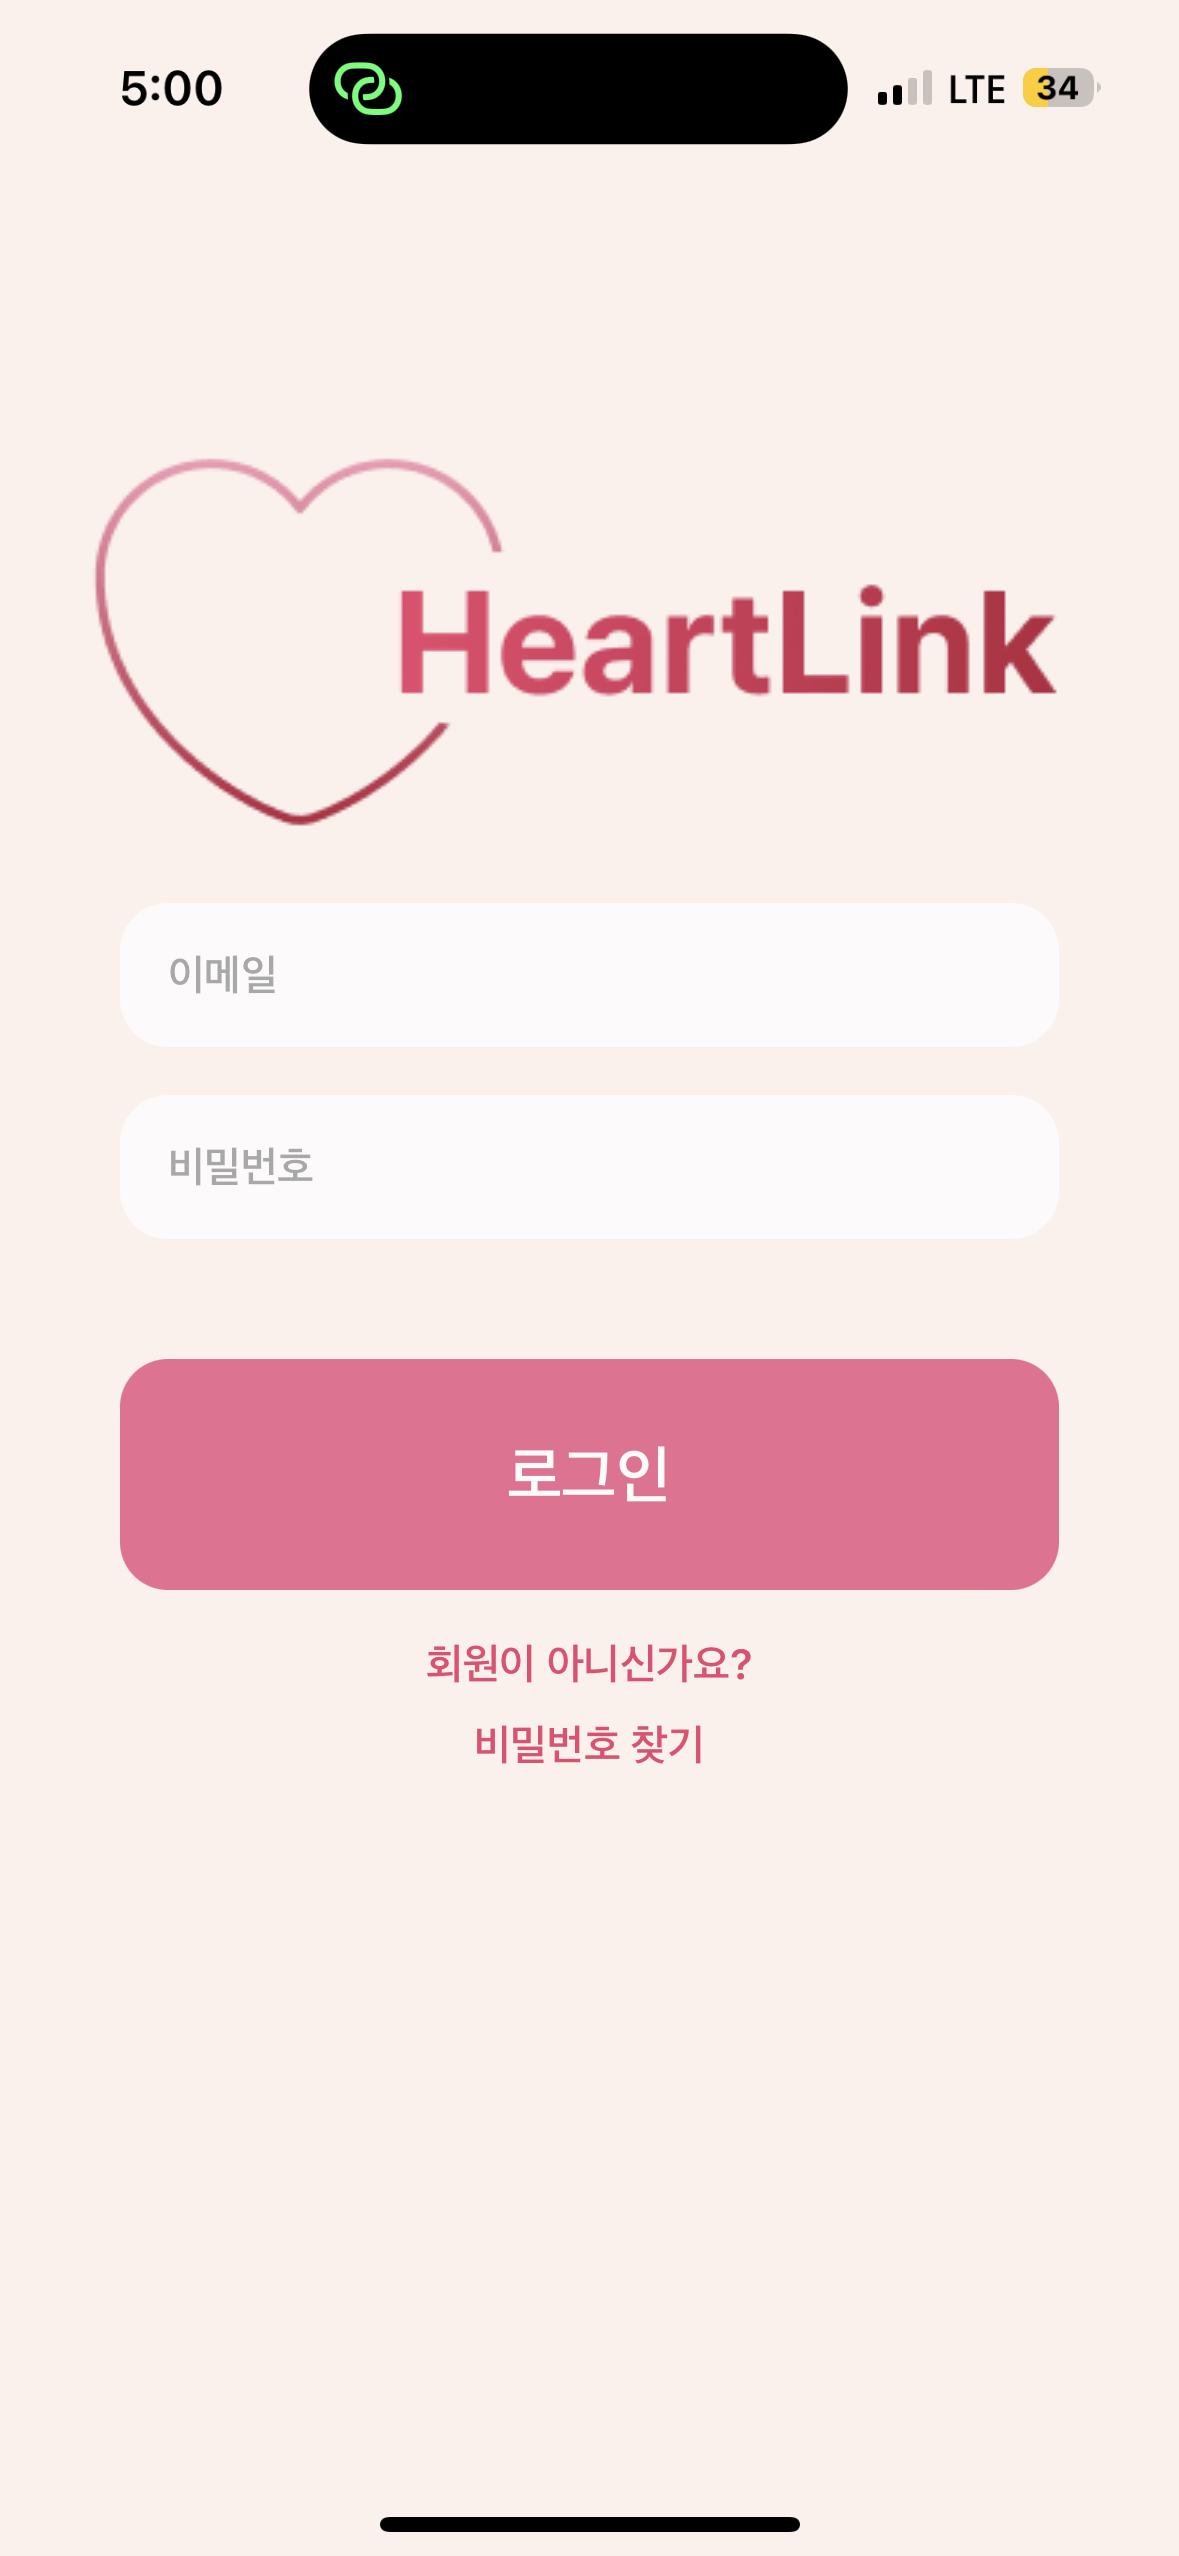
\includegraphics[width=3cm]{Images/page/login.png}}
            \caption{Login Page}
            \label{fig}
        \end{figure}
        The login page serves as the initial entry point of the application. Without logging in, users cannot access any of the app's features. Users can log in with an existing account or create a new one if they do not already have an account.
        
        Back-End Perspective: 
        When a user submits their email and password, the client sends this data to the server's login API endpoint. The server validates the credentials against the stored user data in MongoDB. If valid, the server generates a JWT token using the user's ID and secret key. This token is returned to the client for authentication purposes and has an expiration time for security. Session management is handled by the server, and any active tokens are stored securely. The server also supports token-based authentication for secure API interactions. 
        
        Front-End Perspective:
        The login form is built using React Native. When the user taps on the email or password input fields, the field borders are highlighted with the app's brand color, and the keyboard appears. To maintain visibility, the screen adjusts automatically when the keyboard is active. Input validation ensures both fields contain valid data before enabling the login button. Upon pressing the login button, the app sends the credentials to the server and displays a loading state during authentication. Successful login navigates the user to the main feed of the application, while a failed login triggers an error message. The login button is disabled while the app processes the request to prevent duplicate submissions.

   \subsection{Register Page}
        \begin{figure}[htbp]
            \centerline{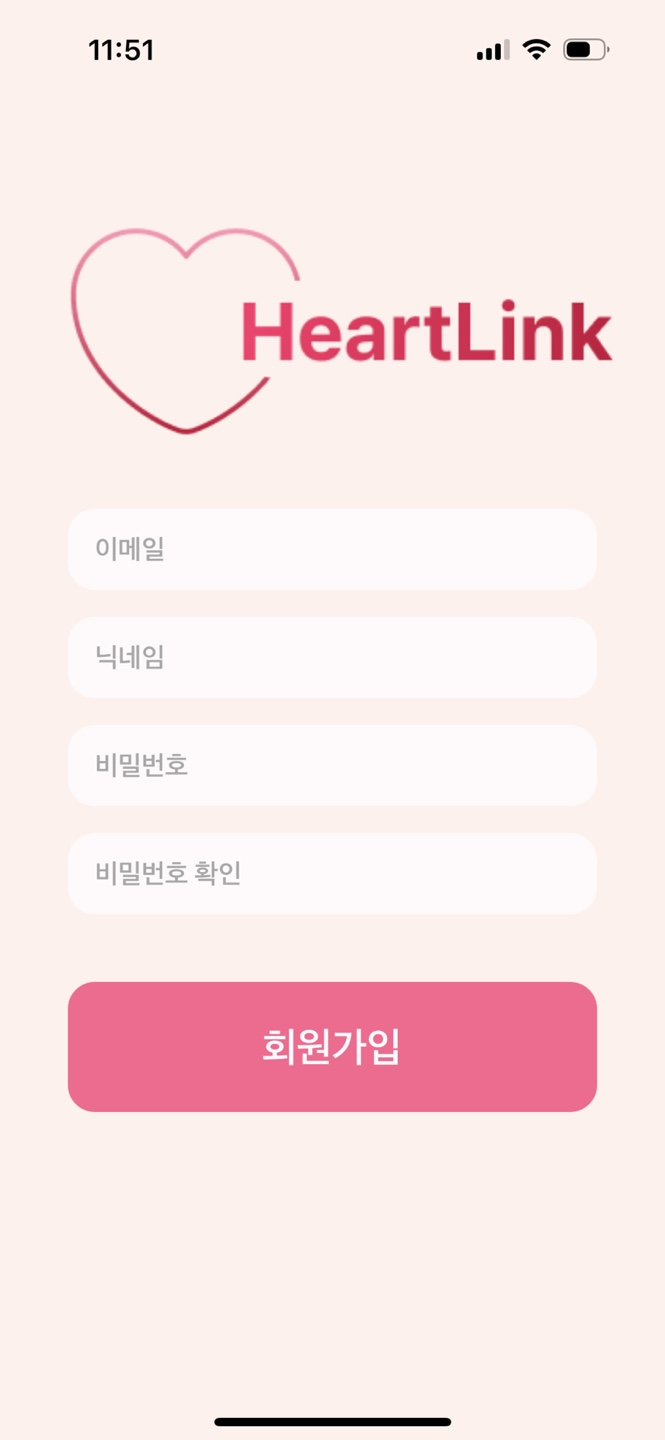
\includegraphics[width=3cm]{Images/page/register.jpg}}
            \caption{Register Page}
            \label{fig}
        \end{figure}
        The registration page allows users to create a new account by providing their email, nickname, password, and password confirmation. Users must ensure all fields are filled correctly, and the password matches the confirmation field. The password must also meet the minimum requirement of at least six characters. 
        Once the user submits the registration form, the data is sent to the server for processing. The server validates the email's uniqueness and ensures the nickname is not already in use. If all validations pass, the user data is securely stored, and the user is redirected to the login page. 
        The registration form is designed with React Native, featuring a clean and user-friendly interface. The registration button remains inactive until all fields are properly filled. During the registration process, a loading state is displayed to indicate progress. If the registration fails, an alert message informs the user of the issue, allowing them to make corrections and try again. 
        The page is styled consistently with the app's branding, maintaining a seamless user experience from registration to login.

   \subsection{MainFeed Page}
        \begin{figure}[htbp]
            \centerline{\includegraphics[width=3cm]{Images/page/feed.png}}
            \caption{MainFeed Page}
            \label{fig}
        \end{figure}
        The dashboard page is the main feed page (main page) that is first shown to users after login succeeds. The main function of the dashboard page is showing all of the friends' real-time latest posts. To help this objective, users can infinitely scroll down the page. Also the user can delete or revise the post through the delete/revise button on the top-right side of the post.

        These two buttons are basically invisible, but only the post owner can see them. And the emotion emojis below the post content are the emotions for the users can select his/her own daily mood. The only selected emotion is shown as opacity 100\% and the others are as transparency 50\%. These data can be sourced from the MongoDB database and the AWS S3 cloud then shown to the users.

        At the bottom of the screen, there is a menu bar that can lead user to another screen and functions. For the main menu bar, there are AI-CLOI, AI-album, main feed, friend list, and my page. At the top of the screen, if the user presses the middle '—' button, the screen is transited to the group selection screen.

        It's a screen composed of tabs, and from the user's perspective, it's not ideal to send requests every time you switch tabs, as it can cause delays. Therefore, as soon as user enters this screen, all the data is fetched all at once. This data is stored in a context for later use.

    \subsection{Friend Page}
        \begin{figure}[htbp]
            \centerline{
            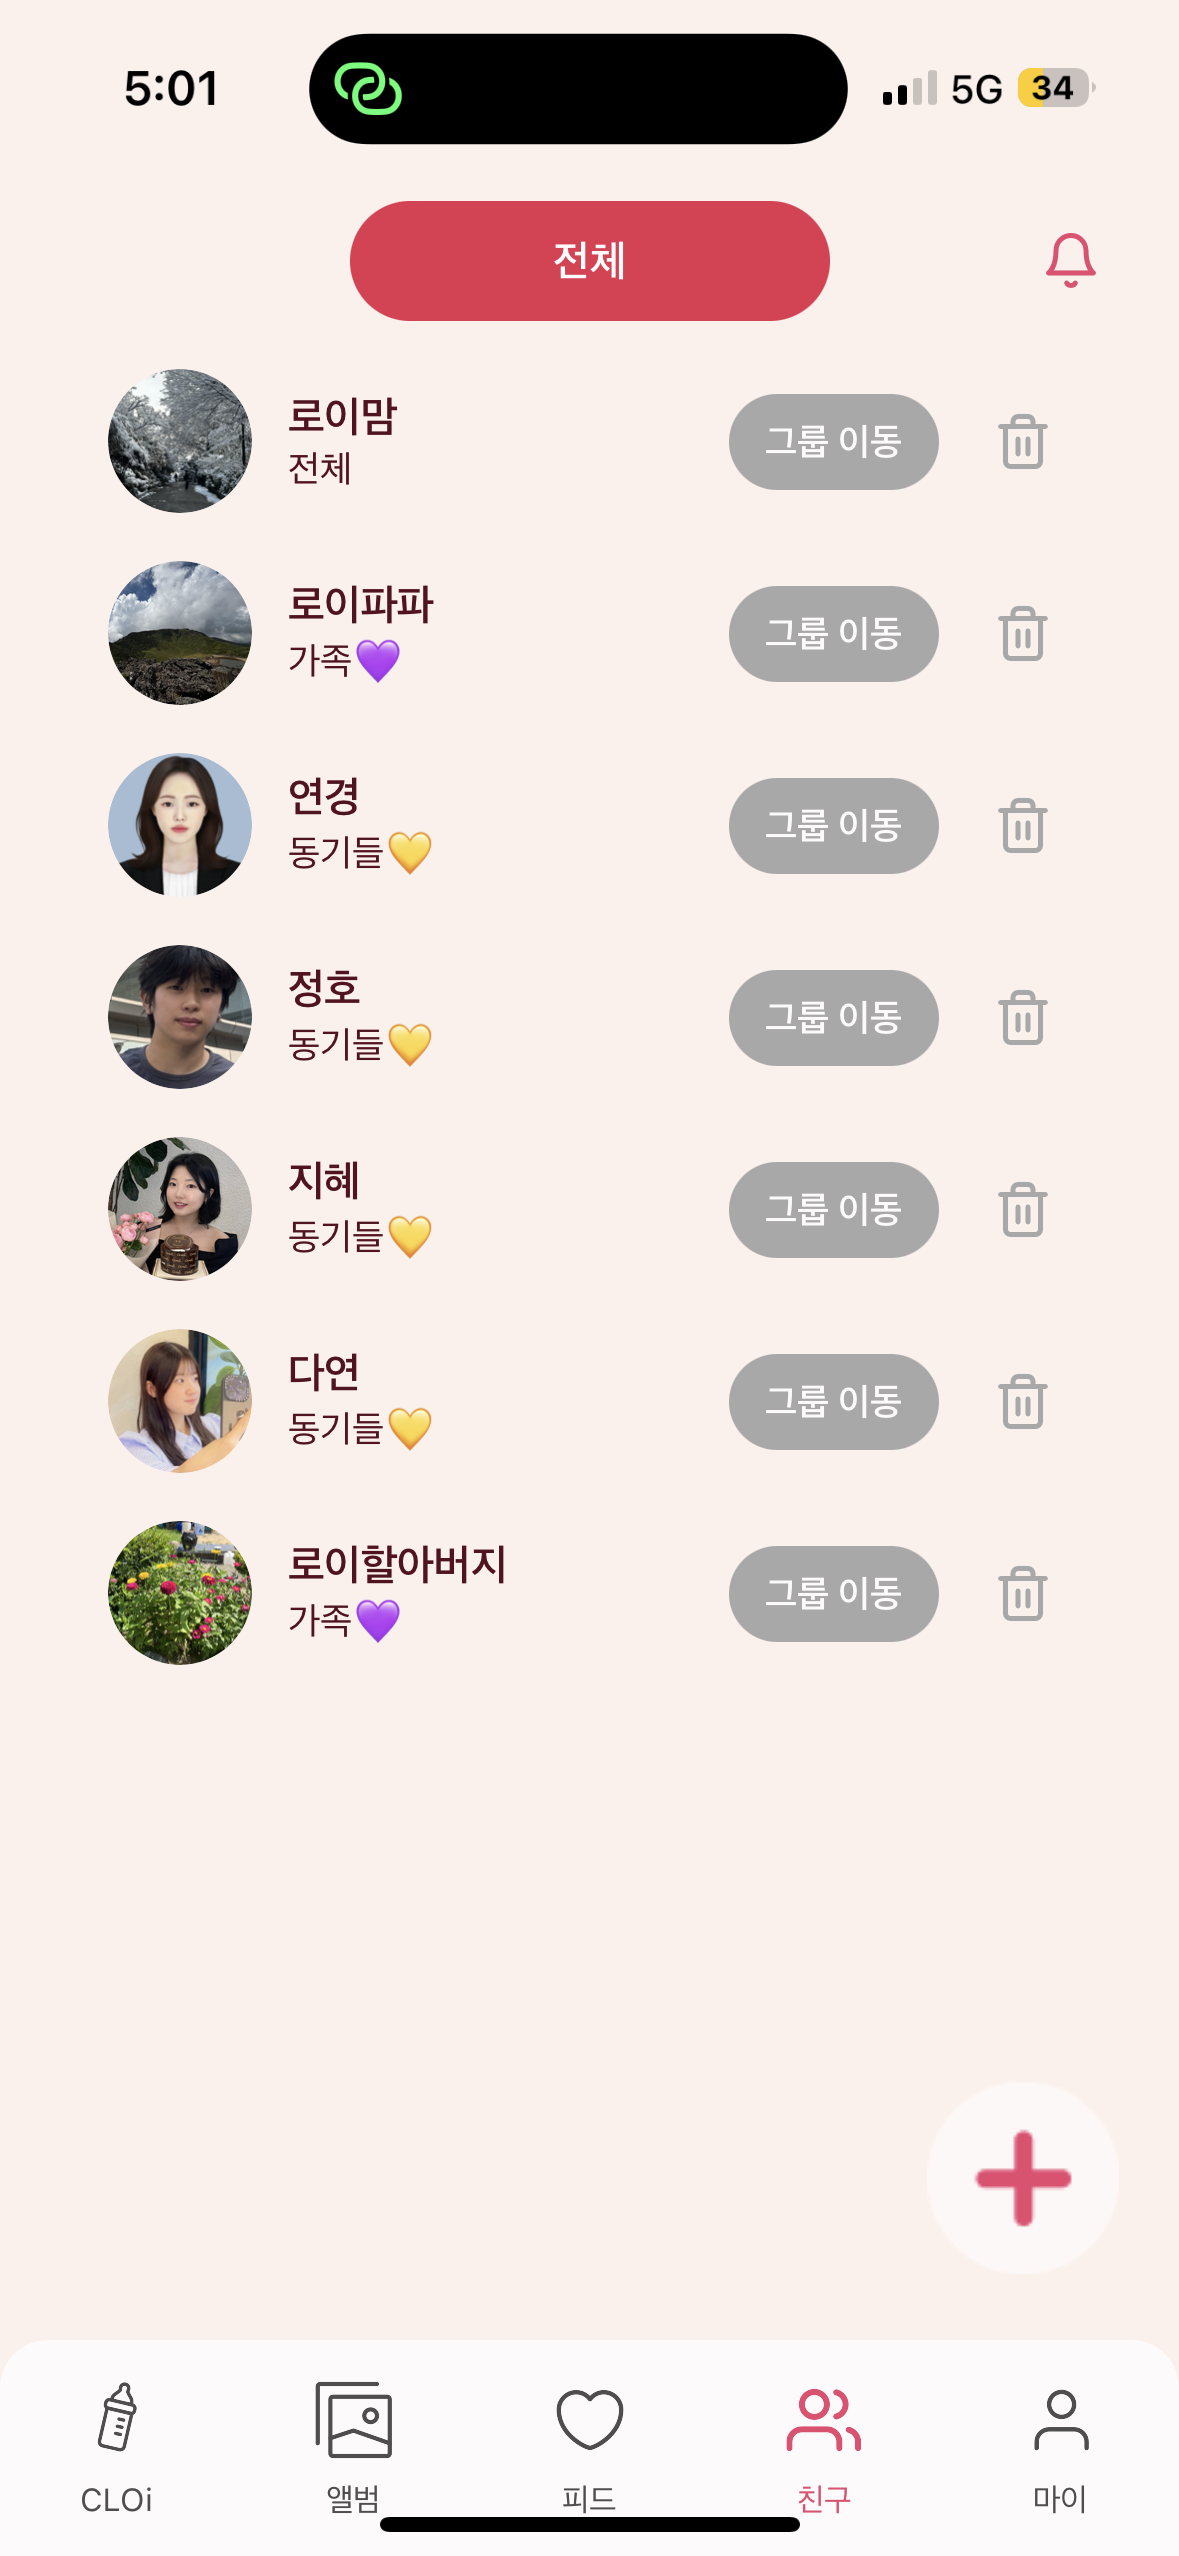
\includegraphics[width=3cm]{Images/page/friends.png}
            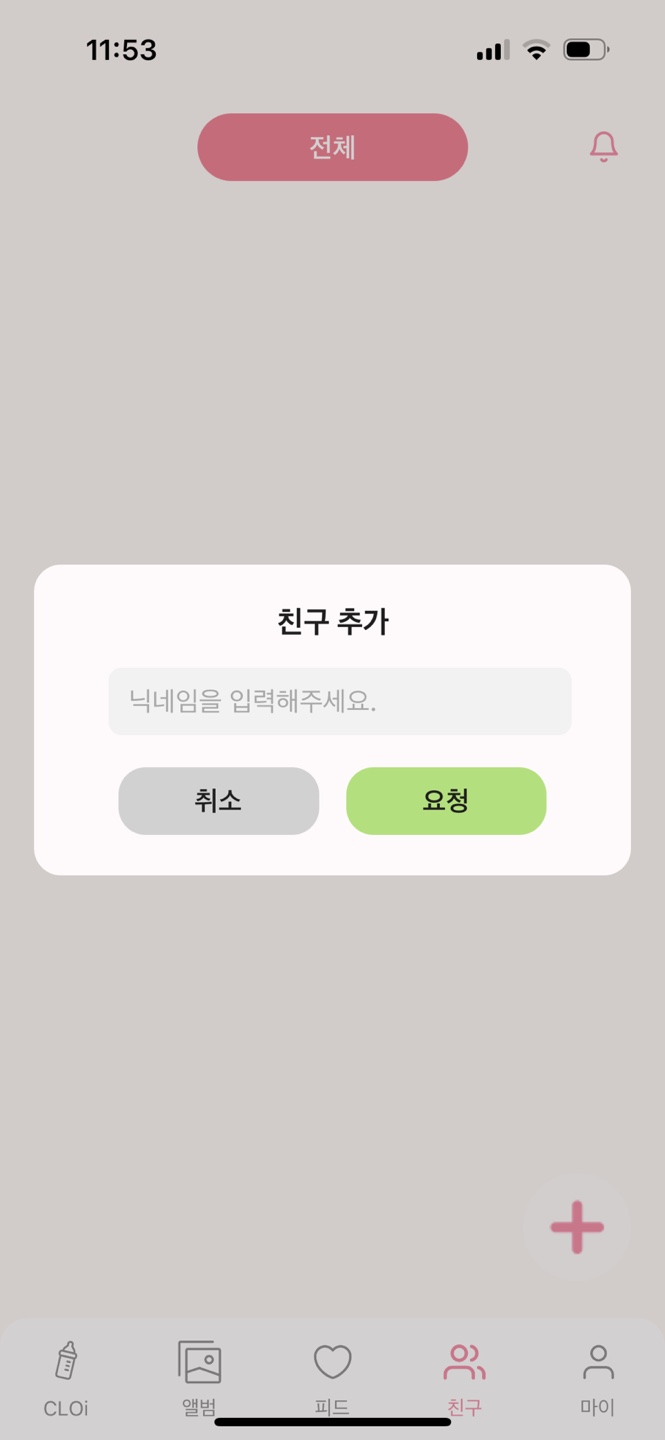
\includegraphics[width=3cm]{Images/page/addFriend.jpg}}
            \caption{Friend Page}
            \label{fig}
        \end{figure}
        To share the posts with other users, a user should add other users as 'friend'. The friend means they can make a group and can see their posts each other. If a user presses the 'friend' tab in the main menu bar, the friend list screen is shown and the user can search for the users through the add (+) button in the right-bottom side of the screen.

        Users can search for other users by his/her nickname. Then after user1 adds user2 as friend, the friend request message is sent to the user2. User2 can see this message through the notification function. If the user2 accepts, they be 'friend' from that time. In the friend list, if the user presses the trash can icon button, the user can delete the selected user from friend list.

     \subsection{Group Page}
        \begin{figure}[htbp]
            \centerline{
            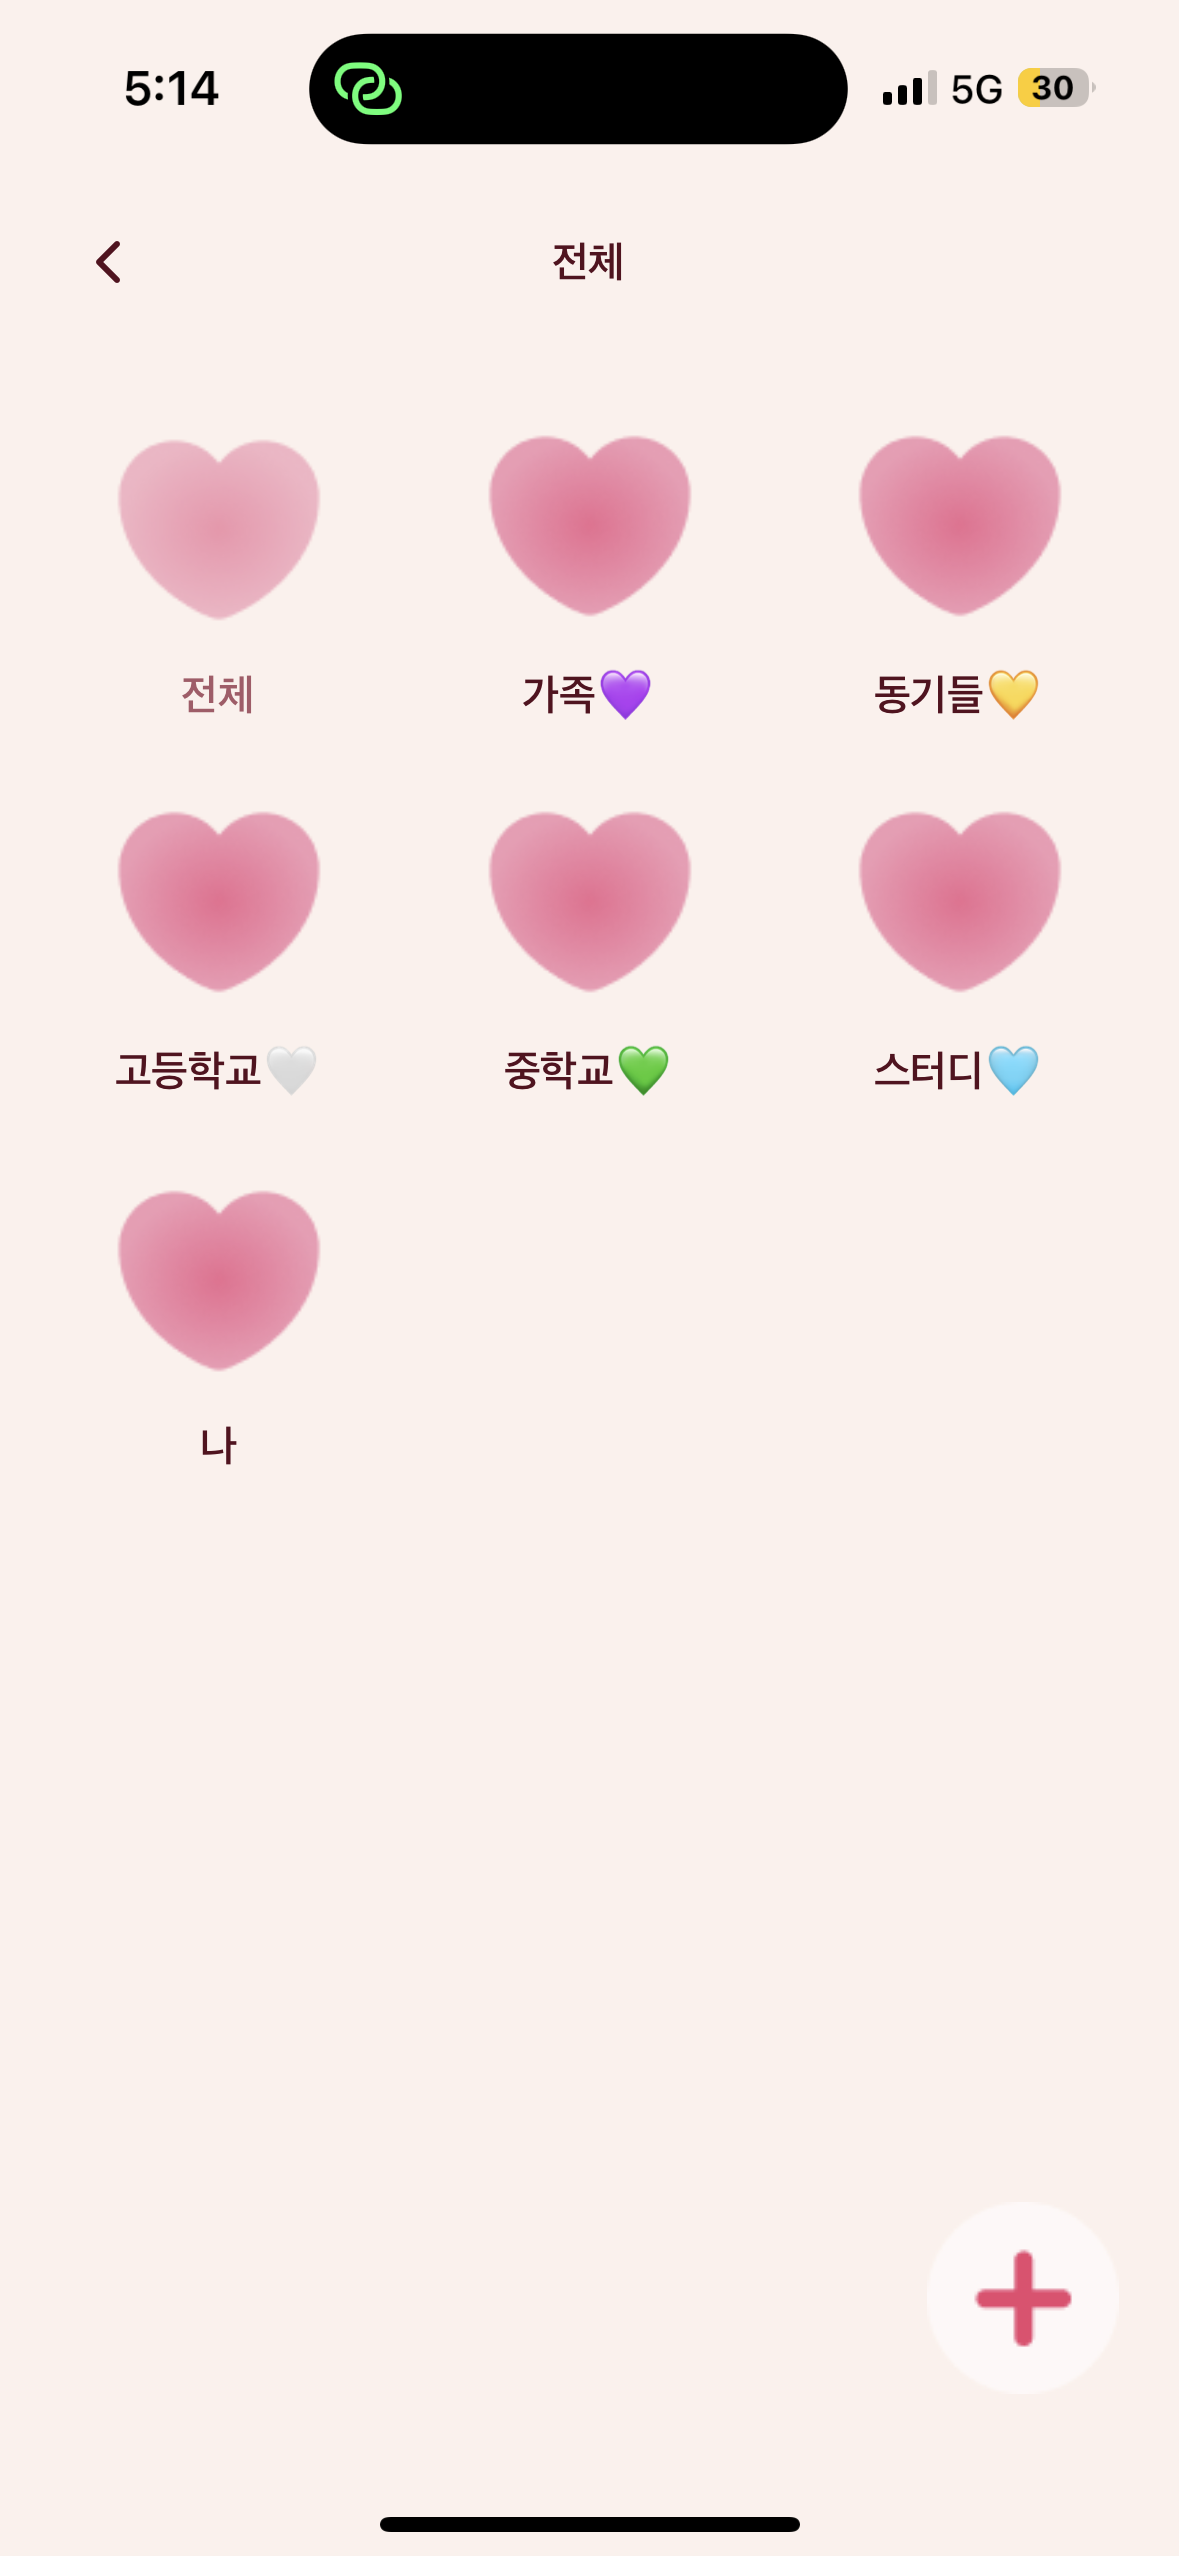
\includegraphics[width=3cm]{Images/page/group.png}
            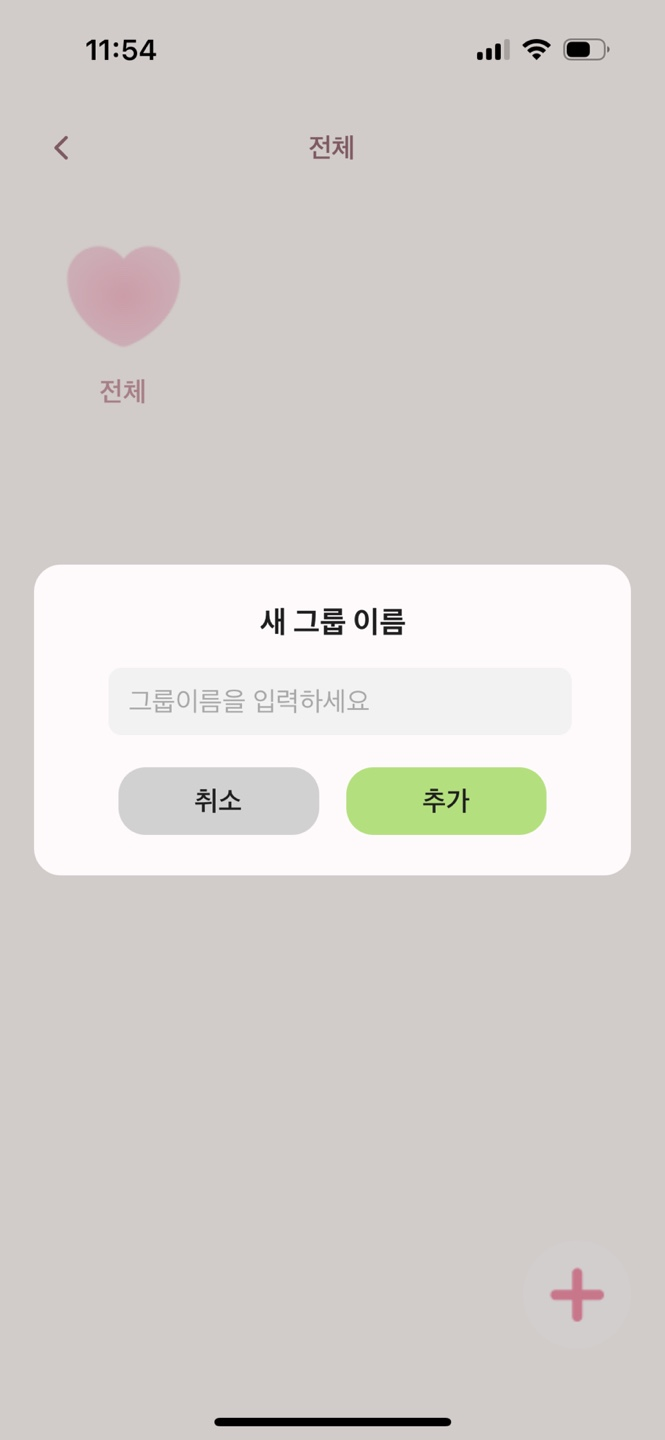
\includegraphics[width=3cm]{Images/page/addGroup.jpg}}
             \caption{Group Page}
            \label{fig}
        \end{figure}
        In the group list screen, if user can presses group for a long time, the user can change group name, and if he/she just tab once, the group member list is shown. If the user want to delete a member, then he/she can do this through trash can icon. 

        If a user presses the '—' button at the top of the main feed page, all of the group list page is shown to users. If the user presses the trash icon button in the friend list, the selected user is deleted from the friend list. The add (+) button in the right-bottom side is group creation button. If a user presses it, the group name input pop up is shown and the user can make a new group. The group name must be up to 6 Korean letters and the "Group name must be up to 6 letters." error message is shown in pop up if the size is over 6 letters. Successfully making group name, the screen is transited to friend list screen, and the user can add friends to the group or change group to another.

    \subsection{Feed Upload Page - AI Voice Recognition}
        \begin{figure}[htbp]
            \centerline{
            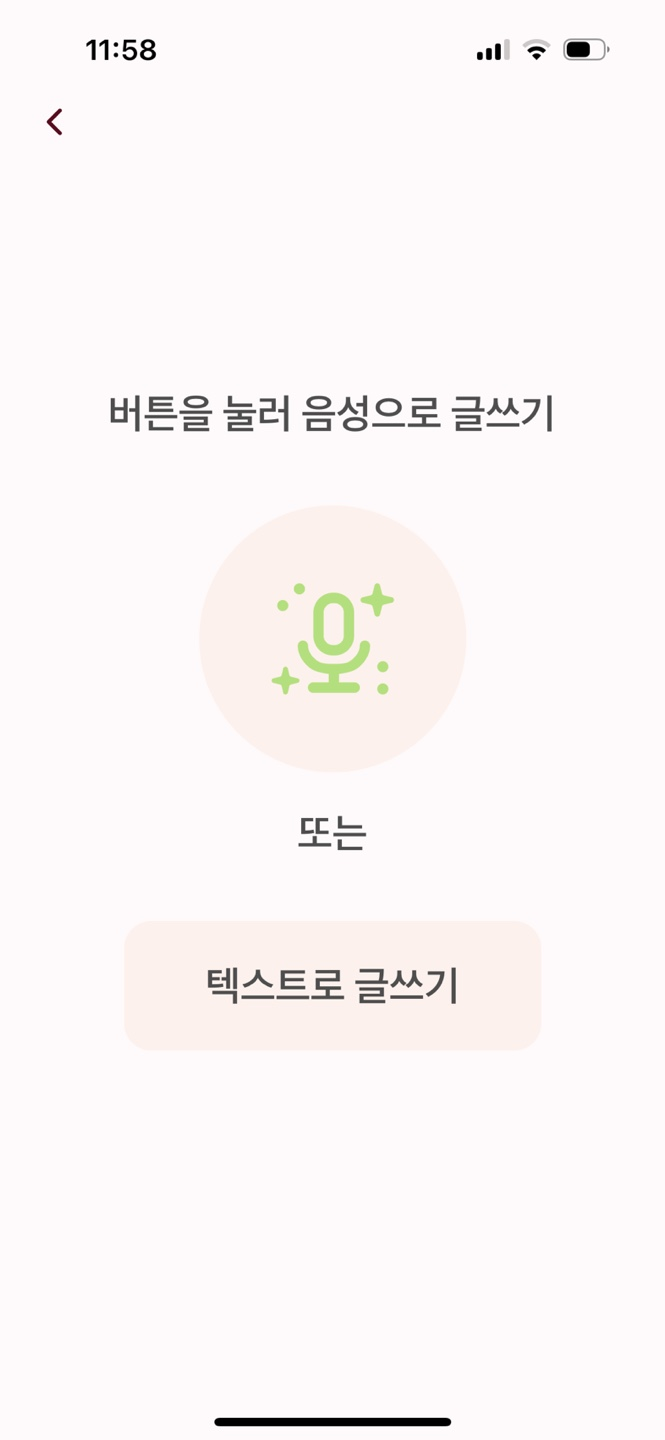
\includegraphics[width=3cm]{Images/page/recording1.jpg}
            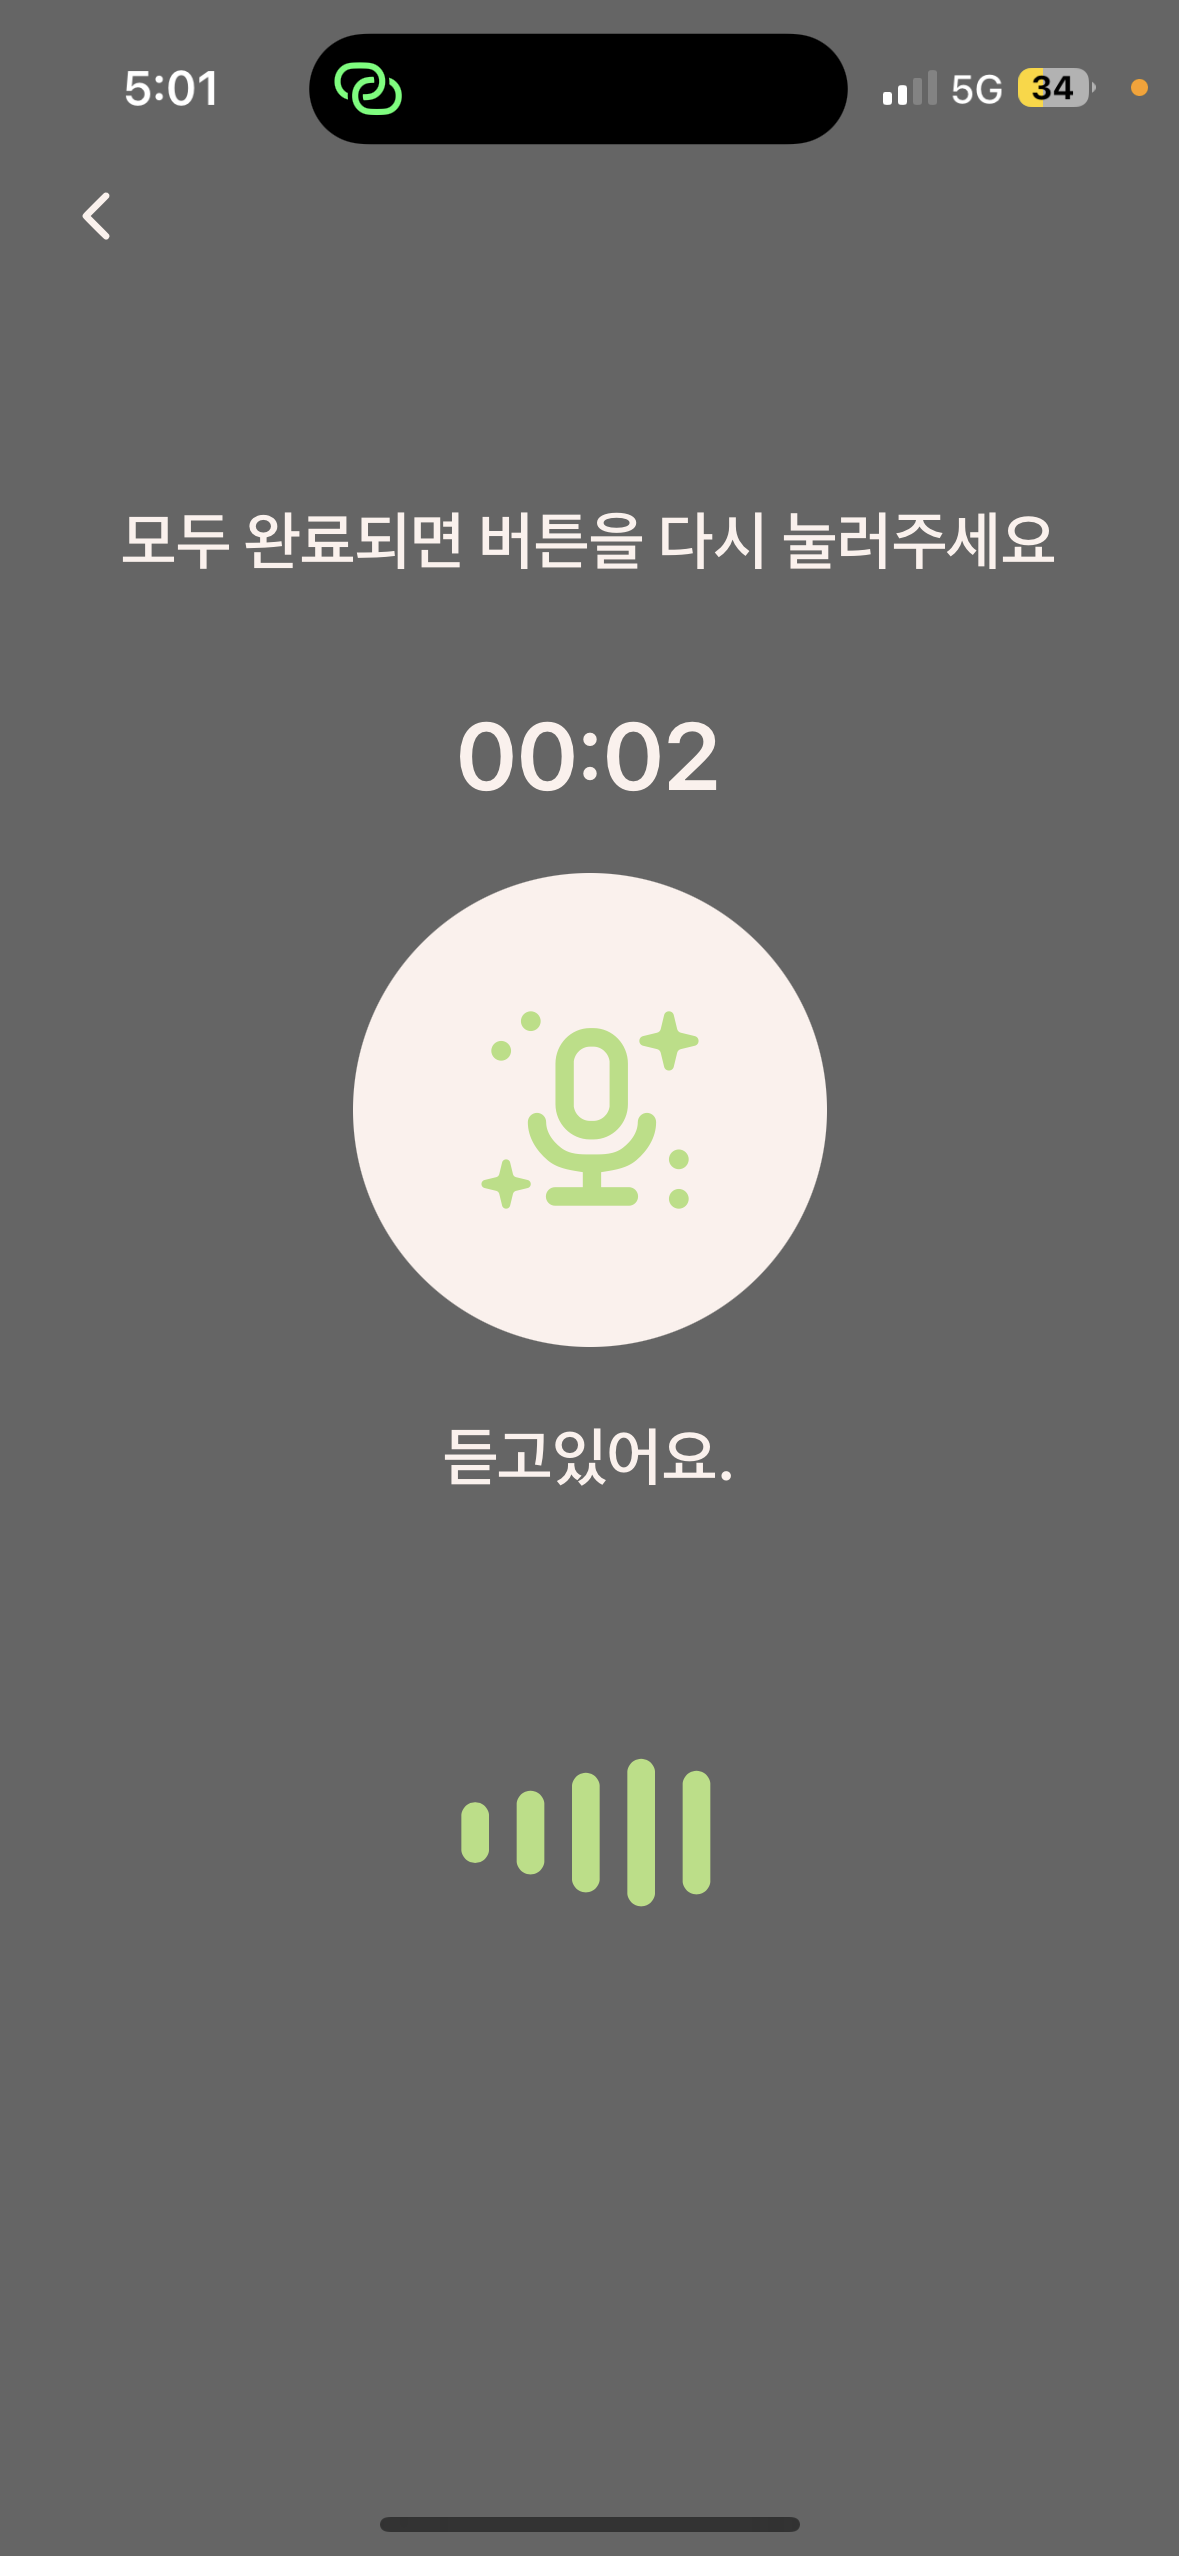
\includegraphics[width=3cm]{Images/page/recording.png}}
              \caption{Feed Upload Page - AI Voice Recognition}
            \label{fig}
        \end{figure}
        In the feed upload process of the application, users are presented with voice recognition functionality powered by OpenAI API for converting spoken words into text. When accessing the feed upload screen, users can tap the microphone button to activate the voice recognition interface, which displays a visual audio waveform animation during recording.

        The recorded voice is processed through the OpenAI API for real-time speech-to-text conversion. The interface also provides an alternative option where users can bypass the voice recognition feature and directly input text using the keyboard, offering flexibility in content creation. The text input field features a clean, minimalist design that follows the application's visual style guide created in Figma.

        When users finish speaking, the text appears on the screen. The text can be edited or modified before proceeding to the next step of adding visual content to their post.

 \subsection{Feed Upload Page - AI Image Creation}
        \begin{figure}[htbp]
            \centerline{
            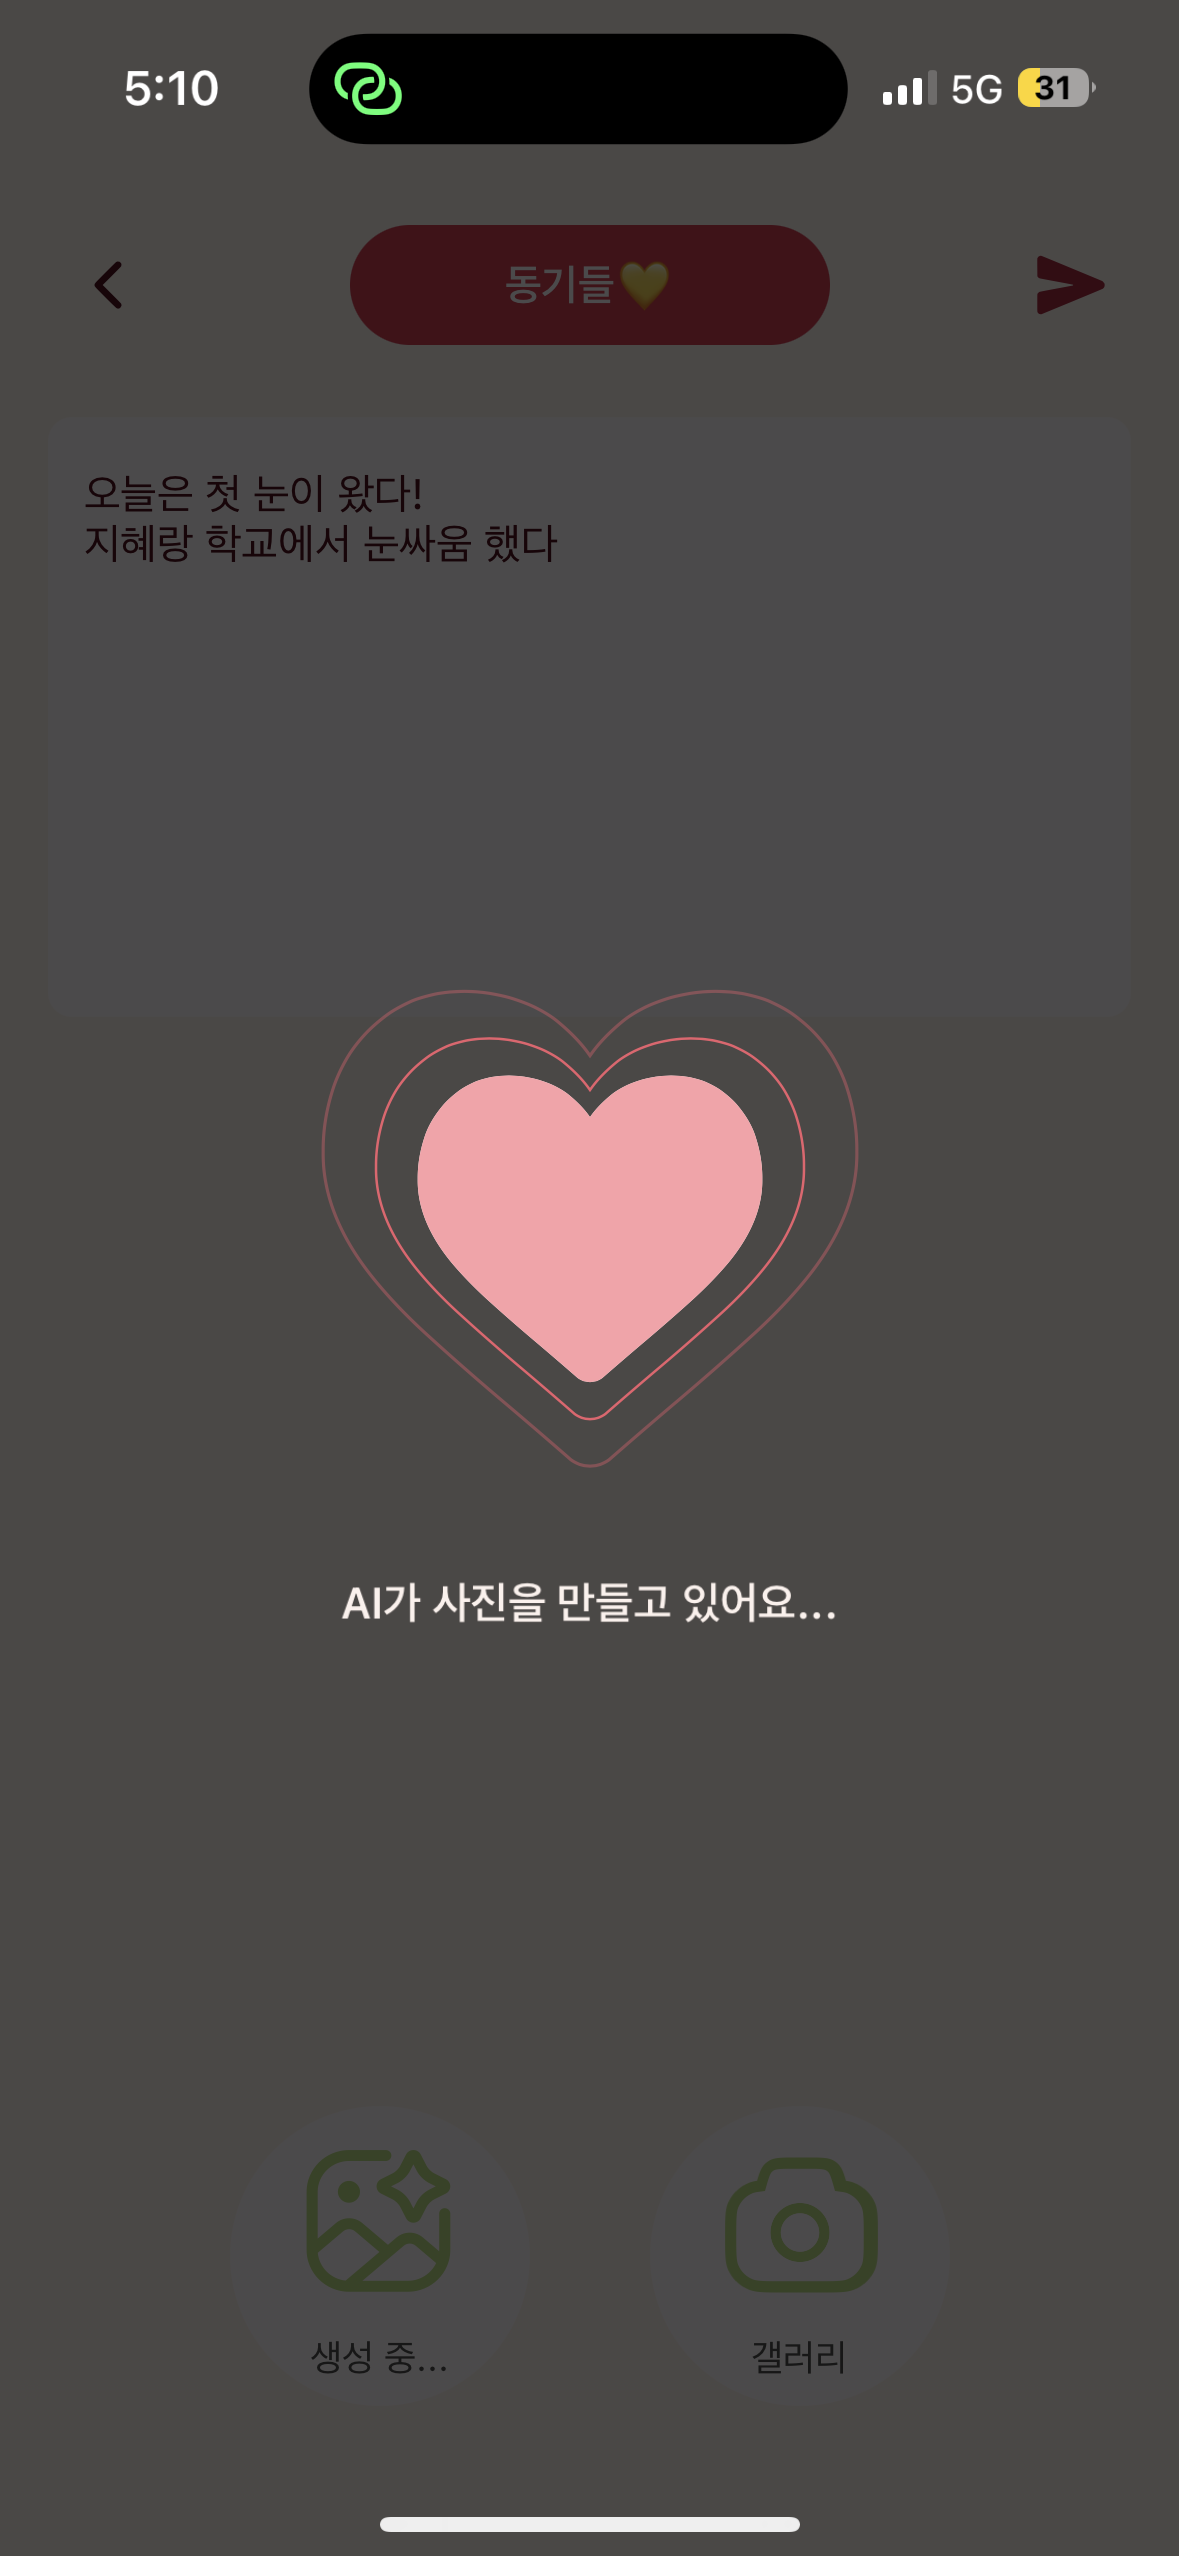
\includegraphics[width=3cm]{Images/page/creating.png}
            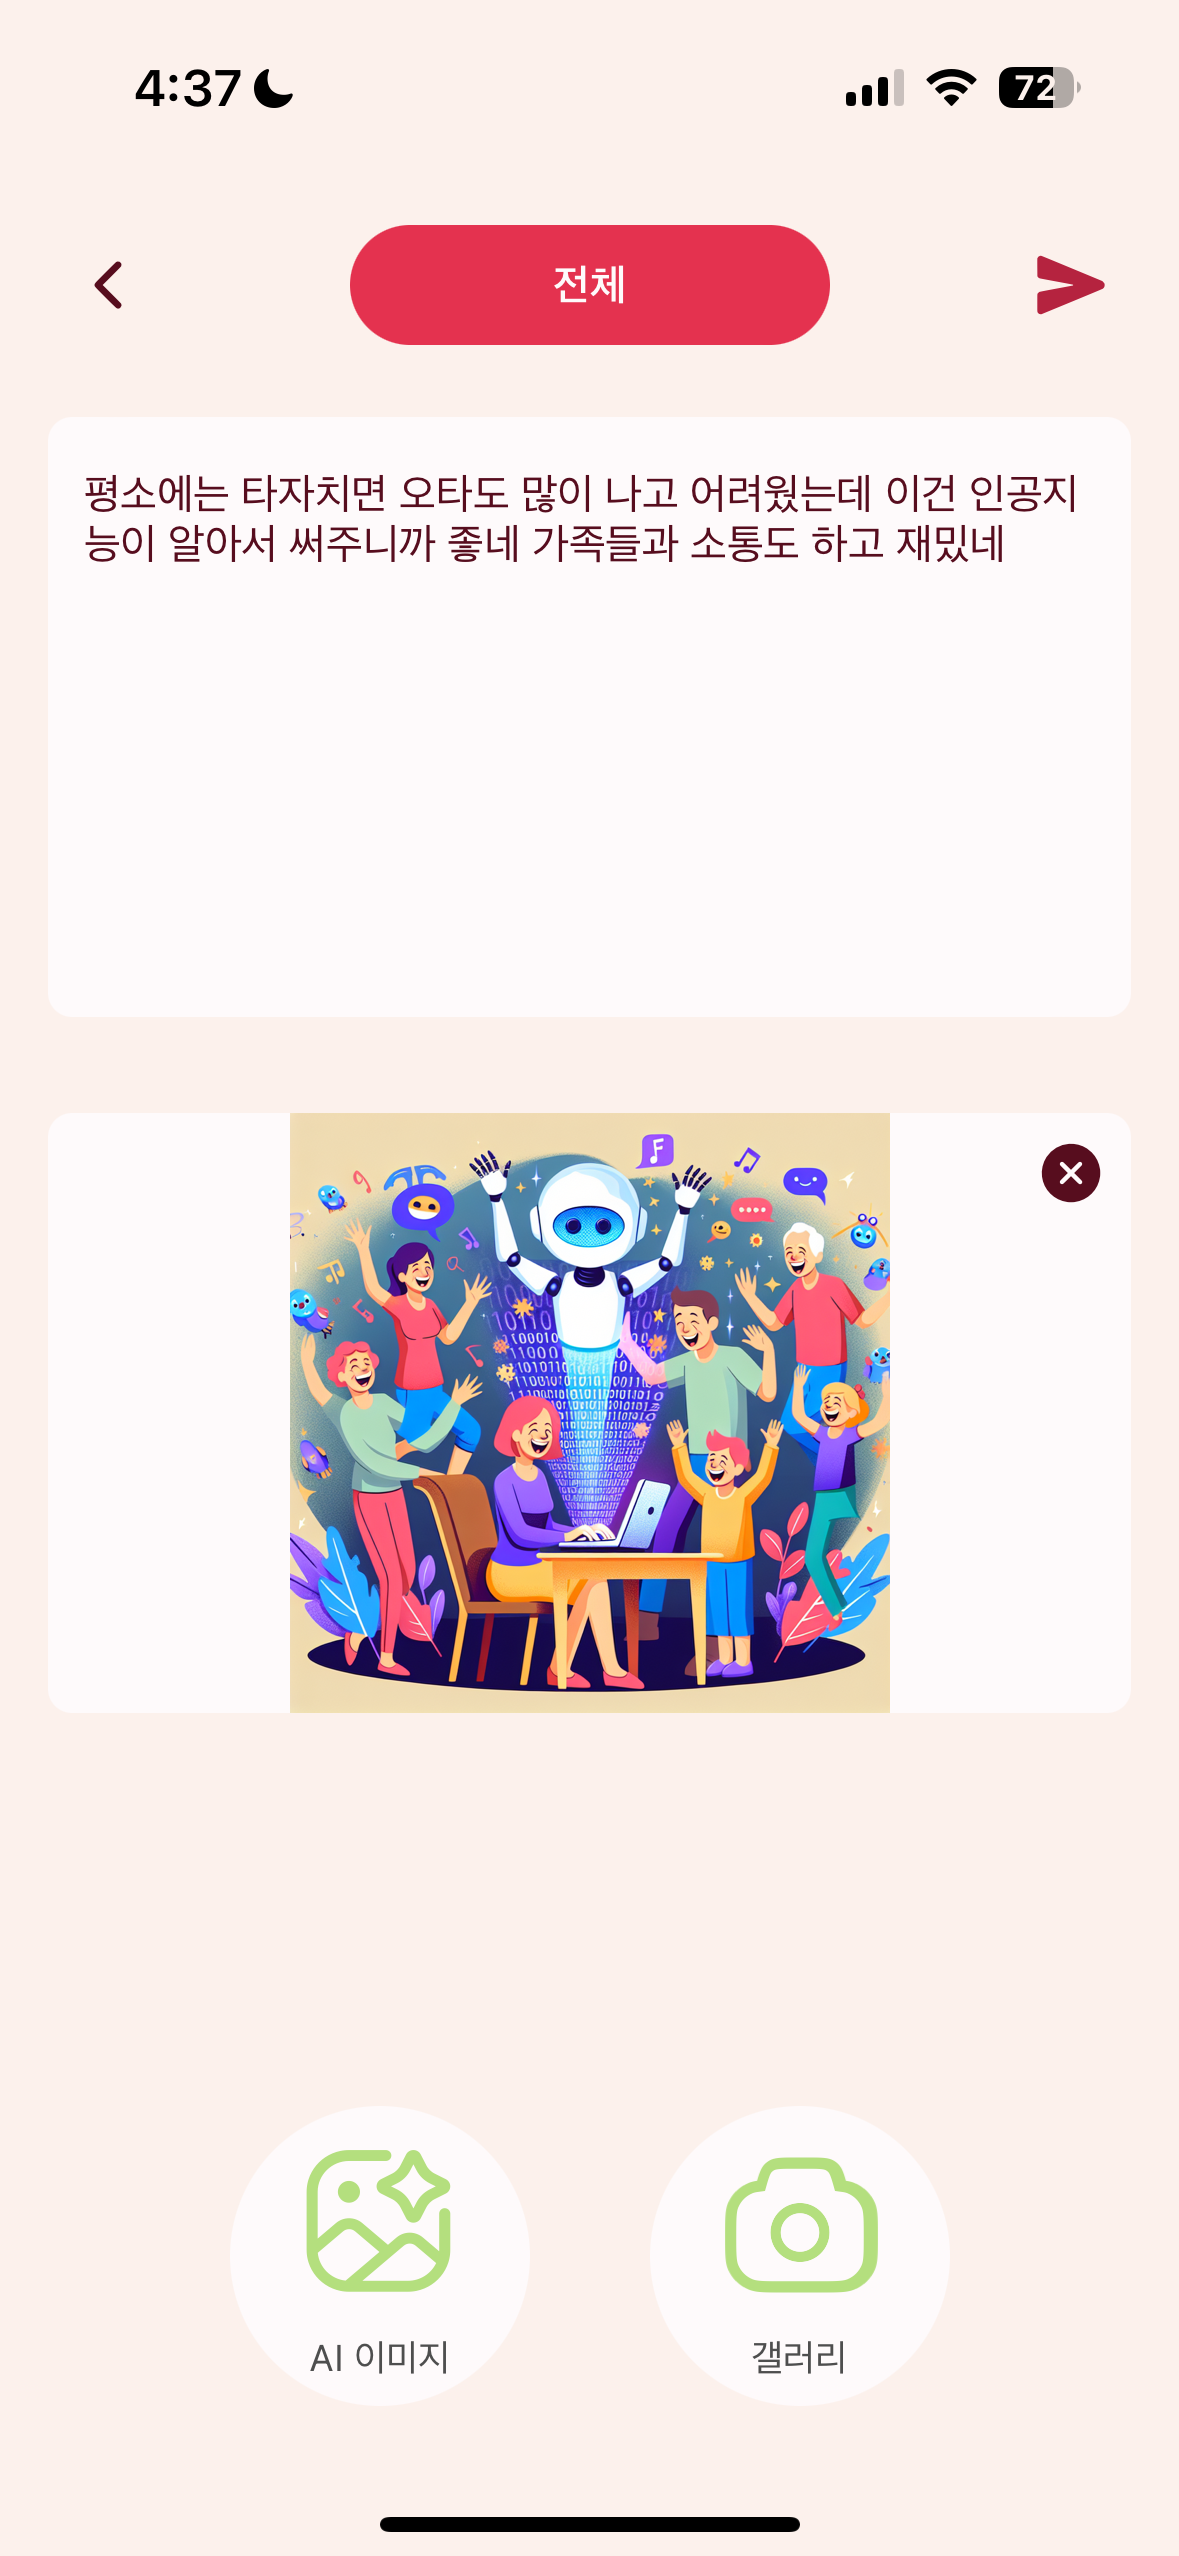
\includegraphics[width=3cm]{Images/page/writing.png}}
              \caption{Feed Upload Page - AI Image Creation}
            \label{fig}
        \end{figure}
        After obtaining the text content, either through voice recognition or manual input, the feed creation process moves to the visual content stage. Here, users are presented with two options: AI image generation or manual image selection from their gallery.

        When users choose AI image generation, the application processes the input text through an AI image generation model to create a visual representation of the text content. The generated image appears on the screen, displayed in a format optimized for the social media feed. If users are not satisfied with the initially generated image, they can tap the regenerate button to create a different variation based on the same text input.

        Alternatively, users have the option to select images directly from their device's gallery instead of using the AI-generated images. The gallery selection interface allows users to choose multiple images from their local storage. Whether using AI-generated images or manually selected ones, all visual content is stored in Amazon S3 cloud storage, while the post metadata and references are managed in MongoDB through the Express.js backend running on Amazon EC2. The entire upload process is managed through React Native's state management using Zustand, ensuring a smooth and responsive user experience throughout the content creation flow.

  \subsection{CLOi Page}
        \begin{figure}[htbp]
            \centerline{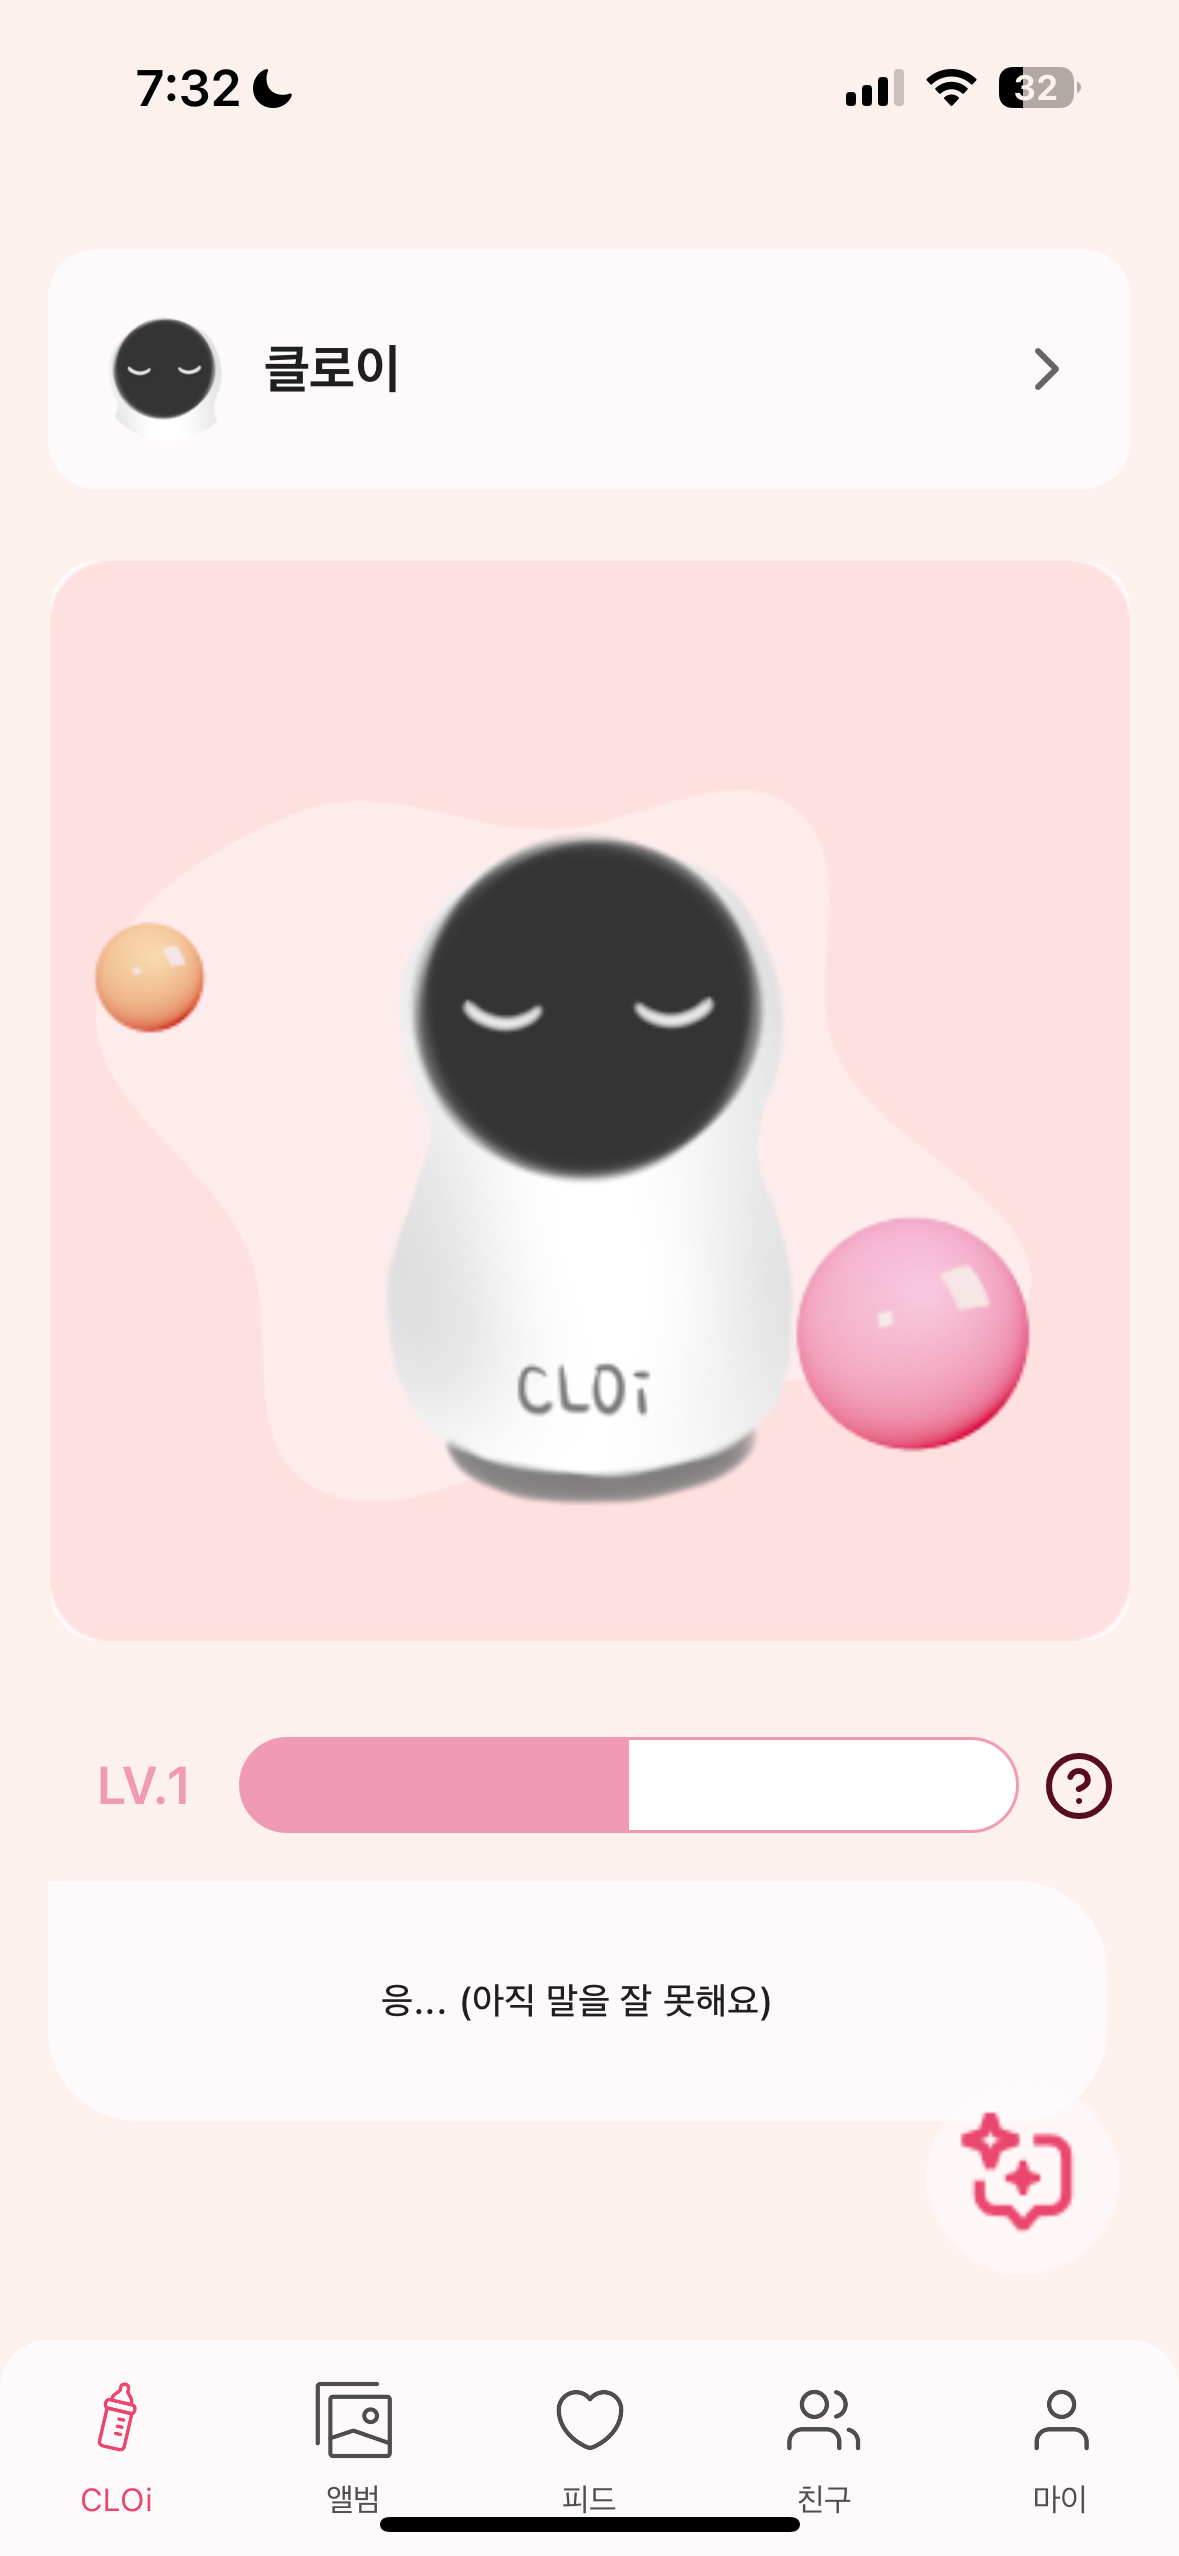
\includegraphics[width=3cm]{Images/page/cloi1.png}
            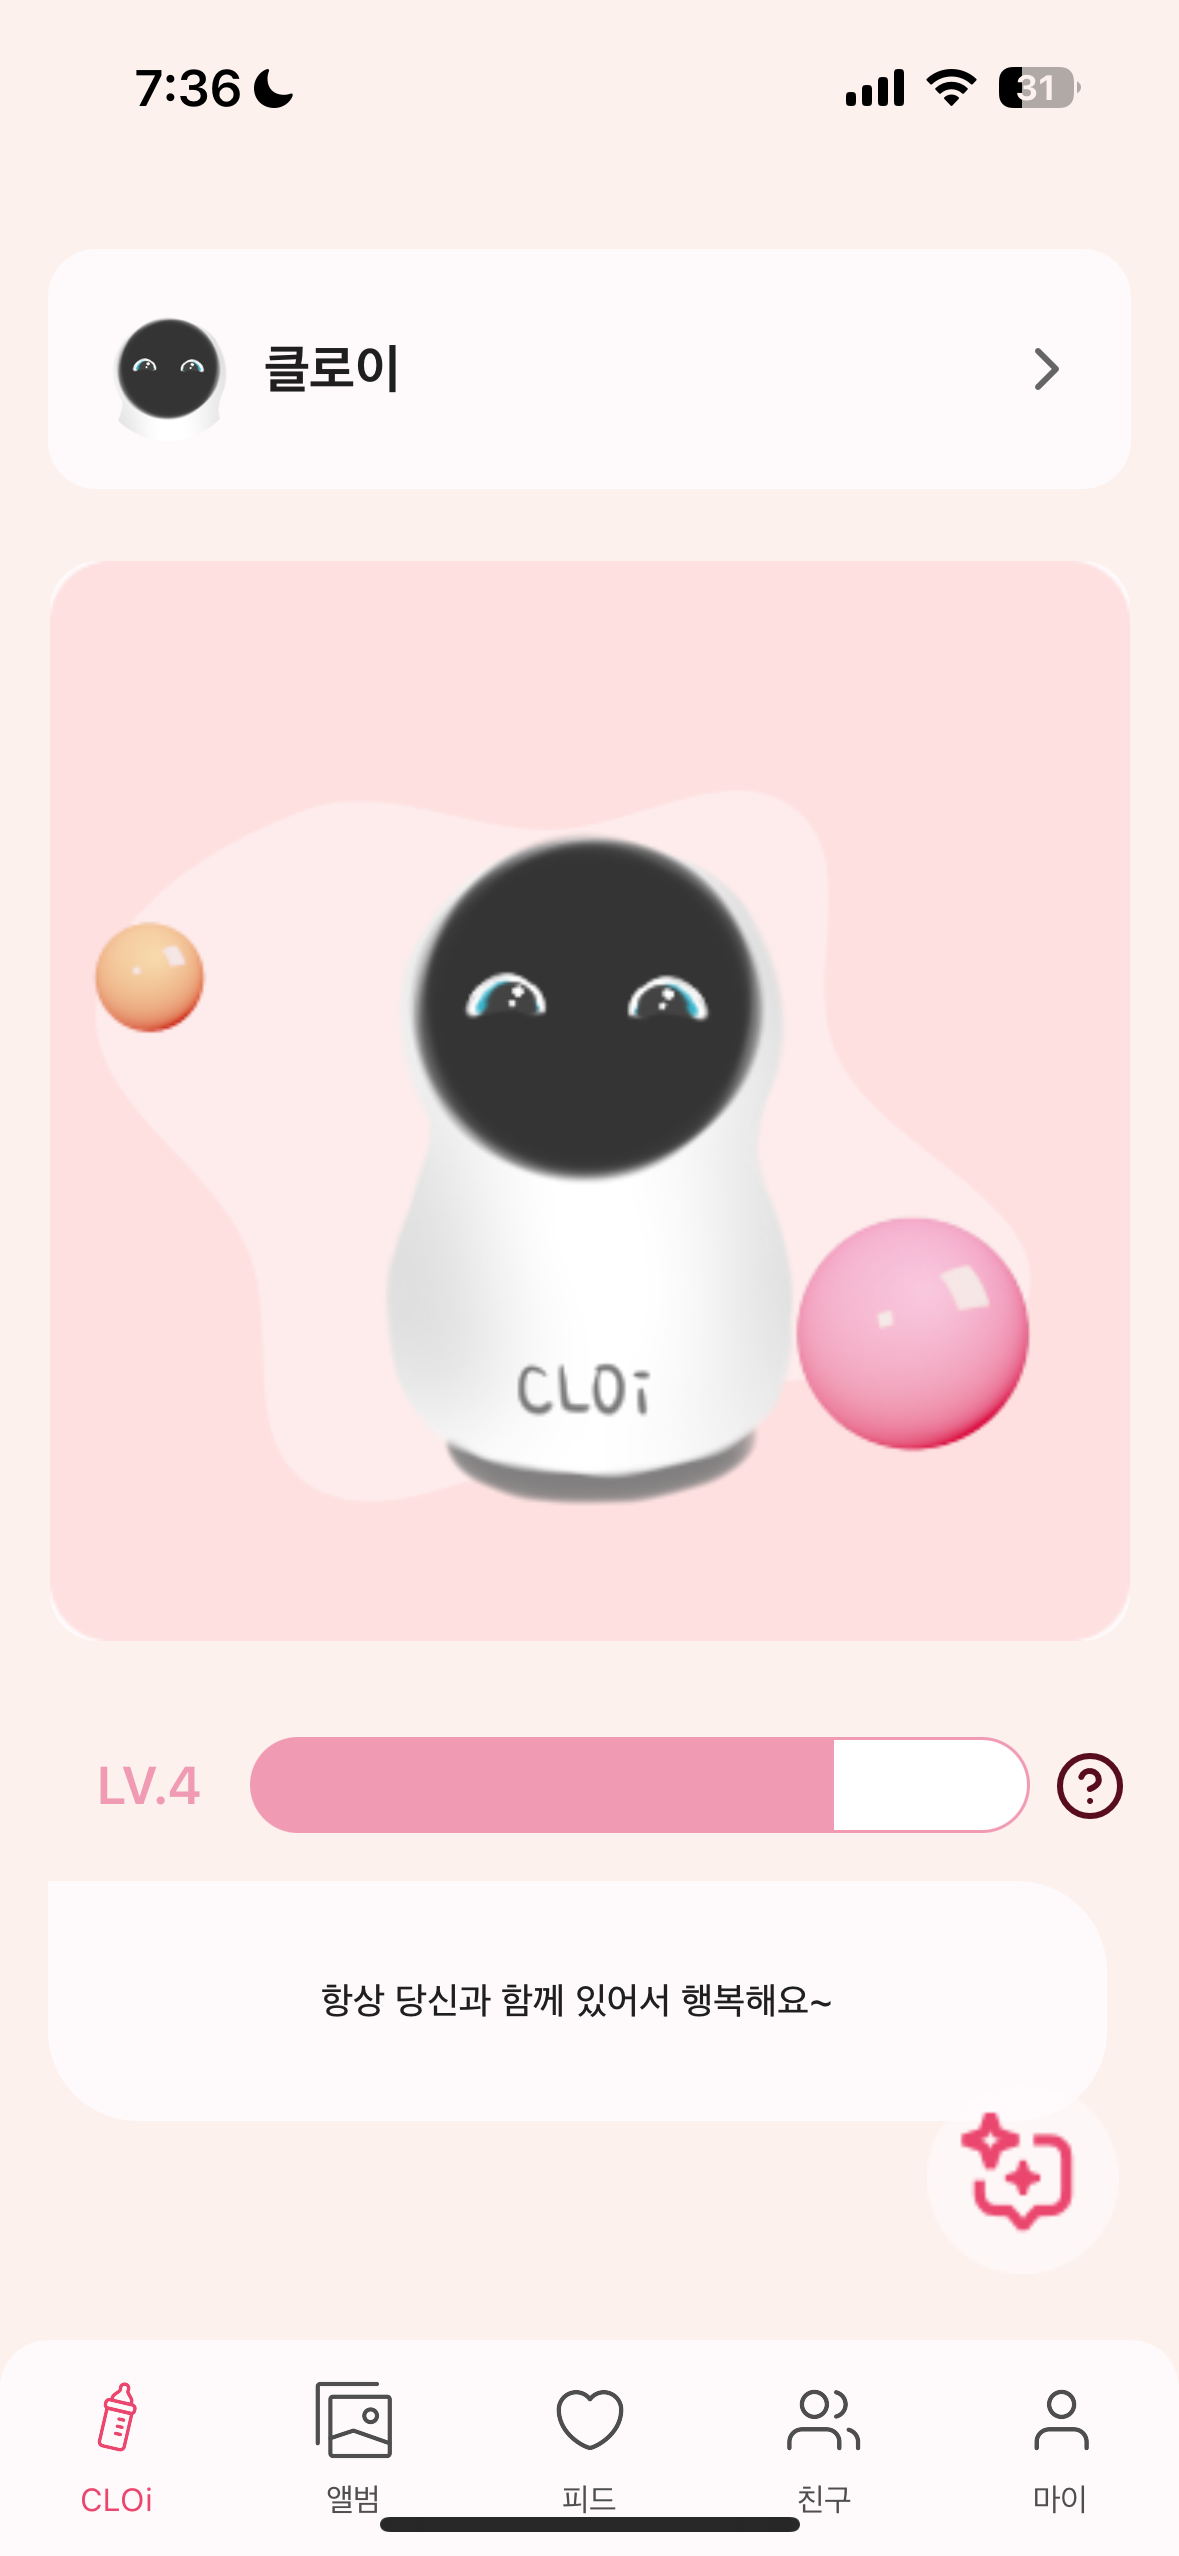
\includegraphics[width=3cm]{Images/page/cloi4.png}
            }
            \caption{CLOi Page}
            \label{fig}
        \end{figure}
        The application features an AI companion called CLOI, which grows and evolves based on user engagement and activity within the platform. CLOI starts as a baby (LV.1) and progressively grows through stages - infant (LV.2), child (LV.3), teenager (LV.4), and adult (LV.5) - as users create and share more content on the platform.

        Each evolution level of CLOI is visually represented by different facial expressions and characteristics that reflect its growth stage, creating an emotional connection with users. The evolution system is managed through the Express.js backend, which tracks the number of posts created by the user and stores the progress in MongoDB. When users reach certain posting milestones, CLOI automatically evolves to its next stage.
        
        % When users reach certain posting milestones, CLOI automatically evolves to its next stage, with the transition animated to celebrate the growth moment. CLOI also functions as an interactive AI companion that generates personalized greetings and friendly messages for users. Using the OpenAI API, CLOI analyzes the user's activity patterns, posting frequency, and time of day to create contextually appropriate and engaging messages.

        % For example, CLOI might say "I see you're working hard on creating content today!" or "It's been a while since your last post, would you like to share something new?" These interactions are designed to encourage user engagement while maintaining a friendly, supportive presence. The message generation system considers CLOI's current evolution level, ensuring that the tone and complexity of interactions match its growth stage, making the experience more authentic and emotionally resonant. The entire CLOI system is integrated into the React Native frontend using Zustand for state management, ensuring smooth animations and transitions between different states and messages.

        

\subsection{Chatbot Page}
        \begin{figure}[htbp]
            \centerline{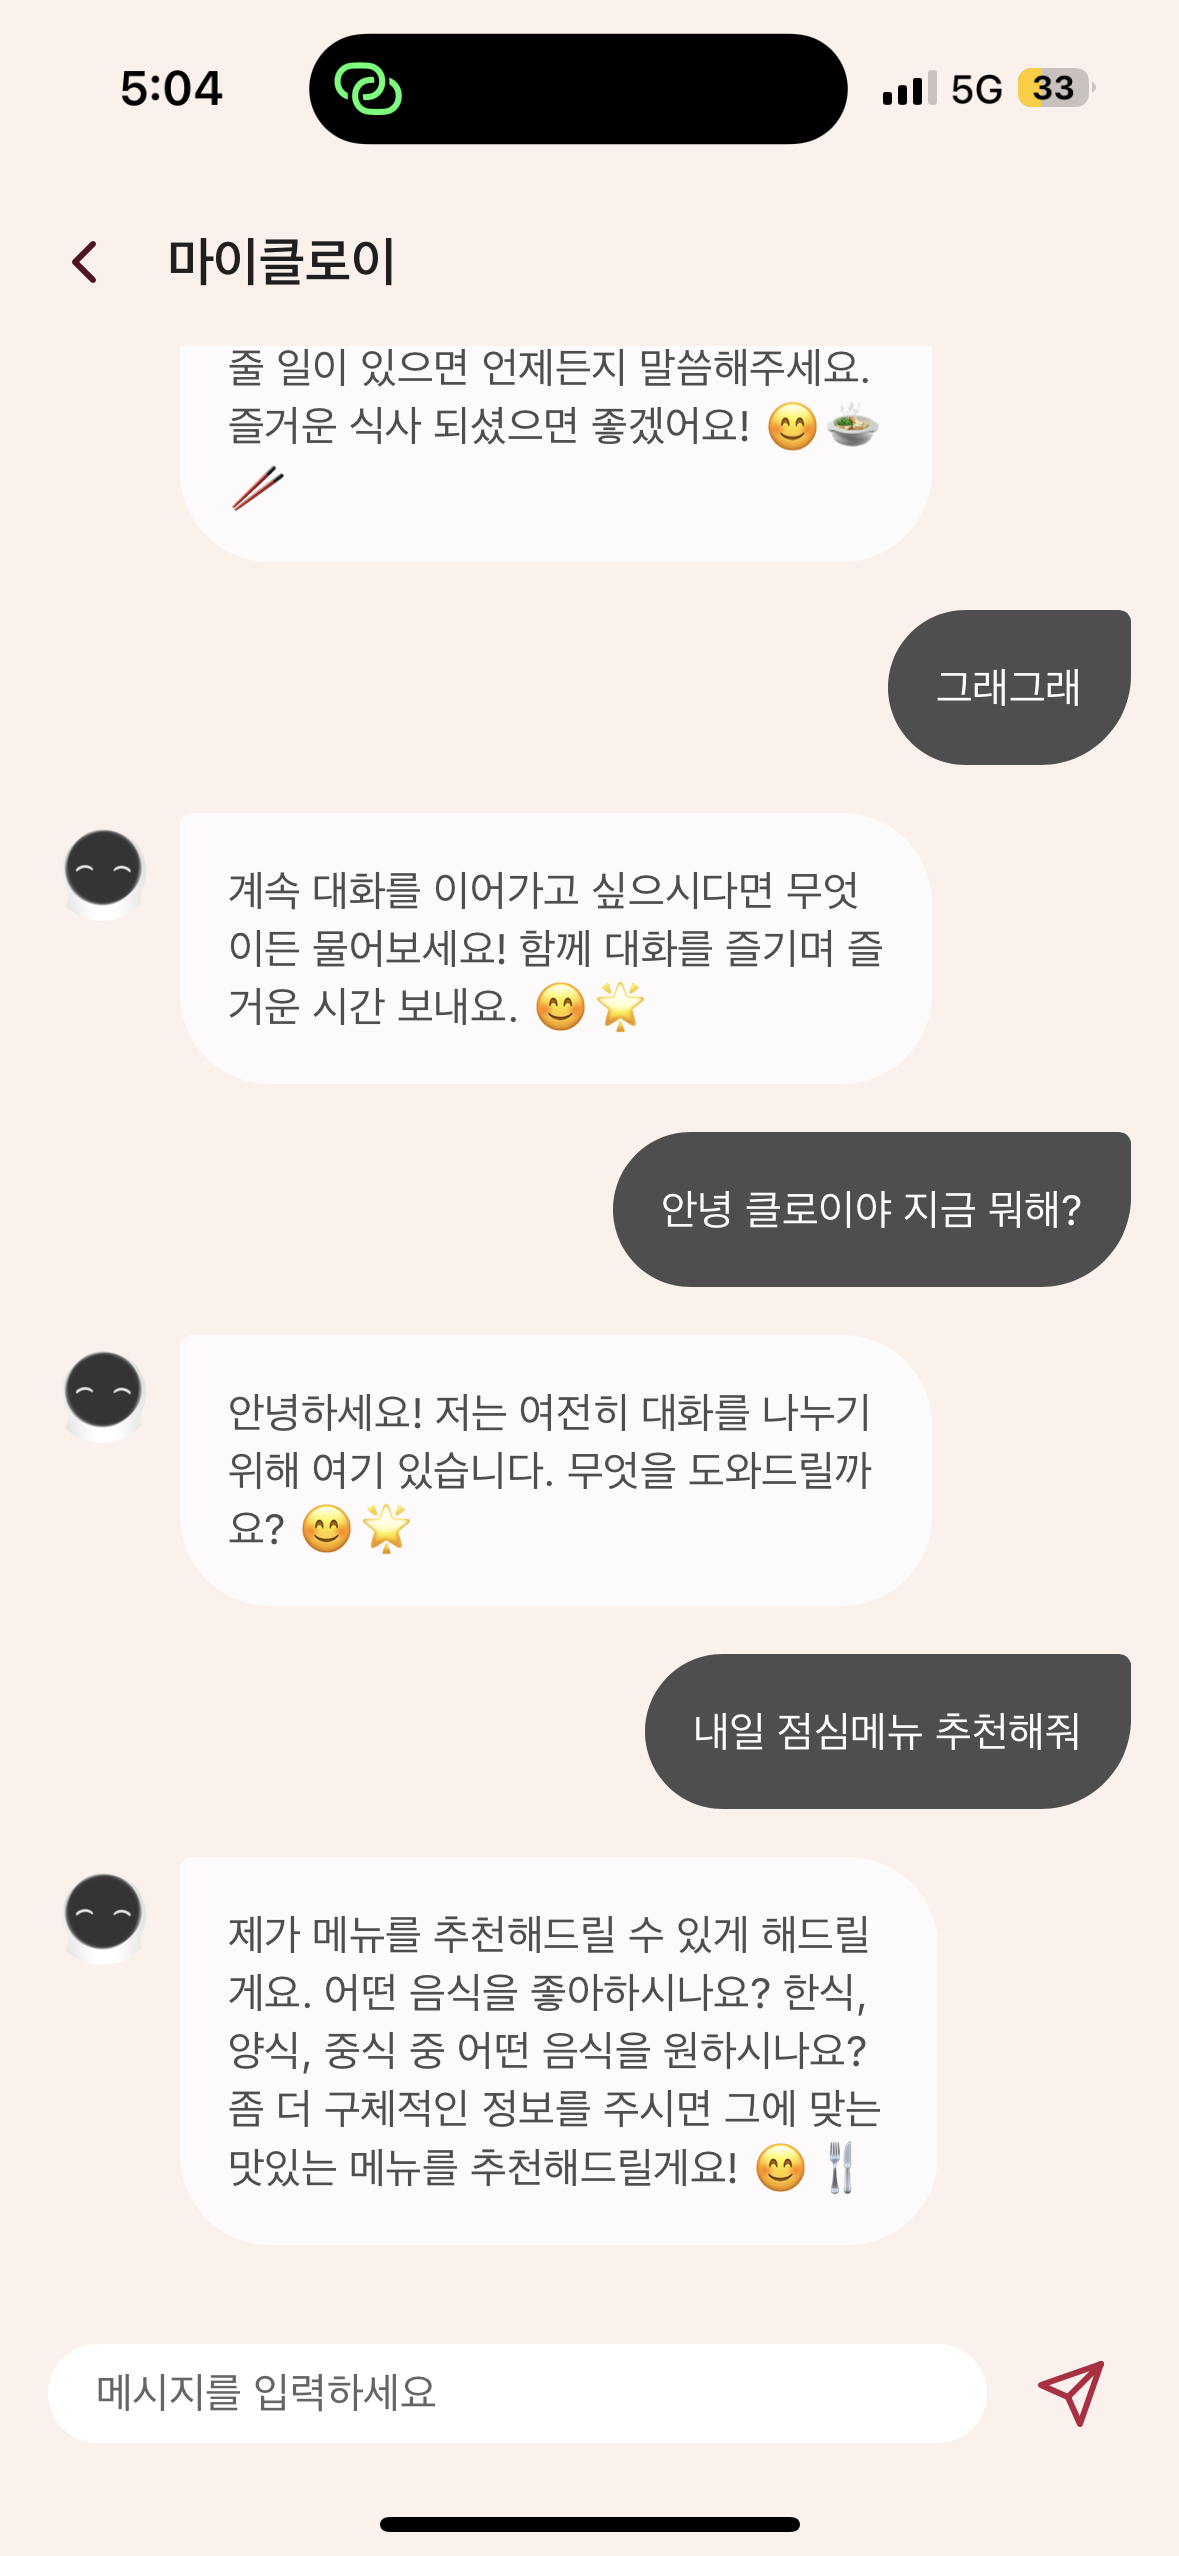
\includegraphics[width=3cm]{Images/page/chatbot.png}}
            \caption{Chatbot Page}
            \label{fig}
        \end{figure}
        The application features an AI chatbot called CLOI, which interacts with users through personalized conversations and friendly messages. CLOI serves as both a virtual companion and a dynamic feature that evolves and grows based on user engagement and activity within the platform.
        The chatbot's functionality is powered by the OpenAI API, enabling CLOI to generate contextually relevant responses based on the user's activity patterns, posting frequency, and time of day.
        The backend, built with Express.js and MongoDB, tracks user activity and manages the chatbot's evolution. The React Native frontend integrates CLOI using Zustand for state management, ensuring seamless interactions and animations for an enhanced user experience.


       \subsection{Notification Page}
        \begin{figure}[htbp]
            \centerline{
            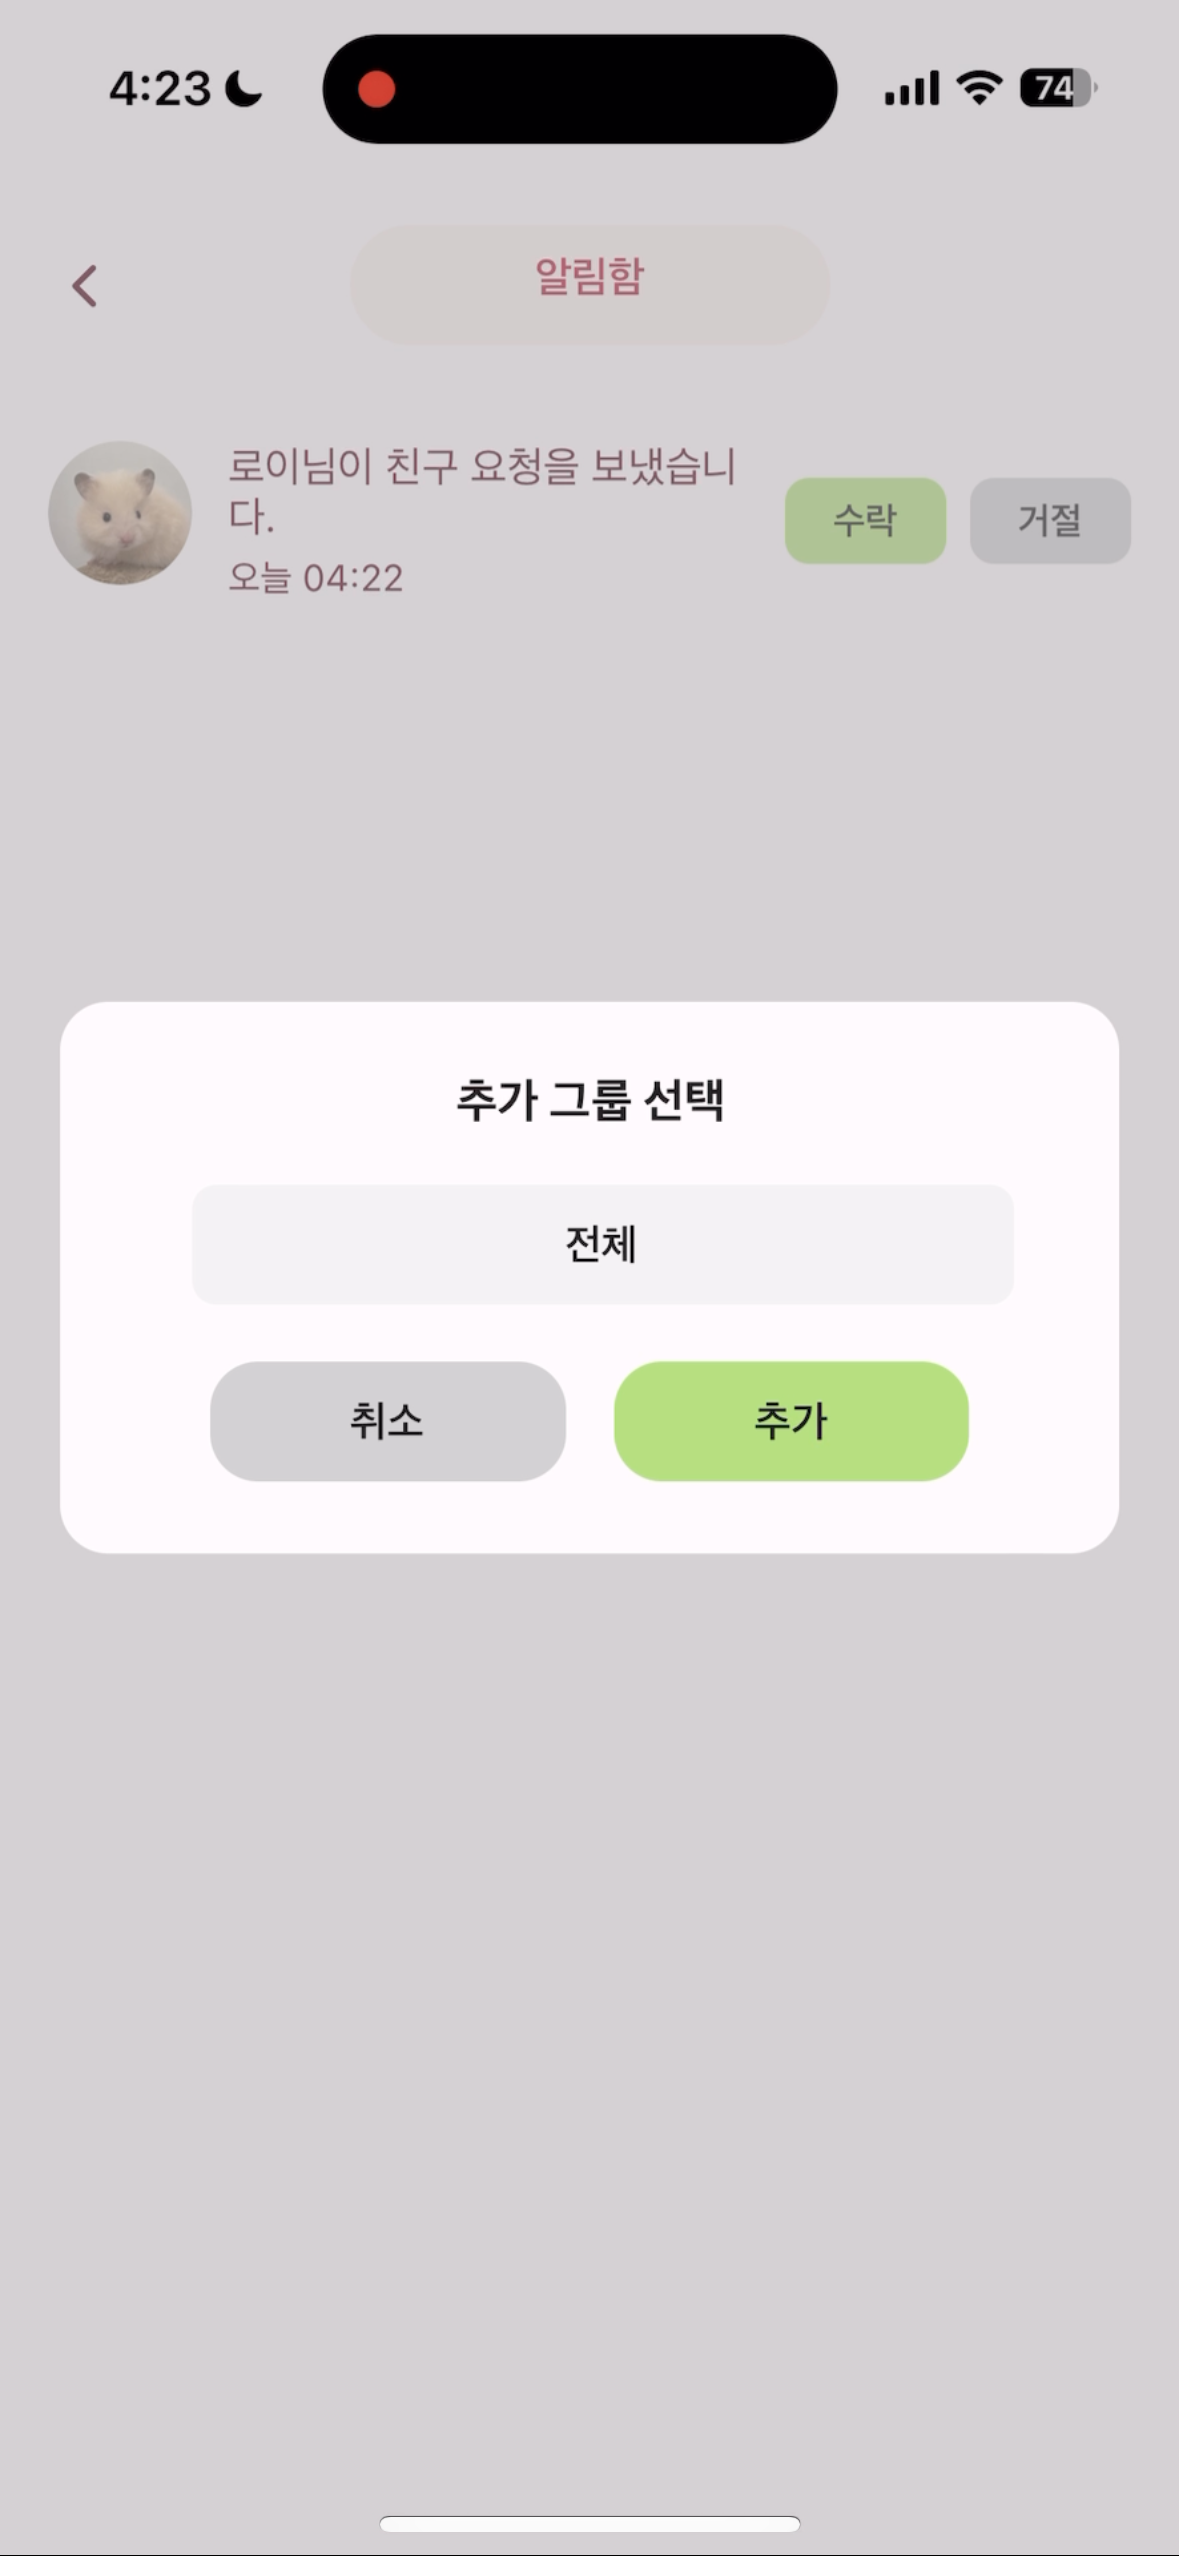
\includegraphics[width=3cm]{Images/page/notification1.png}
            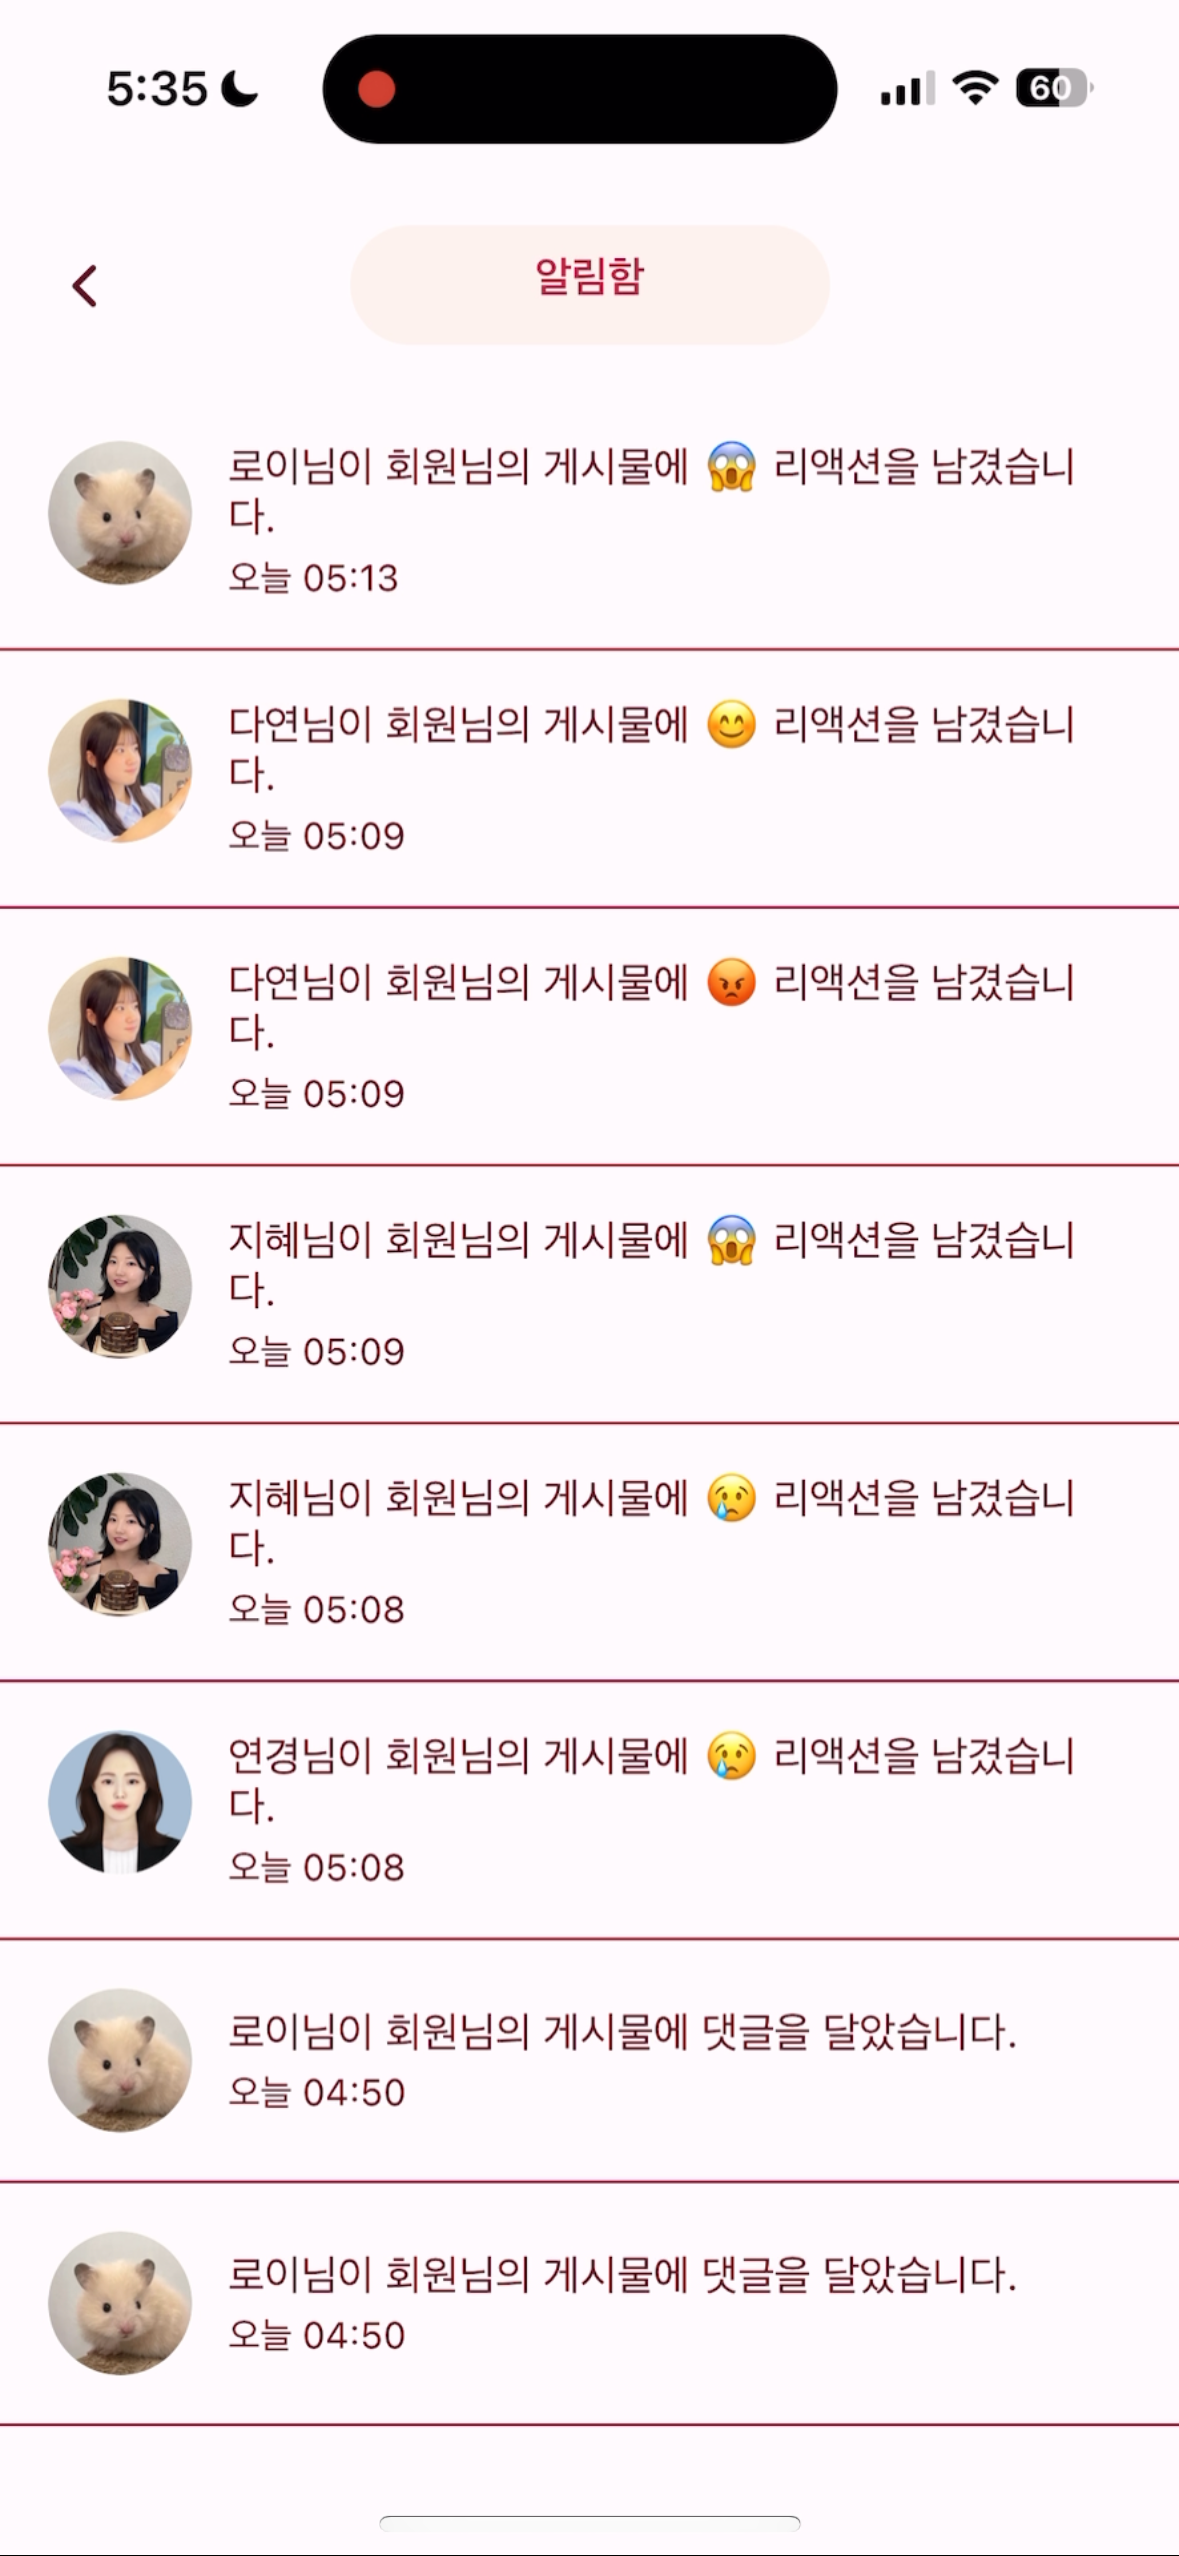
\includegraphics[width=3cm]{Images/page/notification2.png}}
              \caption{Notification Page}
            \label{fig}
        \end{figure}
        The notification system keeps users updated on activities related to their content and connections in real-time, implemented with a custom backend and MongoDB. Users can view notifications in reverse chronological order, showing details like the triggering user's profile, action performed, and timestamps. Unread notifications are visually distinct.
        Friend requests allow direct responses to accept or reject. Accepted requests let users assign friends to groups, while rejected ones remove notifications. Users can also delete individual notifications to maintain a clean interface. Notifications are generated automatically based on activities like posts, comments, or friend requests, and are stored in MongoDB with metadata for efficient management. 
        The frontend, built with React Native and Zustand, ensures seamless navigation and visual clarity. Feedback for actions, such as accepting requests, is provided through Toast notifications. An Express.js backend on Amazon EC2 handles all notification-related processes, from creation to updates and deletions, enabling a responsive, user-friendly experience that keeps users informed and engaged.

  \subsection{MyPage}
        \begin{figure}[htbp]
            \centerline{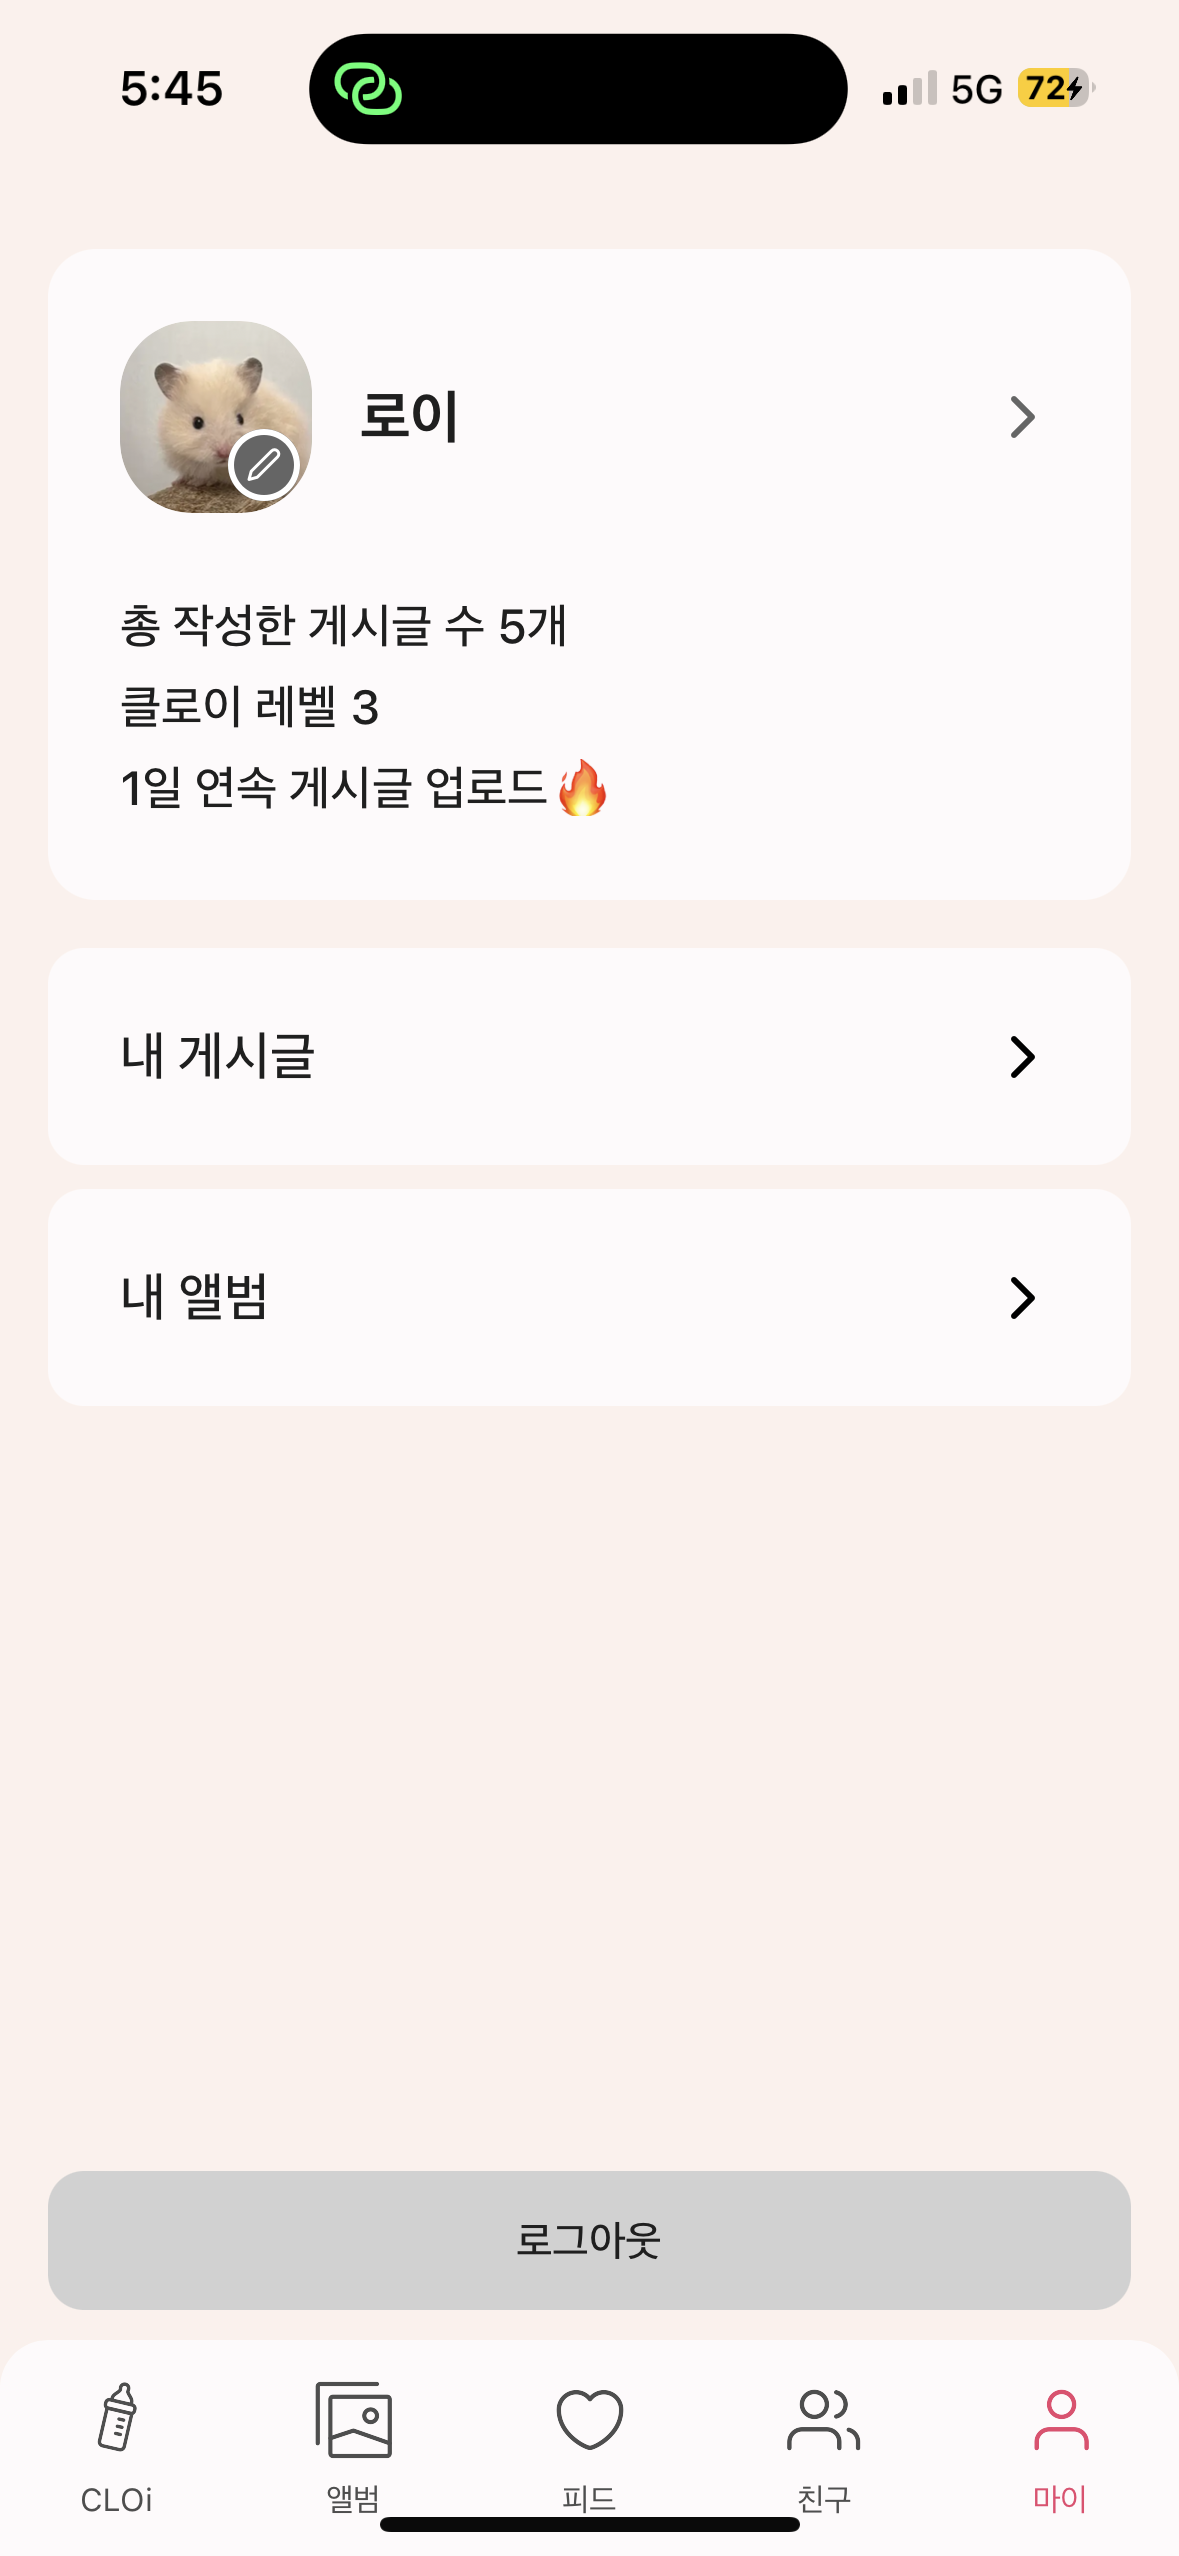
\includegraphics[width=3cm]{Images/page/mypage.png}}
            \caption{MyPage}
            \label{fig}
        \end{figure}
        The My Page serves as a personal archive space where users can manage their profile and access their content history. At the top of the page, users can view and edit their profile information, including their nickname which can be modified by tapping on it.

        The page displays key statistics about the user's activity, including the total number of posts created and their current CLOI companion level. A "10-day posting streak" badge with a fire emoji indicates active user engagement, encouraging consistent platform participation.

        The page features two main archival sections: "My Posts" and "My Album". The My Posts section provides access to a chronological feed of all text-based and AI-generated content the user has shared on the platform. The My Album section serves as a dedicated photo gallery, organizing all images the user has uploaded through their posts, whether they were AI-generated or manually uploaded from their device.

        All content data is stored in Amazon S3 with references maintained in MongoDB, while the frontend interface is built using React Native with Zustand managing the state for smooth navigation and content loading. The layout follows the application's consistent design language, providing an intuitive and organized way for users to revisit and manage their content history.

\section{Architecture Design}
    \subsection{Overall Architecture}
        Our service consists of four modules: front-end, back-end, database and AI\\
            \begin{figure}[htbp]
                \centerline{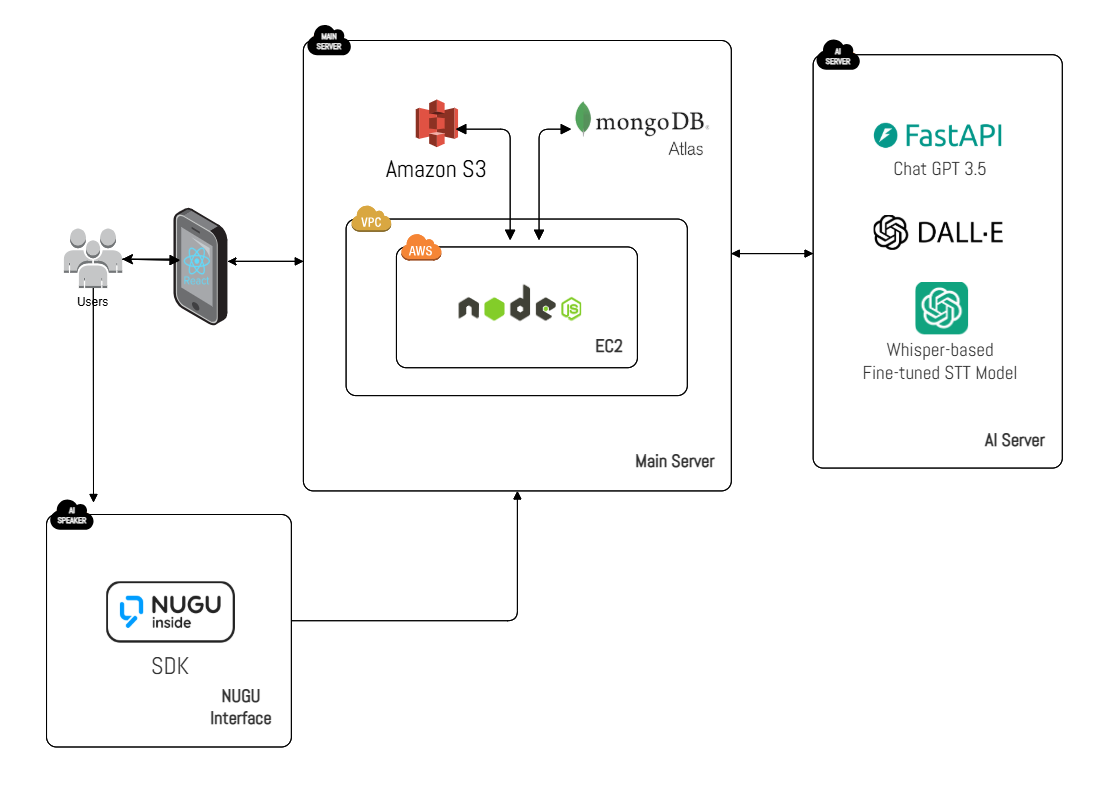
\includegraphics[width = 9.5cm, height = 6.5cm]{Images/struct/arc.png}}
                \label{fig}
                \caption{Overall Architecture}
            \end{figure}
            
                The first module is the frontend that directly interacts with the user. The frontend is developed using React Native and Expo CLI, enabling users to access backend services through the app. The app manages AI inputs (voice/text) and other SNS inputs while displaying results through HTTP communication with the backend server.
                
                The system utilizes a custom Speech-to-Text model fine-tuned on the Zeroth-Korean dataset for voice processing. The system integrates with DALL-E for image generation capabilities and ChatGPT 3.5 accessed through FastAPI for intelligent responses. The architecture supports realtime preview features through efficient client-server communication.
                
                The server-side infrastructure employs Node.js with Express on Amazon EC2, utilizing MongoDB Atlas for data storage and Amazon S3 for file management. For state management, React Hooks handle local state while Context API manages global state sharing across screens, ensuring consistent data flow throughout the application.
            
            \begin{figure}[htbp]
                \centerline{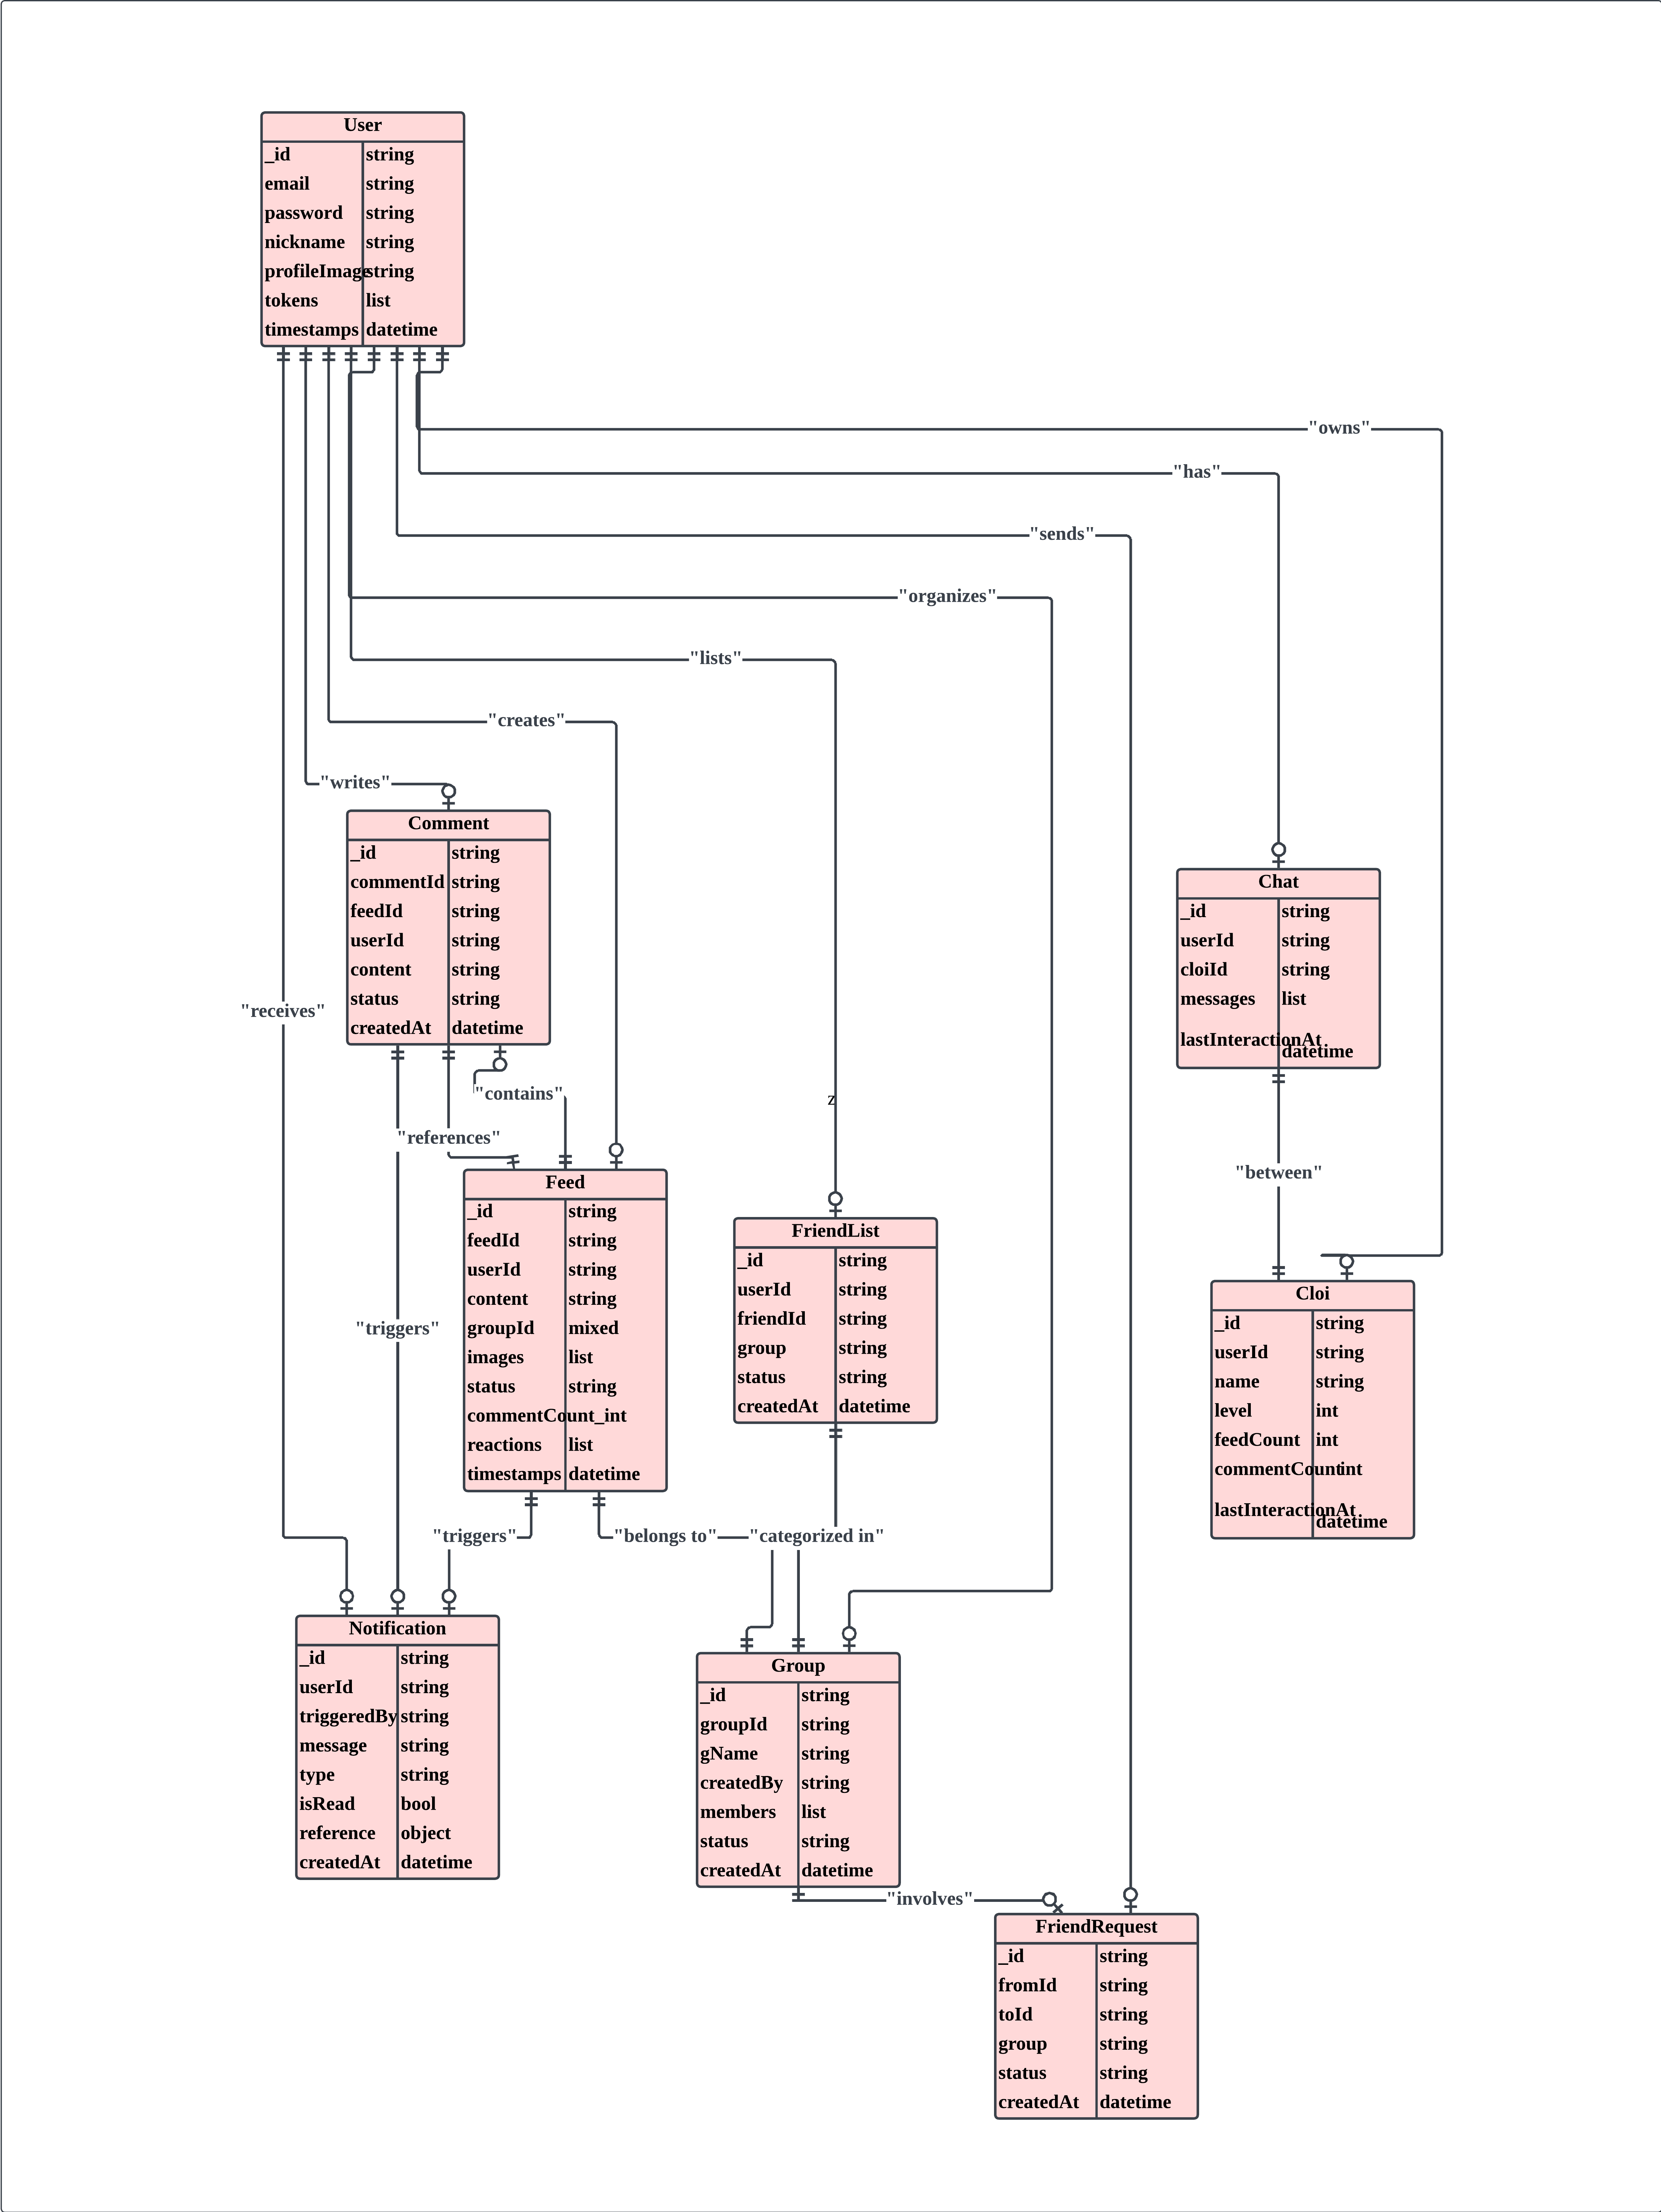
\includegraphics[width = 7cm, height = 10cm]{Images/struct/db.png}}
                \label{fig}
                \caption{Database Diagram}
            \end{figure}
            The second module is the backend system of HeartLink, which consists of a Node.js Express server, MongoDB database, and AWS S3 cloud storage. The main server manages core functionalities including user authentication, social networking features, and AI-powered interactions. All user-generated data is stored in MongoDB through the main server, which provides a robust foundation for real-time social interactions.
            
            The AI functionality is divided into three main areas and communicates with the server as follows:
            
            1. Voice Recognition: The server processes voice input using a custom STT (Speech-to-Text) model during feed creation. This model, trained on specialized datasets, converts spoken words into text in real-time. The processed text is temporarily stored in memory and directly forwarded to the FastAPI server for speech-to-text conversion. This text is then used for feed content and additional AI image generation processing.
                
            2. Image Generation: When a user requests AI image generation, the server communicates with OpenAI's DALL-E API. Text content, either manually entered or converted from voice, is sent to the DALL-E API along with specific image generation parameters. When the DALL-E API returns an image URL, the server downloads the image, converts it to a buffer, and uploads it to AWS S3 using the AWS SDK (S3Client). The server returns both the original DALL-E URL and the permanent S3 URL, which are stored in MongoDB along with the feed data.
            3. Virtual Character (Cloi): The system's AI companion Cloi interaction connects to a separate FastAPI Python server instead of directly connecting to the ChatGPT API. When users interact with Cloi, the Express server forwards requests to the FastAPI server, supporting both streaming and non-streaming responses through Server-Sent Events (SSE). The server maintains persistent connections using appropriate headers for streaming responses and includes health checks to monitor FastAPI server availability. Error handling is implemented for communication and processing failures. API responses are processed to maintain character consistency and personality according to Cloi's evolution stages (1-5).
            
            All backend components are deployed on AWS cloud infrastructure. The Node.js Express server runs on an EC2 instance (t2.micro) in the Seoul region, with proper security configurations for HTTP, HTTPS, and custom port access. The application uses PM2 for process management and Nginx as a reverse proxy, ensuring stable performance and secure communication.
            
            The system's media handling is streamlined through AWS S3 integration, using multer-s3 for efficient upload processing. Both user-uploaded and AI-generated images are stored in S3 buckets, while their references and metadata are maintained in MongoDB. This separation ensures optimal performance and scalability while maintaining data integrity.
            \vspace{3mm}
            
    \subsection{Directory Organization}
    \subsection{Module 1: Front-End}
        \subsubsection{Purpose}
            The HeartLink app provides social networking service (SNS) features that allow users to communicate and share everyday moments and memories through group feeds and group albums. Generative AI capabilities support users by enabling effortless post creation through voice recognition and text-based image generation. The front-end was developed using React Native, supporting cross-platform development and leveraging Expo to check actual app screens during development. It facilitates user-server interactions, allowing user-entered values to be stored in the backend and displaying data provided by the backend for users.\\
            \vspace{3mm}
        \subsubsection{Functionality}
            The HeartLink app's frontend enables users to log in and sign up, providing seamless access to the app while allowing easy management of user profiles and account settings. It also offers a user-friendly interface for creating posts in group feeds, utilizing AI voice recognition to input text or AI image generation to effortlessly add images. Users can view multiple group posts simultaneously through the all-group feed or visually organized content using the group album feature, which collects and displays shared images by specific groups. Through intuitive interfaces for adding friends and managing groups, users can foster communication and collaboration within groups. Additionally, the interactive UI for engaging with the virtual companion, Cloi, gamifies SNS activities, enhancing user participation and increasing the fun of the app experience.\\
            \vspace{3mm}
        \subsubsection{Location of source code}
            \begin{itemize}
                \item github.com/CSE24-HeartLink/Front-End\\
            \end{itemize}
            
            \begin{table}[]
                \centering
                \caption{Frontend Directory}
                \begin{tabular}{p{2cm}|p{2.6cm}|p{2cm}}
                    \hline
                    \textit{\textbf{Directory}} & \textit{\textbf{File Name}} & \textit{\textbf{Modules Used}}\\ 
                    \hline 
            
                    \begin{tabular}[t]{@{}l@{}}
                    Front-End/\end{tabular} & 
                    \begin{tabular}[c]{@{}l@{}}
                    .env\\.gitattributes\\.gitignore\\app.js\\app.json\\babel.config.js\\metro.config.js\\package-lock.json\\package.json\\react-native.config.js\\.prettierrc
                    \end{tabular} \\
                    \hline
            
                    \begin{tabular}[c]{@{}l@{}}
                    Front-End/assets/\\fonts/\end{tabular} & 
                    \begin{tabular}[c]{@{}l@{}}
                    pretendard fonts
                    \end{tabular} \\
                    \hline
            
                    \begin{tabular}[c]{@{}l@{}}
                    Front-End/assets/\\animations/\end{tabular} & 
                    \begin{tabular}[c]{@{}l@{}}
                    heart.json\\heartbeat.json\\Recording.json
                    \end{tabular} \\
                    \hline
                     \begin{tabular}[c]{@{}l@{}}
                    Front-End/assets/\\images/\end{tabular} & 
                    \begin{tabular}[c]{@{}l@{}}
                    AddFeed.png \\AddGroup.png \\AICollage.png \\AIdummy.png\\ChatbotButton.png \\CLOiBackground.png \\CLOiLv1.png \\CLOiLv1Face.png \\CLOiLv2.png \\CLOiLv2Face.png \\CLOiLv3.png \\CLOiLv3Face.png \\CLOiLv4.png \\CLOiLv4Face.png \\CLOiLv5.png \\CLOiLv5Face.png \\Heart.png \\Logo.png \\recording.png

                    \end{tabular} \\
                    \hline
            
                    \begin{tabular}[c]{@{}l@{}}
                    Front-End/assets/\\images/icons\end{tabular} & 
                    \begin{tabular}[c]{@{}l@{}}
                    AIImageIcon.svg\\CameraIcon.svg\\MicIcon.svg\\tabMenu1.svg\\tabMenu1active.svg\\tabMenu2.svg\\tabMenu2active.svg\\tabMenu3.svg\\tabMenu3active.svg\\tabMenu4.svg\\tabMenu4active.svg\\tabMenu5.svg\\tabMenu5active.svg
                    \end{tabular} \\
                    \hline
            
                    \begin{tabular}[c]{@{}l@{}}
                    Front-End/src/api/\end{tabular} & 
                    \begin{tabular}[c]{@{}l@{}}
                    authApi.js \\ CLOiApi.js \\ feedApi.js \\ friendApi.js \\ groupApi.js \\ notificationApi.js \\ profileApi.js \\ sttApi.js \\ websocket.js
                    \end{tabular} &
                    \begin{tabular}[c]{@{}l@{}}
                    axios \\expo-constants \\react \\react-native \\expo \\form-data \\websocket
                    \end{tabular} \\
                    \hline
            
                    \begin{tabular}[c]{@{}l@{}}
                    Front-End/src/\\components/\end{tabular} & 
                    \begin{tabular}[c]{@{}l@{}}
                    FriendItem.js\\Logo.js
                    \end{tabular} &
                    \begin{tabular}[c]{@{}l@{}}
                    react\\react-native\\@expo/vector-icons\\react-native-toast\\-message
                    \end{tabular} \\
                    \hline
              \begin{tabular}[c]{@{}l@{}}
        Front-End/src/\\components/feed/\end{tabular} & 
                \begin{tabular}[c]{@{}l@{}}
                AccountInfo.js\\CommentListModal.js\\CommentModal.js\\CommentsSection.js\\FeedItem.js\\PostContent.js\\ReactionButtons.js
                \end{tabular} &
                \begin{tabular}[c]{@{}l@{}}
                react\\react-native\\react-navigation\\/native\\@expo/vector-icons\\zustand
                \end{tabular} \\
                \hline
        
                \begin{tabular}[c]{@{}l@{}}
                Front-End/src/\\components/forms/\end{tabular} & 
                \begin{tabular}[c]{@{}l@{}}
                LoginForm.js\\SignupForm.js
                \end{tabular} &
                \begin{tabular}[c]{@{}l@{}}
                react\\react-native\\react-navigation\\/native\\zustand\\react-native-alert\\react-native-keyboard\\-aware-scroll-view
                \end{tabular} \\
                \hline
                        \end{tabular}
                    \end{table}
                    
                    \begin{table}[]
                        \centering
                        \begin{tabular}{p{2cm}|p{2.6cm}|p{2cm}}
                            \hline
                             \begin{tabular}[c]{@{}l@{}}
                Front-End/src/\\components/\\modals/\end{tabular} & 
                \begin{tabular}[c]{@{}l@{}}
                AddFriendModal.js\\AddGroupModal.js\\CLOiRenameModal.js\\DeleteConfirmModal.js\\EditGroupModal.js\\EditGroupNameModal.js\\FeedDeleteModal.js\\FriendDelete.js\\LogoutModal.js\\RenameModal.js
                \end{tabular} &
                \begin{tabular}[c]{@{}l@{}}
                react\\react-native\\react-navigation\\/native\\zustand
                \end{tabular} \\
                \hline
        
                \begin{tabular}[c]{@{}l@{}}
                Front-End/src/\\components/\\navigation/\end{tabular} & 
                \begin{tabular}[c]{@{}l@{}}
                AppNavigator.js\\BottomTabNavigator.js\\CustomBottomTabBar.js\\MainHeader.js\\RootNavigation.js
                \end{tabular} &
                \begin{tabular}[c]{@{}l@{}}
                react\\react-native\\react-navigation/stack\\react-navigation/bs\\react-native-vector-icons\\/Feather
                \end{tabular} \\
                \hline
        
                \begin{tabular}[c]{@{}l@{}}
                Front-End/src/\\components/ui/\end{tabular} & 
                \begin{tabular}[c]{@{}l@{}}
                BigCircleBackground.js\\FeedImageLoading\\Overlay.js\\FriendChoiceButton.js\\MiddleCircle\\Background.js\\MoveGroupButton.js\\PostLoadingOverlay.js\\ProfileCard.js\\ProfileImage\\LoadingOverlay.js\\ProgressBar.js\\SpeechBubble.js\\ToastConfig.js\\ToMeButton.js\\TopFilterButton.js\\TypingIndicator.js
                \end{tabular} &
                \begin{tabular}[c]{@{}l@{}}
                react\\react-native\\react-native-animatable\\react-native-vector-icons/\\Feather
                \end{tabular} \\
                \hline
                    
                    \begin{tabular}[c]{@{}l@{}}
                    Front-End/src/\\constants/\end{tabular} & 
                    \begin{tabular}[c]{@{}l@{}}
                    colors.js\\reaction.js
                    \end{tabular} \\
                    \hline
            
                    \begin{tabular}[c]{@{}l@{}}
                    Front-End/src/\\screens/\end{tabular} & 
                    \begin{tabular}[c]{@{}l@{}}
                    ChatbotScreen.js\\CLOiScreen.js\\CreatePost.js\\FeedGroupSelect\\Screen.js\\FriendsScreen.js\\GroupSelectScreen.js\\LoadingScreen.js\\LoginScreen.js\\MainFeedScreen.js\\MyPageScreen.js\\RecordScreen.js\\SignupScreen.js\\WelcomeScreen.js\\WritingGroupSelect\\Screen.js\\WritingScreen.js
                    \end{tabular} &
                    \begin{tabular}[c]{@{}l@{}}
                    react\\react-native\\react-native-vector-icons/\\Feather\\react-native-vector-icons/\\Ionicons\\react-navigation/native\\expo-image-picker
                    \end{tabular} \\
                    \hline

                    
            
                    \begin{tabular}[c]{@{}l@{}}
                    Front-End/src/\\screens/album/\end{tabular} & 
                    \begin{tabular}[c]{@{}l@{}}
                    AlbumGroupSelect\\Screen.js\\AlbumScreen.js
                    \end{tabular} &
                    \begin{tabular}[c]{@{}l@{}}
                    react\\react-native\\react-native-vector-icons/\\Feather\\@react-navigation/native
                    \end{tabular} \\
                    \hline
            
                    \begin{tabular}[c]{@{}l@{}}
                    Front-End/src/\\screens/\\notification/\end{tabular} & 
                    \begin{tabular}[c]{@{}l@{}}
                    NotificationScreen.js
                    \end{tabular} &
                    \begin{tabular}[c]{@{}l@{}}
                    react\\react-native\\react-native-vector-icons/\\Feather\\react-native-toast-message
                    \end{tabular} \\
                    \hline
            
                    \begin{tabular}[c]{@{}l@{}}
                    Front-End/src/\\screens/\\notification/\\components\end{tabular} & 
                    \begin{tabular}[c]{@{}l@{}}
                    AddFriendGroup\\Modal.js\\NotificationItem.js
                    \end{tabular} &
                    \begin{tabular}[c]{@{}l@{}}
                    react\\react-native\\react-native-vector-icons/\\Feather\\react-native-toast-message
                    \end{tabular} \\
                    \hline
            
                    \begin{tabular}[c]{@{}l@{}}
                    Front-End/src/\\store/\end{tabular} & 
                    \begin{tabular}[c]{@{}l@{}}
                    authStore.js\\chatStore.js\\CLOiStore.js\\feedStore.js\\friendStore.js\\groupStore.js\\MypageStore.js\\notificationStore.js
                    \end{tabular} &
                    \begin{tabular}[c]{@{}l@{}}
                    zustand\\@react-native-\\async-storage
                    \end{tabular} \\
                    \hline
            
                    \begin{tabular}[c]{@{}l@{}}
                    Front-End/src/utils/\end{tabular} & 
                    \begin{tabular}[c]{@{}l@{}}
                    authUtils.js\\dateUtils.js
                    \end{tabular} \\
                    \hline
                \end{tabular}
            \end{table}
            \subsubsection{Component}
                \begin{itemize}
                    \item Front-End/ : This folder contains the frontend source code of the application.
                        \item[-] .env : Environmental variables file that stores sensitive information (e.g., API keys, database URLs). Accessed through process.env in code.
                        \item[-] .gitattributes : Git configuration file that manages specific file attributes, controlling line break formats and text file processing.
                        \item[-] .gitignore : Specifies files that should not be committed to Git (e.g., node_modules, .env, log files).
                    \vspace{3mm}
                    
                    \item Front-End/assets : This folder contains various assets including fonts and images used within the app.
                        \item[-] fonts/pretendard : Font files providing basic text styles for the app.
                        \item[-] animations/ : Contains various animation json files for the app.
                        \item[-] images/ : Contains various UI elements like AddFeed.png, CLOi character images (CLOiLv1.png to CLOiLv5.png), and other interface assets.
                    \vspace{3mm}
                    
                    \item Front-End/src : This folder is the main directory containing components, API, navigation, and screens.
                    \vspace{3mm}
                    
                    \item Front-End/src/api : This folder contains API-related files for backend communication.
                        \item[-] authApi.js : Defines user authentication APIs, handling login, signup, logout, and token refresh.
                        \item[-] friendApi.js : Manages API calls for friend addition, list viewing, and deletion.
                        \item[-] groupApi.js : Defines APIs for group creation, modification, deletion, and data retrieval.
                        \item[-] notificationApi.js : Handles API requests for notification list viewing and status updates.
                        \item[-] CLOiApi.js : Handles APIs related to CLOi interactions, including information retrieval, chatting, and growth status updates.
                        \item[-] feedApi.js : Manages feed-related API calls, such as feed creation, updating, deletion, and reactions.
                        \item[-] profileApi.js : Provides APIs for user profile management, including viewing, updating, and uploading profile images.
                        \item[-] sttApi.js : Facilitates APIs for speech-to-text (STT) functionality, converting audio files into text.
                        \item[-] websocket.js : Implements WebSocket-based features, enabling real-time communication and AI-triggered events.

                    \vspace{3mm}
                    
                    \item Front-End/src/components : This folder contains custom components created for various UI elements.
                        \item[-] FriendItem.js : Component displaying each friend item in friend list, renders friend name and status, provides interaction functions.
                        \item[-] Logo.js : Component rendering app logo, used in login and welcome screens.
                    \vspace{3mm}
                    
                    \item Front-End/src/components/feed : Contains components related to feed functionality.
                        \item[-] AccountInfo.js : Displays user account information summary, including profile and account details.
                        \item[-] CommentListModal.js : Modal for showing the list of comments on a specific post.
                        \item[-] CommentModal.js : Handles comment creation or editing within a modal.
                        \item[-] CommentsSection.js : Renders the section for viewing and interacting with comments on a feed.
                        \item[-] FeedItem.js : Component that renders individual posts, including content, images, and reactions.
                        \item[-] PostContent.js : Manages the display of post content, such as text and media.
                        \item[-] ReactionButtons.js : Includes buttons for reacting to posts, such as likes or other emotions.
                    \vspace{3mm}
                
                    \item Front-End/src/components/forms : Contains components related to forms used in the app.
                        \item[-] LoginForm.js : Handles user login functionality, including form validation and submission.
                        \item[-] SignupForm.js : Provides the interface and logic for new user registration.
                    \vspace{3mm}
                
                    \item Front-End/src/components/modals : Contains modal components for various interactive functionalities.
                        \item[-] AddFriendModal.js : Modal for sending friend requests to other users.
                        \item[-] AddGroupModal.js : Modal for creating new user groups.
                        \item[-] CLOiRenameModal.js : Allows users to rename their CLOi avatar.
                        \item[-] DeleteConfirmModal.js : Prompts users for confirmation before deleting items or data.
                        \item[-] EditGroupModal.js : Modal for editing group information, such as name or members.
                        \item[-] EditGroupNameModal.js : Allows users to rename an existing group.
                        \item[-] FeedDeleteModal.js : Handles the confirmation for deleting a feed post.
                        \item[-] FriendDelete.js : Modal for removing a friend from the friend list.
                        \item[-] LogoutModal.js : Prompts users for confirmation before logging out.
                        \item[-] RenameModal.js : Generic modal for renaming items like groups or profiles.
                    \vspace{3mm}
                
                    \item Front-End/src/components/navigation : Contains navigation-related components.
                        \item[-] AppNavigator.js : Defines the app's primary navigation structure using stacks and tabs.
                        \item[-] BottomTabNavigator.js : Handles navigation between main tabs in the app.
                        \item[-] CustomBottomTabBar.js : Customizes the appearance and functionality of the bottom navigation bar.
                        \item[-] MainHeader.js : Renders the main header, including a title and navigation controls.
                        \item[-] RootNavigation.js : Manages the navigation stack and handles navigation actions globally.
                    \vspace{3mm}
                
                    \item Front-End/src/components/ui : Contains reusable UI elements for the app.
                        \item[-] BigCircleBackground.js : Provides a large circular background for decorative purposes.
                        \item[-] FeedImageLoadingOverlay.js : Displays a loading indicator while feed images are being loaded.
                        \item[-] FriendChoiceButton.js : Button component for selecting friends in group or feed contexts.
                        \item[-] MiddleCircleBackground.js : Renders a smaller circular background for design purposes.
                        \item[-] MoveGroupButton.js : Button for moving a user or item between groups.
                        \item[-] PostLoadingOverlay.js : Shows a loading overlay while posts are being uploaded.
                        \item[-] ProfileCard.js : Component for displaying user profile details, such as name and image.
                        \item[-] ProfileImageLoadingOverlay.js : Displays a loading indicator when profile images are being updated.
                        \item[-] ProgressBar.js : A visual progress indicator used for various tasks.
                        \item[-] SpeechBubble.js : A speech bubble-style UI component for comments or messages.
                        \item[-] ToastConfig.js : Configuration for displaying toast messages across the app.
                        \item[-] ToMeButton.js : A button to navigate to user-specific content or sections.
                        \item[-] TopFilterButton.js : Button for filtering content at the top of a feed or list.
                        \item[-] TypingIndicator.js : Displays a typing indicator in chat or comment sections.
                    \vspace{3mm}

                    \item Front-End/src/constants : Contains all the main constants of the application.
                    \item[-] colors.js : Contains the main color constants used throughout the application for consistent design.
                    \item[-] reactions.js : Defines emoji reactions for posts in the feed, such as smile, love, cry, and more.
                \vspace{3mm}

                    
                    \item Front-End/src/screens : Contains all the main screens of the application.
                        \item[-] ChatbotScreen.js : Screen where users interact with the chatbot for AI-driven communication.
                        \item[-] CLOiScreen.js : Screen where users can manage and interact with AI character 'CLOi', check character status/level.
                        \item[-] CreatePost.js : Screen for creating new posts.
                        \item[-] FeedGroupSelectScreen.js : Screen for selecting specific groups to view feed posts.
                        \item[-] FriendsScreen.js : Screen for managing the user's friend list, including friend requests.
                        \item[-] GroupSelectScreen.js : Screen where users can select groups to join or interact with.
                        \item[-] LoadingScreen.js : Transition screen displayed while data is being loaded.
                        \item[-] LoginScreen.js : Screen for user login, includes input fields for email and password.
                        \item[-] MainFeedScreen.js : Main screen where users can check posts in their feed, can view posts from all groups or specific groups.
                        \item[-] MyPageScreen.js : Screen for managing user profile info and personalized settings.
                        \item[-] RecordScreen.js : Screen for recording audio.
                        \item[-] SignupScreen.js : Screen for user signup, includes user info input fields and signup button.
                        \item[-] WelcomeScreen.js : Initial screen welcoming users and providing navigation options.
                        \item[-] WritingGroupSelectScreen.js : Screen for selecting a group when creating a new post or journal entry.
                        \item[-] WritingScreen.js : Screen where users can write text-based posts or entries with additional media options.
                    \vspace{3mm}
                    
                    \item Front-End/src/screens/album : Contains screens related to album functionalities.
                        \item[-] AlbumGroupSelectScreen.js : Screen for selecting groups to view shared photo albums.
                        \item[-] AlbumScreen.js : Screen displaying a specific photo album's content.
                    \vspace{3mm}
                    
                    \item Front-End/src/screens/notification : Contains screens and components for notification functionalities.
                        \item[-] NotificationScreen.js : Screen displaying a list of user notifications.
                    \vspace{3mm}
                    
                    \item Front-End/src/screens/notification/components : Contains components for notification-related interactions.
                        \item[-] AddFriendGroupModal.js : Modal for adding friends to a group through notifications.
                        \item[-] NotificationItem.js : Component for rendering individual notification items in the notification list.
                    \vspace{3mm}

                  
                    
                    \item Front-End/src/store : Contains state management files using Zustand.
                        \item[-] authStore.js : State store managing user authentication info, including login status, token management, and user data.
                        \item[-] chatStore.js : State store handling chatbot interactions, storing chat history and managing real-time messaging.
                        \item[-] CLOiStore.js : Store managing AI character 'CLOi' status, including name, level, and interactions.
                        \item[-] feedStore.js : State store managing post data, including creation, updates, reactions, and comments.
                        \item[-] friendStore.js : Store managing friend relationships, including adding, removing, and retrieving friend lists.
                        \item[-] groupStore.js : State store handling group management, including creating, updating, and deleting groups.
                        \item[-] notificationStore.js : Store managing notifications, including fetching, marking as read, and handling friend requests.
                        \item[-] profileStore.js : Store managing user profile data, including nickname, profile image, and posting statistics.
                    \vspace{3mm}

                    
                    \item Front-End/src/utils : Contains utility functions used throughout the application.
                        \item[-] authUtils.js : File containing authentication-related utility functions, defines helper functions for authentication processing.
                        \item[-] dateUtils.js : File providing utility functions for date and time formatting, including methods to format dates as '오늘', '어제', or specific dates, and to format times in `HH:MM` format.
                    \vspace{3mm}

                \end{itemize}    
        
    \subsection{Module 2: Back-End}
        \subsubsection{Purpose} 
            The backend of the HeartLink app serves as the core component that processes user requests and interacts with the database to generate appropriate responses. It receives data in JSON format from the frontend and performs Create, Read, Update, and Delete (CRUD) operations, returning the results in JSON format to the frontend and the app.
            Additionally, the backend supports essential features like group feeds, notifications, friend requests, and the growth management of the virtual character Cloi. It also handles functionalities such as file uploads, AI-based image generation, and S3 storage management.\\
            \vspace{3mm}
        \subsubsection{Functionality}
            The HeartLink app's backend processes user requests by performing CRUD operations on the database and returning the results in JSON format. It validates user authentication status using JWT token-based middleware, ensuring that only authenticated users can access specific routes. The backend manages Cloi’s state, including its level, growth, and name, and updates its development based on user activities such as posts and comments. It also enables interaction with Cloi through conversations.
            Using AWS S3 and Multer, the backend facilitates image uploads and manages the uploaded files, associating them with user feeds or group albums. It provides features for creating, modifying, and deleting user feeds, filtering feeds by friends or groups, and managing group creation, modification, deletion, and member activities. It handles friend addition, removal, and requests, as well as notifying users of friend request updates.
            Furthermore, the backend supports generating and managing notifications for user activities, such as comments, friend requests, and more. It offers features to upload, delete, and manage group album photos and provides functions to view and organize personal content, such as nicknames and profile images.\\
            \vspace{3mm}
        \subsubsection{Location of source code}
            \begin{itemize}
                \item github.com/CSE24-HeartLink/Back-End
            \end{itemize}

            \begin{table}[]
                \centering
                \caption{Backend Directory}
                \begin{tabular}{p{2.4cm}|p{2.8cm}|p{2.7cm}}
                    \hline
                    \textit{\textbf{Directory}} & \textit{\textbf{File Name}} & \textit{\textbf{Modules Used}}\\ 
                    \hline 
            
                    \begin{tabular}[c]{@{}l@{}}
                    Back-End/\end{tabular} & 
                    \begin{tabular}[c]{@{}l@{}}
                    .env\\.gitignore\\app.js\\dbclear.js\\package-lock.json\\package.json\end{tabular} &
                    \begin{tabular}[c]{@{}l@{}}
                    express\\ dotenv\\ mongoose\\ cors\\ node-cron\\ @aws-sdk/client-s3\\ uuid
                    \end{tabular} \\
                    \hline
            
                    \begin{tabular}[c]{@{}l@{}}
                    Back-End/bin/\end{tabular} & 
                    \begin{tabular}[c]{@{}l@{}}
                    www\end{tabular} &
                    \begin{tabular}[c]{@{}l@{}}
                    http\\ debug\end{tabular} \\
                    \hline
            
                    \begin{tabular}[c]{@{}l@{}}
                    Back-End/config/\end{tabular} & 
                    \begin{tabular}[c]{@{}l@{}}
                    multer.js\end{tabular} &
                    \begin{tabular}[c]{@{}l@{}}
                    multer\\ multer-s3\\@aws-sdk/client-s3\end{tabular} \\
                    \hline
            
                    \begin{tabular}[c]{@{}l@{}}
                    Back-End/constants/\end{tabular} & 
                    \begin{tabular}[c]{@{}l@{}}
                    reactions.js\end{tabular} &
                    \begin{tabular}[c]{@{}l@{}}
                    \end{tabular} \\
                    \hline
                    
                    \begin{tabular}[c]{@{}l@{}}
                    Back-End/controllers/\end{tabular} & 
                    \begin{tabular}[c]{@{}l@{}}
                    chatController.js\end{tabular} &
                    \begin{tabular}[c]{@{}l@{}}
                    mongoose\\ express\end{tabular} \\
                    \hline

                    
                    \begin{tabular}[c]{@{}l@{}}
                    Back-End/middleware/\end{tabular} & 
                    \begin{tabular}[c]{@{}l@{}}
                    auth.js\end{tabular} &
                    \begin{tabular}[c]{@{}l@{}}
                    jsonwebtoken\\ dotenv\end{tabular} \\
                    \hline
            
                    \begin{tabular}[c]{@{}l@{}}
                    Back-End/models/\end{tabular} & 
                    \begin{tabular}[c]{@{}l@{}}
                    Chat.js\\Cloi.js\\Comment.js\\Feed.js\\FriendList.js\\FriendRequest.js\\Group.js\\Notification.js\\User.js\\index.js\end{tabular} &
                    \begin{tabular}[c]{@{}l@{}}
                    mongoose\\bcryptjs\\jsonwebtoken\end{tabular} \\
                    \hline
            
                    \begin{tabular}[c]{@{}l@{}}
                    Back-End/public/\end{tabular} & 
                    \begin{tabular}[c]{@{}l@{}}
                    style.css\end{tabular} &
                    \begin{tabular}[c]{@{}l@{}}
                    Basic CSS styling\end{tabular} \\
                    \hline
            
                    \begin{tabular}[c]{@{}l@{}}
                    Back-End/routes/ai/\end{tabular} & 
                    \begin{tabular}[c]{@{}l@{}}
                    chatbotRoutes.js\\imageService.js\\imgRoutes.js\\sttRoutes.js\\index.js\end{tabular} &
                    \begin{tabular}[c]{@{}l@{}}
                    express\end{tabular} \\
                    \hline
            
                    \begin{tabular}[c]{@{}l@{}}
                    Back-End/routes/sns/\end{tabular} & 
                    \begin{tabular}[c]{@{}l@{}}
                    albumRoutes.js\\authRoutes.js\\cloiRoutes.js\\feedRoutes.js\\friendRoutes.js\\groupRoutes.js\\notifyRoutes.js\\profileRoutes.js\\index.js\end{tabular} &
                    \begin{tabular}[c]{@{}l@{}}
                    express\\mongoose\\bcryptjs\\jsonwebtoken\\multer\\multer-s3\\@aws-sdk/client-s3\\uuid\end{tabular} \\
                    \hline
                     
                    \begin{tabular}[c]{@{}l@{}}
                    Back-End/routes/nugu/\end{tabular} & 
                    \begin{tabular}[c]{@{}l@{}}
                    imageTest.js\\postUploadTest.js\\voiceCommandTest.js\\webSocketRoutes.js\\\end{tabular} &
                    \begin{tabular}[c]{@{}l@{}}
                    express\\mongoose\\ws\\axios\\dotenv\\openai\\uuid\end{tabular} \\
                    \hline
                    
                    \begin{tabular}[c]{@{}l@{}}
                    Back-End/uploads/\end{tabular} & 
                    \begin{tabular}[c]{@{}l@{}}
                    .gitkeep\end{tabular} \\
                    \hline
            
                    \begin{tabular}[c]{@{}l@{}}
                    Back-End/views/\end{tabular} & 
                    \begin{tabular}[c]{@{}l@{}}
                    error.ejs\\index.js\end{tabular} &
                    \begin{tabular}[c]{@{}l@{}}
                    EJS\end{tabular} \\
                    \hline
            
                \end{tabular}
            \end{table}
                        
            \subsubsection{Component}
                \begin{itemize}
                    \item Back-End/
                        \item[-] .env : A file that stores environment variables used by the application, including database connection details, AWS keys, and JWT secret keys, ensuring security.
                        \item[-] .gitignore : A configuration file that excludes specific files and directories from version control in Git, such as .env, node\_modules, and log files.
                        \item[-] app.js : The main server file based on Express, responsible for middleware setup, database connections, route initialization, and server startup.
                    \vspace{3mm}
                    
                    \item Back-End/bin/
                        \item[-] www : The entry point for creating an HTTP server and configuring the application to run on a specific port.
                    \vspace{3mm}
                    
                    \item Back-End/config/
                        \item[-] multer.js : A configuration file for handling file uploads using AWS S3, managing image uploads, and applying restrictions.
                    \vspace{3mm}
                    
                    \item Back-End/middleware/
                        \item[-] auth.js : Middleware for user authentication, verifying JWT tokens to ensure the user's authentication status.
                    \vspace{3mm}
                    
                    \item Back-End/models/
                        \item[-] Cloi.js : Manages data for the virtual character 'Cloi', storing growth and interaction details linked to users.
                        \item[-] Comment.js : Handles comment data associated with specific posts and users.
                        \item[-] Feed.js : Stores user post data, including group IDs, images, and status information.
                        \item[-] FriendList.js : Manages friendships between users, including group categorization and status details.
                        \item[-] FriendRequest.js : Tracks friend request data, managing request statuses such as pending, accepted, and declined.
                        \item[-] Group.js : Manages user-created group data, including member lists and statuses.
                        \item[-] Notification.js : Stores activity notification data, such as friend requests, comments, and Cloi growth updates.
                        \item[-] User.js : Manages user data, including email, encrypted passwords, nicknames, and login tokens.
                        \item[-] Chat.js : Manages chat data between users and the AI character 'Cloi', including user and assistant messages, timestamps, and last interaction time. Each chat is linked to a user and their corresponding Cloi character.

                        \item[-] index.js : Defines database schemas and includes key models.
                    \vspace{3mm}
                    
                    \item Back-End/routes/ai/
                        \item[-] chatbotRoutes.js : Handles AI chat requests by communicating with the FastAPI server, supporting both standard and streaming responses.
                        \item[-] imageService.js : Provides functionality for AI-powered image generation using OpenAI's DALL-E 3 model. Accepts a user-defined prompt and returns generated images with specified size and quality.
                        \item[-] imgRoutes.js : Generates images from text using OpenAI's DALL-E API and uploads the generated images to AWS S3.
                        \item[-] sttRoutes.js : Processes STT (Speech-to-Text) requests for voice recognition.
                        \item[-] index.js : Consolidates AI-related routes and connects sub-routes.
                    \vspace{3mm}
                    
                    \item Back-End/routes/sns/
                        \item[-] authRoutes.js : Manages user authentication requests, such as signup, login, and logout.
                        \item[-] cloiRoutes.js : Manages the state, growth, and interactions of the virtual character 'Cloi'.
                        \item[-] feedRoutes.js : Provides functionalities for creating, updating, and deleting user feeds, including image uploads.
                        \item[-] friendRoutes.js : Manages friend addition, removal, and friend requests.
                        \item[-] groupRoutes.js : Supports group creation, modification, deletion, and member management.
                        \item[-] notifyRoutes.js : Handles user notification creation and read status requests.
                        \item[-] profileRoutes.js : Processes user profile retrieval and update requests.
                        \item[-] index.js : Consolidates SNS-related routes and connects sub-routes.
                    \vspace{3mm}

                    \item Back-End/routes/nugu/
                        \item[-] imageTest.js : Tests the WebSocket functionality for generating images by sending prompts to the server and receiving generated image data.
                        \item[-] postUploadTest.js : Sends simulated voice commands for uploading posts to the server via WebSocket and verifies the responses.
                        \item[-] voiceCommandTest.js : Tests WebSocket functionality for handling voice commands, such as enabling voice recognition or triggering specific app functions.
                        \item[-] webSocketRoutes.js : Manages WebSocket server setup and handles AI-related requests, including image generation and voice commands, by broadcasting data to all connected clients.
                        \vspace{3mm}

                    
                    \item Back-End/uploads/
                        \item[-] .gitkeep : A placeholder file to maintain the upload directory in Git.
                    \vspace{3mm}
                    
                    \item Back-End/views/
                        \item[-] error.ejs : Renders error messages and stack traces when server errors occur.
                        \item[-] index.js : Renders the default welcome message displayed to clients.
                \end{itemize}
        
    \subsection{Module 3: Database}
        \subsubsection{Purpose}
            The database of the HeartLink app serves as the backbone for storing and managing all critical data related to users, feeds, comments, groups, notifications, and the virtual character Cloi. By storing this data in a structured and relational manner, the database ensures seamless functionality, efficient data retrieval, and an enhanced user experience. It supports all core functionalities of the app, including user interactions, group management, and AI-powered features.\\
            \vspace{3mm}
        \subsubsection{Functionality}
            The HeartLink database interacts with the backend server to handle all CRUD operations. When users create new data, the server leverages MongoDB Atlas to insert new entries into the database. Data retrieval is optimized through queries that utilize indexes, ensuring fast and accurate responses. User activities such as creating posts or sending friend requests trigger updates to relevant records, including notifications and Cloi's growth statistics. Additionally, when users delete content or update their profiles, the database reflects these changes in real time across the app, maintaining consistency and responsiveness.\\
            \vspace{3mm}
        \subsubsection{Component}
            \begin{itemize}
                \item User Collection\\
                The User collection stores essential information about registered users, such as their email, password, nickname, and tokens. The email field is unique and serves as the primary identifier for users, while passwords are securely encrypted using bcrypt. The tokens field tracks multiple login sessions, including device-specific data like Expo push tokens for notifications. This collection forms the foundation of the app by enabling authentication, user-specific features, and activity tracking.
                \vspace{3mm}
                \item Feed Collection\\
                The Feed collection manages posts created by users. Each feed is uniquely identified by a feedId and is associated with the user via the userId field. Additional fields include content, groupId (categorizing posts by group), and images (both user-uploaded and AI-generated). The Feed collection supports creating, updating, and deleting posts while integrating with comments and group functionalities for enhanced engagement.
                \vspace{3mm}                
                \item Comment Collection\\
                The Comment collection handles user-generated comments on posts. Each comment is uniquely identified by a commentId and is linked to a feed and a user through their respective IDs. Fields include content, creation date, and status (e.g., active or deleted). This collection facilitates user interaction and conversations within the app.
                \vspace{3mm}                
                \item Cloi Collection\\
                The Cloi collection stores data for the virtual character Cloi, linked to users via the userId field. Fields include the character's name (customizable by users), level (indicating growth), feedCount, and commentCount. Cloi's state dynamically updates based on user activities like posting feeds or commenting, enhancing the app's gamified experience.
                \vspace{3mm}                
                \item FriendList Collection\\
                The FriendList collection records friendships between users. It includes userId and friendId fields to represent the relationship between two users. An optional group field allows users to categorize their friends for better organization. The collection supports adding, removing, and managing friends within the app.
                \vspace{3mm}                
                \item FriendRequest Collection\\
                The FriendRequest collection tracks pending friend requests between users. It includes fields like fromId (requester) and toId (recipient) and a status field to denote the request's state (e.g., pending, accepted, declined). This collection integrates with the notification system to support workflows for adding friends.
                \vspace{3mm}                
                \item Group Collection\\
                The Group collection manages user-created groups with fields such as groupId, gName (group name), createdBy (group creator), and members. This collection allows users to create, edit, delete groups, and manage group-specific interactions, facilitating organized communication and sharing.
                \vspace{3mm}     
                \item Notification Collection\\
                The Notification collection stores notifications related to user activities, including friend requests, comments, and Cloi level-ups. Notifications can be marked as read and keep users informed about app events.It contains fields such as userId (recipient), triggeredBy (initiator), message, and type (e.g., friend_request, comment).
                \vspace{3mm} 
  
            \end{itemize}
    \subsection{Module 4: AI}
        \subsubsection{Purpose}
            The AI module of HeartLink integrates various AI technologies to enhance user experiences. It combines text-based conversations (ChatGPT), image generation (DALL-E), and Auto Speech Recognition (ASR) to provide rich interactive experiences. These AI services run on a FastAPI-based backend server, processing user requests in real-time. The HuggingFace Transformer's whisper model, fine-tuned for optimal Korean speech recognition, effectively converts voice input to text. Text-based conversations and image generation utilize OpenAI APIs to ensure reliable AI services.\\
            \vspace{3mm}
        \subsubsection{Functionality}
            The HeartLink app's AI module provides automatic feed generation through speech recognition and natural conversations with characters. The speech recognition model was fine-tuned from OpenAI's Whisper model using Korean speech datasets for optimal Korean language processing, enabling real-time voice-to-text conversion. The DALL-E image generation system utilizes DALL-E 3 to create high-quality 1024x1024 pixel images from text prompts, with options for URL-based access or local storage. The ChatGPT-based conversation system leverages GPT-3.5-turbo for natural language processing, supporting both streaming and standard response modes while maintaining context across messages for seamless dialogue flow.\\
            \vspace{3mm}
        \subsubsection{Location of source code}
            \begin{itemize}
                \item github.com/CSE24-HeartLink/AI\_API
            \end{itemize}

        \begin{table}[h!]
    \centering
    \caption{AI Directory}
    \begin{tabular}{p{2.4cm}|p{3cm}|p{2cm}}
        \hline
        \textit{\textbf{Directory}} & \textit{\textbf{File Name}} & \textit{\textbf{Modules Used}} \\ 
        \hline
        AI\_API/ & 
        \begin{tabular}[c]{@{}l@{}}
            Chat\_API\_1.py\\
            DALLE\_API\_1.py\\
            config.py\\
            Korean-STT.py\\
            run\_allAPI.py\\
        \end{tabular} & 
        \begin{tabular}[c]{@{}l@{}}
            fastapi\\
            openai\\
            pydantic\\
            dotenv\\
            os\\
            requests\\
            logging\\
            transformers\\
            soundfile\\
            torch\\
            huggingface\_hub\\
            datetime\\
            python-multipart\\
            uvicorn\\
            pydub\\
            ffmpeg-python\\
        \end{tabular} \\ 
        \hline
        Root Files/ & 
        \begin{tabular}[c]{@{}l@{}}
            \_\_init\_\_.py\\
            .env\\
            .gitignore\\
            asr\_api.log\\
            requirements.txt\\
            whisper\_finetuning\_for\\\_zeroth\_korean.ipynb\\
            README.md
        \end{tabular} & \\ 
        \hline
       
    \end{tabular}
\end{table}

        
        \begin{table}[h!]
            \centering
            \caption{Development Environment}
            \begin{tabular}{|p{7.4cm}|}
                \hline
                \textbf{Python Packages Used (Python 3.10)} \\ 
                \hline
                fastapi, openai, pydantic, python-dotenv, requests, transformers, soundfile, torch, huggingface\_hub, logging, datetime, os, python-multipart, uvicorn \\ 
                \hline
            \end{tabular}
        \end{table}

            
            \subsubsection{Component}
                \begin{itemize}
                    \item AI\_API/
                        \item[-] Chat\_API\_1.py : Implements real-time chat functionality using GPT-3.5-turbo with streaming and standard response modes.
                        \item[-] DALLE\_API\_1.py : Handles image generation through DALL-E 3, processing text prompts and managing generated image outputs.
                        \item[-] 
                        Korean-STT.py : Provides speech-to-text conversion using a fine-tuned Whisper model optimized for Korean language.
                        \item[-] config.py : Centralizes configuration settings for API keys, model parameters, and environment variables.
                        \item[-] run\_allAPI.py : Starts multiple AI servers (Chat, DALLE, and Korean-STT) using Uvicorn, monitors their logs, and provides graceful shutdown functionality.
                    \vspace{3mm}
                    
                    \item Root Files
                        \item[-] \_\_init\_\_.py: Initializes the package and enables Python package imports.
                        \item[-] asr\_api.log: Records API operations and error logs for automated speech recognition.
                        \item[-] .env : Secures API keys for OpenAI and HuggingFace services.
                        \item[-] .gitignore : Specifies files/directories to exclude from version control.
                        \item[-] requirements.txt : Lists all the dependencies and their versions required for the AI modules, including FastAPI, OpenAI, and Torch.
                        \item[-] whisper\_finetuning\_for\_zeroth\_korean.ipynb : Jupyter Notebook for fine-tuning the Whisper model on Korean datasets.
                        \item[-] README.md : Documents setup instructions, features, and API usage.
                        

                \end{itemize}

\newpage

\section{Use Cases}
Below is the use case table of HeartLink.\\
% \begin{table}[]
%     \centering
%     \caption{Use Case Details}
%     \renewcommand{\arraystretch}{1.5} % 행 높이 조정
%     \begin{tabular}{p{2.4cm}|p{3cm}|p{2.7cm}}
%     \hline
%     \textit{\textbf{Use Case}} & \textit{\textbf{Function Being Tested}} & \textit{\textbf{Initial System State}} \\ 
%     \hline
%     \begin{tabular}[c]{@{}l@{}}
%     System Start
%     \end{tabular} & 
%     \begin{tabular}[c]{@{}l@{}}
%     Starting the system\\ via app icon click
%     \end{tabular} & 
%     \begin{tabular}[c]{@{}l@{}}
%     System is off
%     \end{tabular} \\ 
%     \hline
%     \begin{tabular}[c]{@{}l@{}}
%     Login
%     \end{tabular} & 
%     \begin{tabular}[c]{@{}l@{}}
%     Reading login information
%     \end{tabular} & 
%     \begin{tabular}[c]{@{}l@{}}
%     System just turned on
%     \end{tabular} \\ 
%     \hline
%     \begin{tabular}[c]{@{}l@{}}
%     Login
%     \end{tabular} & 
%     \begin{tabular}[c]{@{}l@{}}
%     Rejecting incorrect login \\information
%     \end{tabular} & 
%     \begin{tabular}[c]{@{}l@{}}
%     System just turned on
%     \end{tabular} \\ 
%     \hline
%     \begin{tabular}[c]{@{}l@{}}
%     Sign-Up
%     \end{tabular} & 
%     \begin{tabular}[c]{@{}l@{}}
%     Creating a new user \\account
%     \end{tabular} & 
%     \begin{tabular}[c]{@{}l@{}}
%     System just turned on
%     \end{tabular} \\ 
%     \hline
%     \begin{tabular}[c]{@{}l@{}}
%     Main Screen
%     \end{tabular} & 
%     \begin{tabular}[c]{@{}l@{}}
%     Viewing posts from \\all user groups
%     \end{tabular} & 
%     \begin{tabular}[c]{@{}l@{}}
%     System is logged in
%     \end{tabular} \\ 
%     \hline
%     \begin{tabular}[c]{@{}l@{}}
%     Main Screen
%     \end{tabular} & 
%     \begin{tabular}[c]{@{}l@{}}
%     Navigating to group \\selection screen
%     \end{tabular} & 
%     \begin{tabular}[c]{@{}l@{}}
%     Group selection button \\visible
%     \end{tabular} \\ 
%     \hline
%     \begin{tabular}[c]{@{}l@{}}
%     Main Screen
%     \end{tabular} & 
%     \begin{tabular}[c]{@{}l@{}}
%     Navigating to specific\\ group feed
%     \end{tabular} & 
%     \begin{tabular}[c]{@{}l@{}}
%     Group list displayed
%     \end{tabular} \\ 
%     \hline
%     \end{tabular}
%     \label{tab:use_case_details}
% \end{table}

% \begin{table}[H] % 표 위치를 고정
%     \centering
%     \caption{Use Case Inputs and Outputs}
%     \renewcommand{\arraystretch}{1.2} % 행 높이 조정
%     \begin{tabular}{|p{3.5cm}|p{6.5cm}|}
%     \hline
%     \textbf{Input} & \textbf{Expected Output} \\ \hline
%     Activate app icon & System prompts user for login information \\ \hline
%     Enter email and password, click login button & Successful login; move to main screen \\ \hline
%     Enter email and password, click login button & Login failed; error message displayed \\ \hline
%     Enter name, email, and password, then click sign-up button & System confirms account creation; moves to\\login screen \\ \hline
%     Click on the all feeds tab & Displays posts from all groups the user belongs to,\\sorted chronologically \\ \hline
%     Select group selection button & Displays group feed screen for specific group \\ \hline
%     Select desired group icon & Displays group feed for the selected group \\ \hline
%     \end{tabular}
%     \label{tab:use_case_io}
% \end{table}


% \begin{longtable}{|p{3cm}|p{4cm}|p{3.5cm}|p{4cm}|p{4cm}|}
% \caption{\makebox[\textwidth]{Use Case Details}} \\ % 제목 중앙 정렬 강제
% \hline
% \textbf{Use Case} & \textbf{Function Being Tested} & \textbf{Initial System State} & \textbf{Input} & \textbf{Expected Output} \\ \hline
% \endfirsthead
% \hline
% \textbf{Use Case} & \textbf{Function Being Tested} & \textbf{Initial System State} & \textbf{Input} & \textbf{Expected Output} \\ \hline
% \endhead
% \hline
% \endfoot
% System Start & Starting the system via app icon click & System is off & Activate app icon & System prompts the user for login information \\ \hline
% Login & Reading login information & System just turned on & Enter email and password, then click login button & Successful login; move to the main screen \\ \hline
% Login & Rejecting incorrect login information & System just turned on & Enter email and password, then click login button & Login failed; error message displayed \\ \hline
% Sign-Up & Creating a new user account & System just turned on & Enter name, email, and password, then click the sign-up button & System confirms account creation; moves to the login screen \\ \hline
% Main Screen & Viewing posts from all user groups & System is logged in & Click on the all-feeds tab & Displays posts from all groups the user belongs to, sorted chronologically \\ \hline
% Main Screen & Navigating to group selection screen & Group selection button visible & Select group selection button & Displays the group feed screen for a specific group \\ \hline
% Main Screen & Navigating to a specific group feed & Group list displayed & Select the desired group icon & Displays the group feed for the selected group \\ \hline
% Group List & Creating a new group & Group list displayed & Click on the ‘+’ button & New group creation popup displayed; after entering a name, the group is added \\ \hline
% Group List & Deleting a group & Group list displayed & Select a group, then click the delete button & Group deletion confirmation popup displayed; upon confirmation, the group is deleted \\ \hline
% Group Feed & Creating a post in a specific group & Main screen displayed & Click on the add post button & Post upload options displayed \\ \hline
% Post Creation & Creating a post using voice input & Post creation in progress & Record user voice & Converts user voice into text and displays it \\ \hline
% Post Creation & Generating an image from text & Post creation in progress & Enter text, then click the generate image button & Generates an image from the provided text prompt and displays it \\ \hline
% Post Management & Editing a post & Main screen displayed & Select the post to edit, then click the edit button & Post editing screen displayed; after editing, the post is updated \\ \hline
% Post Management & Deleting a post & Main screen displayed & Select the post to delete, then click the delete button & Post deletion confirmation popup displayed; upon confirmation, the post is deleted \\ \hline
% User Archive & Viewing all user-created posts & Main screen displayed & Navigate to the ‘My’ tab and click on ‘My Posts’ & Displays all posts created by the user \\ \hline
% User Archive & Editing or deleting a post & User archive screen displayed & Select the post to edit or delete & Edit/Delete options displayed; after selection, the post is updated or deleted \\ \hline
% Group Album & Viewing posts within a specific group album & Main screen displayed & Click on the album icon & Displays shared posts in the group as thumbnail images \\ \hline
% Friend Addition & Adding a friend & Friend list displayed & Click on the ‘Add Friend’ button & Sends a friend request to the desired user \\ \hline
% Friend Management & Approving or rejecting friend requests & Friend list displayed & Click on the approve/reject button & Processes the request and updates the friend list \\ \hline
% Group Management & Changing a friend’s group & Friend list displayed & Click on the ‘Change Group’ button & Allows the user to add a friend to the desired group \\ \hline
% Virtual CLOi Growth & Growing the virtual pet CLOi through SNS activities & CLOi screen displayed & Upload posts or photos & CLOi’s level increases, with visual changes displayed \\ \hline
% Virtual CLOi Management & Renaming CLOi & CLOi screen displayed & Click on the rename button and enter a new name & CLOi’s name is updated and reflected in the UI \\ \hline
% My Page & Viewing user profile information & Main screen displayed & Click on the My Page button & Displays the user’s profile, posts, and albums \\ \hline
% My Page & Changing profile image & My Page screen displayed & Select an image and upload it & User’s profile image is updated and reflected in the UI \\ \hline
% Notifications Management & Checking new notifications & Notifications screen displayed & View notification list & New notifications are marked as read and displayed in the list \\ \hline
% \end{longtable}

\renewcommand{\arraystretch}{1.4} % 행 간격 조정
\setlength{\tabcolsep}{3pt} % 열 간격 조정
\begin{longtable}{|>{\centering\arraybackslash}p{0.15\textwidth}|>{\centering\arraybackslash}p{0.2\textwidth}|>{\centering\arraybackslash}p{0.19\textwidth}|>{\centering\arraybackslash}p{0.19\textwidth}|>{\centering\arraybackslash}p{0.2\textwidth}|}
\caption{Use Case Details} \\ % 표 제목 중앙 정렬
\hline
\textbf{Use Case} & \textbf{Function Being Tested} & \textbf{Initial System State} & \textbf{Input} & \textbf{Expected Output} \\ \hline
\endfirsthead
\hline
\textbf{Use Case} & \textbf{Function Being Tested} & \textbf{Initial System State} & \textbf{Input} & \textbf{Expected Output} \\ \hline
\endhead
\hline
\endfoot
System Start & Starting the system via app icon click & System is off & Activate app icon & System prompts the user for login information \\ \hline
Login & Reading login information & System just turned on & Enter email and password, then click login button & Successful login; move to the main screen \\ \hline
Login & Rejecting incorrect login information & System just turned on & Enter email and password, then click login button & Login failed; error message displayed \\ \hline
Sign-Up & Creating a new user account & System just turned on & Enter name, email, and password, then click the sign-up button & System confirms account creation; moves to the login screen \\ \hline
Main Screen & Viewing posts from all user groups & System is logged in & Click on the all-feeds tab & Displays posts from all groups the user belongs to, sorted chronologically \\ \hline
Main Screen & Navigating to group selection screen & Group selection button visible & Select group selection button & Displays the group feed screen for a specific group \\ \hline
Main Screen & Navigating to a specific group feed & Group list displayed & Select the desired group icon & Displays the group feed for the selected group \\ \hline
Group List & Creating a new group & Group list displayed & Click on the ‘+’ button & New group creation popup displayed; after entering a name, the group is added \\ \hline
Group List & Deleting a group & Group list displayed & Select a group, then click the delete button & Group deletion confirmation popup displayed; upon confirmation, the group is deleted \\ \hline
Group Feed & Creating a post in a specific group & Main screen displayed & Click on the add post button & Post upload options displayed \\ \hline
Post Creation & Creating a post using voice input & Post creation in progress & Record user voice & Converts user voice into text and displays it \\ \hline
Post Creation & Generating an image from text & Post creation in progress & Enter text, then click the generate image button & Generates an image from the provided text prompt and displays it \\ \hline
Post Management & Editing a post & Main screen displayed & Select the post to edit, then click the edit button & Post editing screen displayed; after editing, the post is updated \\ \hline
Post Management & Deleting a post & Main screen displayed & Select the post to delete, then click the delete button & Post deletion confirmation popup displayed; upon confirmation, the post is deleted \\ \hline
User Archive & Viewing all user-created posts & Main screen displayed & Navigate to the ‘My’ tab and click on ‘My Posts’ & Displays all posts created by the user \\ \hline
User Archive & Editing or deleting a post & User archive screen displayed & Select the post to edit or delete & Edit/Delete options displayed; after selection, the post is updated or deleted \\ \hline
Group Album & Viewing posts within a specific group album & Main screen displayed & Click on the album icon & Displays shared posts in the group as thumbnail images \\ \hline
Friend Addition & Adding a friend & Friend list displayed & Click on the ‘Add Friend’ button & Sends a friend request to the desired user \\ \hline
Friend Management & Approving or rejecting friend requests & Friend list displayed & Click on the approve/reject button & Processes the request and updates the friend list \\ \hline
Group Management & Changing a friend’s group & Friend list displayed & Click on the ‘Change Group’ button & Allows the user to add a friend to the desired group \\ \hline
Virtual CLOi Growth & Growing the virtual pet CLOi through SNS activities & CLOi screen displayed & Upload posts or photos & CLOi’s level increases, with visual changes displayed \\ \hline
Virtual CLOi Management & Renaming CLOi & CLOi screen displayed & Click on the rename button and enter a new name & CLOi’s name is updated and reflected in the UI \\ \hline
My Page & Viewing user profile information & Main screen displayed & Click on the My Page button & Displays the user’s profile, posts, and albums \\ \hline
My Page & Changing profile image & My Page screen displayed & Select an image and upload it & User’s profile image is updated and reflected in the UI \\ \hline
Notifications Management & Checking new notifications & Notifications screen displayed & View notification list & New notifications are marked as read and displayed in the list \\ \hline
\end{longtable}

\end{document}